% Copyright (C) 2014-2020 by Thomas Auzinger <thomas@auzinger.name>

\documentclass[draft,final]{vutinfth} % Remove option 'final' to obtain debug information.

% my additions
\usepackage{url}
% \usepackage[table,xcdraw]{xcolor}
\usepackage{algpseudocode}

% Load packages to allow in- and output of non-ASCII characters.
\usepackage{lmodern}        % Use an extension of the original Computer Modern font to minimize the use of bitmapped letters.
\usepackage[T1]{fontenc}    % Determines font encoding of the output. Font packages have to be included before this line.
\usepackage[utf8]{inputenc} % Determines encoding of the input. All input files have to use UTF8 encoding.

% Extended LaTeX functionality is enables by including packages with \usepackage{...}.
\usepackage{amsmath}    % Extended typesetting of mathematical expression.
\usepackage{amssymb}    % Provides a multitude of mathematical symbols.
\usepackage{mathtools}  % Further extensions of mathematical typesetting.
\usepackage{microtype}  % Small-scale typographic enhancements.
\usepackage[inline]{enumitem} % User control over the layout of lists (itemize, enumerate, description).
\usepackage{multirow}   % Allows table elements to span several rows.
\usepackage{booktabs}   % Improves the typesettings of tables.
\usepackage{subcaption} % Allows the use of subfigures and enables their referencing.
\usepackage[ruled,linesnumbered,algochapter]{algorithm2e} % Enables the writing of pseudo code.
\usepackage[usenames,dvipsnames,table]{xcolor} % Allows the definition and use of colors. This package has to be included before tikz.
\usepackage{nag}       % Issues warnings when best practices in writing LaTeX documents are violated.
\usepackage{todonotes} % Provides tooltip-like todo notes.
\usepackage{hyperref}  % Enables cross linking in the electronic document version. This package has to be included second to last.
\usepackage[acronym,toc]{glossaries} % Enables the generation of glossaries and lists fo acronyms. This package has to be included last.

% Define convenience functions to use the author name and the thesis title in the PDF document properties.
\newcommand{\authorname}{Jacob Palecek} % The author name without titles.
\newcommand{\thesistitle}{Improving Serverless Edge Computing for Network Bound Workloads} % The title of the thesis. The English version should be used, if it exists.

% Set PDF document properties
\hypersetup{
    pdfpagelayout   = TwoPageRight,           % How the document is shown in PDF viewers (optional).
    linkbordercolor = {Melon},                % The color of the borders of boxes around crosslinks (optional).
    pdfauthor       = {\authorname},          % The author's name in the document properties (optional).
    pdftitle        = {\thesistitle},         % The document's title in the document properties (optional).
    pdfsubject      = {Subject},              % The document's subject in the document properties (optional).
    pdfkeywords     = {a, list, of, keywords} % The document's keywords in the document properties (optional).
}

\setpnumwidth{2.5em}        % Avoid overfull hboxes in the table of contents (see memoir manual).
\setsecnumdepth{subsection} % Enumerate subsections.

\nonzeroparskip             % Create space between paragraphs (optional).
\setlength{\parindent}{0pt} % Remove paragraph identation (optional).

\makeindex      % Use an optional index.
\makeglossaries % Use an optional glossary.
%\glstocfalse   % Remove the glossaries from the table of contents.

% Set persons with 4 arguments:
%  {title before name}{name}{title after name}{gender}
%  where both titles are optional (i.e. can be given as empty brackets {}).
\setauthor{}{\authorname}{BSc.}{male}
\setadvisor{Univ.Prof. Dr.}{Schahram Dustdar}{}{male}

% For bachelor and master theses:
\setfirstassistant{Dr.}{Thomas Rausch}{}{male}
% \setsecondassistant{Pretitle}{Forename Surname}{Posttitle}{male}
% \setthirdassistant{Pretitle}{Forename Surname}{Posttitle}{male}

% For dissertations:
% \setfirstreviewer{Pretitle}{Forename Surname}{Posttitle}{male}
% \setsecondreviewer{Pretitle}{Forename Surname}{Posttitle}{male}

% For dissertations at the PhD School and optionally for dissertations:
% \setsecondadvisor{Pretitle}{Forename Surname}{Posttitle}{male} % Comment to remove.

% Required data.
\setregnumber{01526624}
\setdate{01}{08}{2020} % Set date with 3 arguments: {day}{month}{year}.
\settitle{\thesistitle}{Improving Serverless Edge Computing for Network Bound Workloads} % Sets English and German version of the title (both can be English or German). If your title contains commas, enclose it with additional curvy brackets (i.e., {{your title}}) or define it as a macro as done with \thesistitle.
% \setsubtitle{Optional Subtitle of the Thesis}{Optionaler Untertitel der Arbeit} 
% Sets English and German version of the subtitle (both can be English or German).

% Select the thesis type: bachelor / master / doctor / phd-school.
% Bachelor:
% \setthesis{bachelor}
%
% Master:
\setthesis{master}
\setmasterdegree{dipl.} % dipl. / rer.nat. / rer.soc.oec. / master
%
% Doctor:
%\setthesis{doctor}
%\setdoctordegree{rer.soc.oec.}% rer.nat. / techn. / rer.soc.oec.
%
% Doctor at the PhD School
%\setthesis{phd-school} % Deactivate non-English title pages (see below)

% For bachelor and master:
\setcurriculum{Software Engineering and Internet Computing}{Software Engineering und Internet Computing} % Sets the English and German name of the curriculum.

% For dissertations at the PhD School:
\setfirstreviewerdata{Affiliation, Country}
\setsecondreviewerdata{Affiliation, Country}


\begin{document}

\frontmatter % Switches to roman numbering.
% The structure of the thesis has to conform to the guidelines at
%  https://informatics.tuwien.ac.at/study-services

\addtitlepage{naustrian} % German title page (not for dissertations at the PhD School).
\addtitlepage{english} % English title page.
\addstatementpage

\begin{danksagung*}
\todo{Ihr Text hier.}
\end{danksagung*}

\begin{acknowledgements*}
\todo{Enter your text here.}
\end{acknowledgements*}

\begin{kurzfassung}
\todo{Ihr Text hier.}
\end{kurzfassung}

\begin{abstract}
\todo{Enter your text here.}
\end{abstract}

% Select the language of the thesis, e.g., english or naustrian.
\selectlanguage{english}

% Add a table of contents (toc).
\tableofcontents % Starred version, i.e., \tableofcontents*, removes the self-entry.

% Switch to arabic numbering and start the enumeration of chapters in the table of content.
\mainmatter
\newacronym{fet}{FET}{Function Execution Time}
\newacronym{csv}{CSV}{Comma separated values}
\newacronym{cpu}{CPU}{Central Processing Unit}
\newacronym{ram}{RAM}{Random Access Memory}
\newacronym{gpu}{GPU}{Grahpics Processing Unit}
\newacronym{wan}{WAN}{Wide Area Network}
\newacronym{ran}{RAN}{Radio Access Network}
\newacronym{rtt}{RTT}{Round Trip Time}
\newacronym{trt}{TRT}{Total Response Time}
\newacronym{rps}{rps}{requests per second}
\newacronym{sla}{SLA}{Service Level Agreement}
\newacronym{qos}{QoS}{Quality of Service}
\newacronym{jsq}{JSQ}{Join-the-Shortest-Queue}
\newacronym{jiq}{JIQ}{Join-the-Idle-Queue}
\newacronym{jfsq}{JFSQ}{Join-the-Fastest-of-the-Shortest-Queue}
\newacronym{jfiq}{JFIQ}{Join-the-Fastest-of-the-Idle-Queue}
\newacronym{iot}{IoT}{Internet of Things}
\newacronym{iiot}{IIoT}{Industrial Internet of Things}
\newacronym{ai}{AI}{Artificial Intelligence}
\newacronym{mec}{MEC}{Mobile Edge Computing}
\newacronym{hpa}{HPA}{Horizontal Pod Autoscaler}
\newacronym{faas}{FaaS}{Function as a Service}
\newacronym{paas}{PaaS}{Platform as a Service}
\newacronym{tdp}{TDP}{Thermal Design Power}
\newacronym{kpi}{KPI}{Key Performance Indicator}
\newacronym{iaas}{IaaS}{Infrastructure as a Service}

\chapter{Introduction}
\section{Motivation}
\section{Problem Statement}
\section{Research Questions}

\begin{enumerate}
        \item How can current scaling and placement techniques for load balancers be changed, such that the overall performance of the serverless edge computing system improves?\\\\
    Serverless (edge) computing frameworks typically already possess a mechanism for scaling and placing services. It is also typical for load balancers to be treated as "just another service", and thus identically to functions\cite{openfaas}.
    Conceptually this is not surprising since load balancers, like functions, can be scaled to handle more requests than a single instance could.
    Serverless frameworks do not, however, consider the special role load balancers play in the performance of the system in edge computing scenarios.
    To improve the performance, particularly of network bound workloads, the scaling and placement techniques used for load balancers will likely need to be changed. As a result, we need to answer the question how the used techniques in that area have to be adapted in order to realize the aspired performance improvements, while still considering the potential side effects this has on the overall system.

        \item How much of a performance improvement can be gained from optimizing the scaling, placement and decisions of load balancers in serverless edge computing systems?\\\\
    When investigating what changes could be made to increase system responsiveness in serverless edge computing, particularly for network bound workloads, load balancing stands out as an area that is likely to yield significant improvements. Current serverless computing systems do not possess the scaling, placement and load balancing mechanisms required to process requests efficiently in an edge computing scenario. Their implementation is based on the assumption of relative homogeneity in compute power and network structure one typically finds in cloud computing systems. Even serverless computing frameworks specifically built or adapted for the edge do not necessarily take the heterogeneity of edge computing environments into account when it comes to load balancing\cite{skippy}.
    This leaves the question of whether or not adapting serverless edge computing frameworks in regard to the scaling and placement of load balancers, as well as their load balancing decision mechanism, results in performance improvements, and if so, how large they likely are.
    
        \item How do edge optimized scaling and placement techniques for load balancers, including the load balancing techniques themselves, affect the overall system behavior and characteristics in regard to their key performance metrics?\\\\
    In a serverless computing framework there usually exists an interplay between a number of different components, such as the scaler and the scheduler\cite{openfaas}\cite{kubernetes}. 
    When parts of the system are now changed, in this case, the way in which load balancers behave, as well as how they are scaled and placed, this change is potentially liable to affect the rest of the system. Some of these effects would of course be intended, such as better end to end latency, but there could also be additional, potentially unwanted effects. It is thus important how exactly such changes affect the system, and what implications that has. These changes are measured in the form of key performance indicators.
\end{enumerate}
\section{Approach}
% 1 page
Our objective with this thesis is to improve serverless computing for network bound workloads. 
The improvements we aim for are focused primarily on reducing response time, which has already been identified as an issue \cite{skippy}, but are likely also translatable to efficiency gains, depending on what the implementation goals of the specific system in question are.


Our initial evaluation identified load balancing as the primary factor holding back the performance of serverless edge computing for network bound workloads, and we thus aim to make improvements in this area.
As our preliminary testing showed, the minimum requirements to make meaningful improvements in this area are that load balancers need to be distributed across the network  instead of being centralized, and that they need to make more sophisticated load balancing decisions.
To this end our goal is two-fold.
First, we want to present a method for scaling and scheduling load balancers in such a way that they are close enough to both clients and function replicas in the network to enable requests to take an efficient path between the two.
Second, we will propose a load balancing scheme that makes load balancing decisions, which take into account the network distance of clients and function replicas, as well as the replicas' performance.


To evaluate different approaches for load balancer placement and load balancing decisions we use and extend a state of the art serverless computing simulator, and ground those simulations on real data where possible by building upon existing research\cite{philipp-da}, and conducting additional experiments to inform the simulator's functioning.
This way our methodology allows us to explore scenarios beyond those feasible for live-hardware experimentation, while making sure results are as representative as possible by using performance profiles generated via experiments with actual hardware \cite{thomas-thesis}.
Apart from simulations in the context of serverless computing, we perform separate simulations and experiments in related areas, deepening the understanding and showing the relation between the challenges of serverless edge computing and the broader context.

We further explore more than just end user performance metrics, also showing how the different components present in modern serverless solutions are influenced and themselves influence methods for load balancing and placing load balancer replicas.
Through this we gain an understanding of, outline, and propose a potential solution for the engineering problems that need to be solved in order to improve serverless edge computing in practice.
\section{Structure}
Chapter 2 provides relevant background information for the technological environment this work is embedded in. In particular it outlines the concept of serverless computing, serverless edge computing, as well as describing the concepts of load balancing and service placement.
Chapter 3 explores the related work, highlighting which other works are most directly related to this one, and describing how this thesis differs from them.
Chapter 4 describes our proposed approach. After a brief overview of the general concept, it gives insight into our view of the problem domain, followed by detailed explanations of our approach and the rationale that led to it.
Chapter 5 describes the methodologies we used when evaluating our approach, explaining the serverless function as well as its relevant components, and how it informs its simulation with data from experiments on actual hardware.
Chapter 6 contains the evaluations of our approach, detailing both experiment setups and results.
These results are then discussed in chapter 7, where their implications for serverless edge, but also the limitations of our approach are explained.
Lastly, chapter 8 concludes this thesis and gives and outlook on future work.



\chapter{Background}
\section{Serverless Computing}
% got 4 pages
This section aims to give an overview of serverless computing.
Readers who are well-versed within the matter can feel free to skip this introduction, and reference it only when needed
\subsection{What serverless computing is}
Serverless computing emerged as a new computing paradigm in the context of cloud computing, which delegates infrastructure provisioning and configuration to the cloud provider to alleviate software developers from that burden.
\gls{faas} is one of the most prominent types of serverless computing products on offer.
It allows developers to specify serverless functions, which are then deployed and scaled by the cloud provider.
It is a way in which software developers architect, develop, and deploy applications that is dramatically different from more traditional approaches.
In traditional approaches, such as microservice architectures, an application is partitioned into small components which can be scaled and deployed independently of each other.
Although microservice architectures often rely on the \gls{iaas} or \gls{paas} solutions cloud providers offer, and thus abstract away the underlying infrastructure to a certain degree, developers still need to handle most scaling and application specific \gls{qos} requirements themselves.

From a developer's perspective, serverless computing is a further increase in abstraction \cite{jonasCloudProgrammingSimplified2019}.
It can be seen as the next step in an evolution away from monolithic software applications.
Where microservices and containerized deployments first partitioned a large application into several smaller applications, serverless computing continues this trend of division into smaller components, since in serverless computing applications are partitioned into individual \textit{functions}, which each perform a single action\cite{khandelwalTaureauDeconstructingServerless2020}.

\begin{figure}
    \centering
    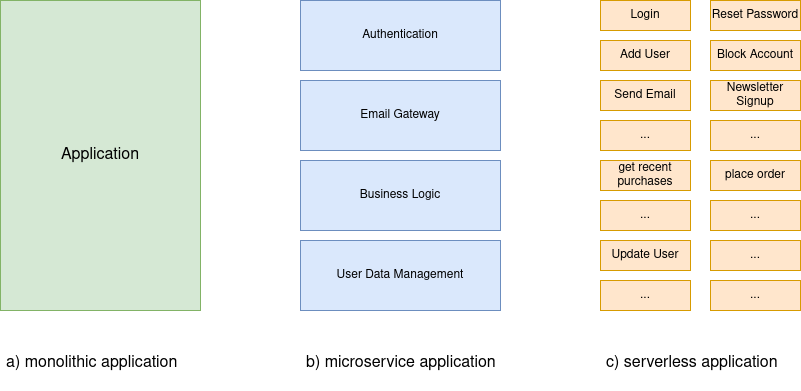
\includegraphics[width=\columnwidth]{graphics/diagrams/monolith_micro_serverless.png}
    \caption{Conceptual overview of different application architecture paradigms}
    \label{fig:mono_micro_serverless}
\end{figure}

Figure \ref{fig:mono_micro_serverless} shows this transition towards smaller partitioning of application code, leading to a higher and higher level of abstraction.
Just like microservices enabled application developers to scale different aspects of an application independently, thus enabling elasticity, serverless computing takes this even further allowing individual functions of the application to be scaled separately from each other\cite{jonasCloudProgrammingSimplified2019}.

Overall serverless affords application developers a number of advantages:
\begin{itemize}
    \item \textbf{Arbitrary elasticity:} As mentioned, serverless applications can scale their components on an extremely fine-grained level\cite{khandelwalTaureauDeconstructingServerless2020}
    \item \textbf{Abstracted infrastructure:} Where previously developers needed to be at least somewhat cognizant of the deployment of their application or its microservices, serverless enables this task to be fully delegated to the cloud provider. Developers don't necessarily need any knowledge of cloud infrastructure\cite{jonasCloudProgrammingSimplified2019}.
    \item \textbf{Precise Billing:} While in traditional cloud computing environments resources are leased for a set amount of time, irrespective of their actual usage\cite{khandelwalTaureauDeconstructingServerless2020}, serverless features a billing model where only the actual execution time and memory footprint of a function is billed down to millisecond precision\cite{jonasCloudProgrammingSimplified2019}. This allows for better resource utilization and potentially reduced costs from a customer's perspective\cite{khandelwalTaureauDeconstructingServerless2020}.
\end{itemize}

While these advantages of serverless computing over more traditional approaches are compelling, there are also idiosyncrasies of serverless computing that can, depending on the application, be problematic.
These include the need for statelessness, meaning that serverless functions have no inherent capacity to store data and would instead need to fetch it from yet another service\cite{khandelwalTaureauDeconstructingServerless2020}, or potential performance inconsistencies from cold-starts.
A cold-start, which means that the specific function code isn't running and has to be started before the request can be serviced, can occur because a serverless function wasn't executed for a certain time\cite{wangPeekingCurtainsServerless2018}.

\subsection{The architecture of serverless systems}
Architecturally, serverless systems are closely related to event based systems.
Their general concept is also very similar, since an event (i.e. a request) first arrives at the system in a form of queue, where a dispatcher or load balancer decides what action needs to be taken based on the event, and forwards it to the service (i.e. function), which ultimately processes it\cite{castroServerDeadLong2019}.

Prominent cloud based serverless platforms such as AWS Lambda\cite{aws-lambda} and Azure Functions\cite{azure-functions} are, however, proprietary and their precise architecture and inner workings are thus unknown to the public.
How these systems behave is a topic of ongoing research\cite{wangPeekingCurtainsServerless2018}, but since our research requires precise knowledge of implementation details, we choose to use open source serverless frameworks as a reference architecture of serverless systems.
These systems include Apache OpenWhisk\cite{openwhisk}, Kubeless\cite{kubeless}, and OpenFaaS\cite{openfaas}.
Since OpenFaaS has already been adapted for serverless edge computing by Rausch et al.\cite{rauschServerlessPlatformEdge}, we choose to use this open source serverless framework as the stand-in for serverless computing frameworks in general.

Architecturally, OpenFaaS is structured very similarly to the generic serverless architecture described by Castro et al.\cite{castroServerDeadLong2019}.
It too has a centralized entry-point, the Gateway, which sends requests to specific function replicas or alternatively to a queue (used for asynchronous processing and dealing with requests to functions that aren't currently running).
Each Gateway is thus effectively a load balancer for the serverless functions.
Figure \ref{fig:openfaas-gateway-diagram} shows a diagram of the architecture, as it is found in their official documentation\cite{openfaas-gateway}.

From a technical perspective, a key aspect of OpenFaaS' implementation is that it uses containers to host functions.
Containers provide an abstraction over Linux based operating systems, allowing for easier management of software dependencies, more closely controlled execution environments, and stronger application isolation.
Each function is packaged into such a container, which is an almost fully self-contained and portable artifact, that allows executing the developers' code on any machine with a compatible container runtime.
Functionally they behave similar to virtual machines, although they start up much faster, and aren't actually running individual kernels, which is why they do not provide the same level of security isolation true virtual machines do.
This choice allows functions to execute reliably, no matter the environment, and also makes it entirely agnostic to the programming language developers wish to use.
Since using containers entails their management over a cluster of multiple nodes, a task which is extremely complex, OpenFaaS\cite{openfaas} as well as other serverless frameworks build on Kubernetes\cite{kubernetes}, the de-facto industry standard container orchestration and management platform.
Building upon Kubernetes to deal with container management is a common choice among open source serverless frameworks, a choice which OpenWhisk and Kubeless make as well\cite{mohantyEvaluationOpenSource2018}.

OpenFaaS delegates a large number of tasks to the underlying Kubernetes cluster, including name resolution, request routing, which includes load balancing, and potentially scaling.
For this work, the delegation of load balancing decisions is especially important, since it implies that OpenFaaS uses whichever load balancing algorithm Kubernetes uses internally to distribute requests among function replicas.
Scaling, which determines how many instances of a serverless functions are running at any given time, can work via different mechanisms in OpenFaaS.
Depending how OpenFaaS is configured, it can either use Kubernetes' integrated \gls{hpa}\cite{kubernetes-hpa} or its own internal mechanism, which optionally allows for user customized scaling behavior\cite{openfaas-autoscaling}.
Since this work also aims to explore the impact a change in scaling and scheduling load balancers can have on the behavior of these scaling systems in general, we will now briefly describe the default scaling behavior of both \gls{hpa} and OpenFaaS' own scaler.

\subsubsection{Kubernets \gls{hpa}}
In Kubernetes scaling is typically based on either CPU or memory utilization, although in principle it can be extended with user-provided custom metrics\cite{kubernetes-hpa}.
For a given deployment, which in the context of serverless computing would be a function, a target resource value is defined.
An example would be a target average CPU utilization of 50\% for a type of function.
At that point, Kubernetes decides in a linear fashion what the desired number of replicas is.

Let $\mathbf{r_{\text{current}}}$ be the number of current replicas, $\mathbf{m_{\text{current}}}$ the current value of the metric in question and $\mathbf{m_{\text{target}}}$ the target value of the metric.
Then the target replica count is

\[ r_{\text{target}} = \left \lceil r_{\text{current}} \times \frac{m_{\text{current}}}{m_{\text{target}}} \right \rceil\]

To prevent inconsistent behavior such as replica counts oscillating Kubernetes also allows certain limiters to be set, such as minimum and maximum scales, rate of change for adding or removing replicas, and cool-downs which give the system time to stabilize before new scaling decisions are considered\cite{kubernetes-hpa}.

\subsubsection{OpenFaaS scaling}
The OpenFaaS integrated scaling mechanism is comprised of different parameters.
First a minimum and maximum scale must be set, which determine the effect of the scaling factor.
In this custom scaling variant system parameters, such as the request rate of a given function, are continuously evaluated.
Once a configured condition is met the system is notified that a given function needs to scale up or down.
The aforementioned scaling factor, which is a percentage value between 0 and 100, is then used to determine how many replicas should be started or stopped\cite{openfaas-autoscaling}.
Each scaling iteration adds or removes a number of replicas relative to the maximum scale allowed, and the scaling factor determines the size of that share.
If, for example, the maximum number of replicas is 50, and the scaling factor is 10\%, then at each scaling operation 5 replicas will be added or removed.

Which exact conditions trigger a scale up or scale down event within OpenFaaS is extremely configurable, and allows for customization based on an individual function's requirements.
By default, OpenFaaS triggers a scale-up event if the rate of rise of a function's invocation frequency exceeds a threshold over a period of time.




\section{Serverless Edge Computing}
% give a brief introduction to edge computing, just what it is + the obligatory graphic.
% what is serverless edge computing then?
% why don't current systems work well on the edge?
% give example of what it is necessary for -> edge intelligence, the bunch of applications that I've gathered, etc.
% about 2 pages should do just nicely

Serverless edge computing is an extension of existing serverless computing frameworks to the edge of the network.
It is an area of ongoing research, and aims to both further the adoption of edge computing and enable new use cases\cite{nasticServerlessRealTimeData2017}.

\subsection{Edge Computing}
Edge Computing has been proposed as a new computing paradigm to address a number of limitations and shortcomings of centralized cloud computing.
Edge Computing means that computations are not performed in a singe centralized location like a data center, but close to where the computations are needed or requested from, i.e. the edge of the network\cite{shiPromiseEdgeComputing2016}.

\begin{figure}
    \centering
    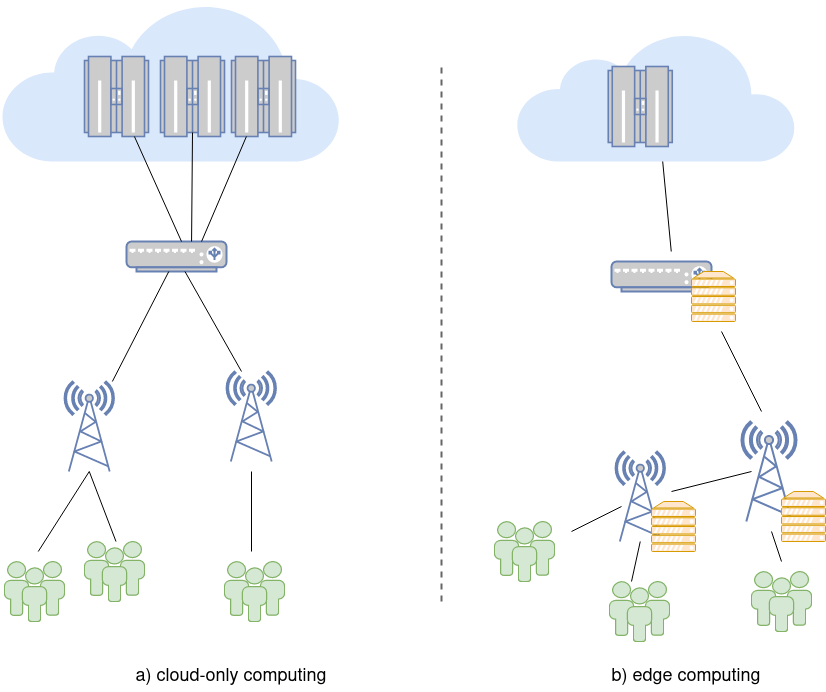
\includegraphics[width=12cm]{graphics/diagrams/edge_computing_example.png}
    \caption{An example of how in b) edge computing there are nodes interspersed throughout the network and close to clients, while in a) cloud computing all computation is centralized.}
    \label{fig:edge_comp_example}
\end{figure}

Edge computing enables a number of structural benefits that allow for the creation of new types of use-case and application.
Most notably, edge computing enables low latency, high bandwidth, computation offloading.
This can be used to improve application responsiveness, perform computations not possible on low-powered devices, or conserve energy on mobile devices by offloading complex computations to nearby edge nodes\cite{abbasMobileEdgeComputing2018b}.
Edge computing can also been seen as a way to transparently improve cloud computing, reducing the overall traffic in the network and making existing cloud applications more responsive by moving them closer to the user\cite{satyanarayananEmergenceEdgeComputing2017}.
Figure \ref{fig:edge_comp_example} shows the difference between edge and cloud computing in a simplified way.
In the example edge computing features computational nodes on \gls{ran}-towers, and thus much closer to the users.


This computing paradigm does, however, pose a challenge to existing frameworks and application architectures.
Given that computation resources are spread  farther throughout the network, the network infrastructure itself in edge computing is much more diverse\cite{shiEdgeComputingVisionChallenges2016}, potentially consisting of anything from the unreliable mobile network connection of a user's device to high bandwidth fiber networks between cloud data centers.
From both a hardware and software perspective, the computation hardware itself is more heterogeneous as well, requiring specific optimization mechanism to use resources in the most efficient way possible\cite{abbasMobileEdgeComputing2018b}.

\subsection{Serverless at the Edge}
Since serverless computing offers an abstraction layer on top of the actual infrastructure \cite{jonasCloudProgrammingSimplified2019}, and a key challenge of edge computing is that edge applications, at least up to now, have to be specifically crafted for their deployment scenario by developers\cite{shiPromiseEdgeComputing2016}.

With future \gls{ai} applications being dependent on edge computing to deliver their benefits to users via augmented reality, and smart city infrastructure\cite{rauschEdgeIntelligenceConvergence2019}, serverless offers an attractive abstraction layer to develop such \gls{ai} applications in an edge-native way.
Building on serverless as an abstraction layer for the application, the idea is that it will be able to jointly provide the benefits afforded by edge computing and serverless computing at the same time.
Functions are supposed to be deployed to nodes close to the users that rely on these functions, be scaled automatically, and routed efficiently, without any manual intervention from developers.

Achieving such a computing infrastructure would enable a host of new types of application, such as wearable cognitive assistance\cite{haWearableCognitiveAssistance2014}\cite{rauschPlatformSmartCityScale2021}, offloading \gls{ai} inference tasks from devices with low compute capability\cite{liEdgeAIOnDemand2020}, and analyzing video feeds in real time to improve public safety\cite{zhangEdgeVideoAnalytics2019}, for example to ensure face masks are worn where mandated\cite{wangWearMaskFastInbrowser2021}.

Open source serverless frameworks have been evaluated in terms of their performance in edge-scenarios, but in their current, unmodified state they lack the full set of capabilities needed to provide all the benefits edge computing offers\cite{paladeEvaluationOpenSource2019}.
While some of these serverless frameworks have been adapted to address the challenges posed by the edge computing environment, or to be better tailored to workloads related to \gls{ai}\cite{rauschServerlessPlatformEdge}, more of which will be discussed in the next chapter, overall there remain a lot of challenges for the universal practical application of serverless edge computing\cite{aslanpourServerlessEdgeComputing2021}.
Optimizing the performance of network bound workloads, for example, is one such challenge\cite{skippy}, and the one this thesis aims to address.




\section{Load Balancing}
\section{Service Placement}
% Target: 5ish pages of text
\chapter{Related Work}
% target: 8-10ish pages
\chapter{Overview}
The goal of this chapter is to give an overview of the general evaluation setup and methodology behind our approach, as this ties together the relation between our approach and its evaluation.
First, the approach we present is the result of several iterations of design and experimentation, as one would expect in the field of distributed systems engineering.
While the evaluation, of course, focuses on evaluating the solution we propose, we also include some of the experiments that led to the design and parametrization of our approach.
We decided to include these, as they highlight the broader problem area our approach addresses, and we believe them to be helpful for a deeper understanding of how our approach works.

Second, we mostly rely on simulated environments for the development and evaluation of our approach, because actual deployments in systems of the size this work addresses are infeasible, at least in the context of this work.
Thus we also use this chapter to explain the simulation environment in detail to make results more transparent, and give subsequent research the chance to potentially build not only on the results of this work, but on the environment it is built upon.
% 
\section{Simulating Serverless Edge Computing Systems}
\section{Network Topologies and Simulations}
% 1 page
\section{Using Empirical Data in Simulations}
As already described that FaaS-Sim\cite{faas-sim-github}, the serverless simulator we use, is a trace-driven simulator\cite{thomas-thesis}, meaning that it relies on measurements of real world data to make its results more representative.
The types of empirical data that can be used to improve simulation accuracy are very broad, but are typically limited to those that actually affect the metrics one is interested in measuring.
Usually this includes the memory consumption, CPU utilization, network utilization and storage size of different software components present in the system.
It can, however, also include more specific metrics such as deployment, staring, stopping and teardown times of container in a Kubernetes cluster\cite{skippy}.

Similar to how Raith et al. extended FaaS-Sim to include traces of real function executions to better represent \glspl{fet} \cite{philipp-da}, we perform experiments to inform how load balancers are modelled within the system.
Since in current serverless frameworks ingress-points, which is equivalent to a load balancer in our case, are considered as just another service, they compete with function replicas for resources.
As a result the resource usage of typical application level load balancers is an important metric for us to capture and integrate into the serverless simulator.

For our empirical evaluations we use a real Kubernetes cluster that features a variety of heterogeneous nodes.
Since we deal with edge computing applications, and resource heterogeneity is a core challenge of edge computing\cite{shiEdgeComputingVisionChallenges2016}, having a range of different nodes to evaluate performance on is critical to account for variance incurred by the use of different types of devices.
We also make use of and extend galileo\cite{galileo-github}\cite{operating-energy-aware-galileo}, a framework built for distributed load testing, as it allows us to easily define request patterns and loads that then get executed.
By using this we can go beyond measurements of baseline resource consumption and examine the relationship between the request load of a service and its performance and resource consumption profile.
To gather performance data of individual containers in a Kubernetes cluster, galileo relies on and integrates with telemd\cite{telemd-github}.
Telemd is a daemon application that can gather a number of system metrics at specifid intervals, including CPU utilization, memory consumption, disk I/O, and network transfers.


% what do I actually want to say?
% empirical experiments important to inform real world data
% need to be aligned with the hardware simulated e.g. arm devices, x86, etc. etc.
% this needs to be measured somehow -> galileo
%
%
% 1-2 pages
\section{Captured Metrics}
% Target: 20ish pages total; 13 pages of text, 7 pages of images
\chapter{Load Balancers and Their Placement}
In this chapter we describe our chosen approach for improving the performance of network bound workloads in serverless edge computing environments. We start by explaining our considerations when developing our approach in the context of a serverless edge computing system, and showing in what way our solution changes the system. From there we go into detail about how the load balancing mechanism of our solution works, how it is different from the currently employed methods, and how the choices made in regard to the load balancing method inform other parts of the proposed approach.
Lastly we go into our approach to scaling and scheduling load balancers among the nodes present in the serverless edge computing system. We make use of osmotic scaling and scheduling, a method previously outlined in existing literature. Using this idea of osmotic scaling and scheduling, we provide a concrete implementation of such an approach for placing and deciding on the number of load balancers in the system. The implementation is designed with current state of the art systems such as Kubernetes as the basis, and can thus be used as a reference implementation for use outside of a simulation context. The approach also addresses the challenges of edge computing environments that make current approaches, developed with the cloud in mind, unsuitable. Specifically our approach addresses issues of location awareness, device and network heterogeneity, and dynamically changing workload conditions.
% Target: 2ish pages \w graphics
\section{Concept}
% Note: mention that in our context load balancing and entry-gateway are sort of equivalent. Show their relation a bit
% Note: Mention that our approach uses the method of using real-life experiments to inform simulation

To understand the approach we first take a step back to view the boarder technical context the solution addresses and is built around.
As previously outlined, our solution aims to improve the performance of network bound workloads.
In the context of serverless edge computing systems network bound workloads are characterized by the network being the main or a significant contributing factor to the overall response time.
\begin{figure}
    \centering
    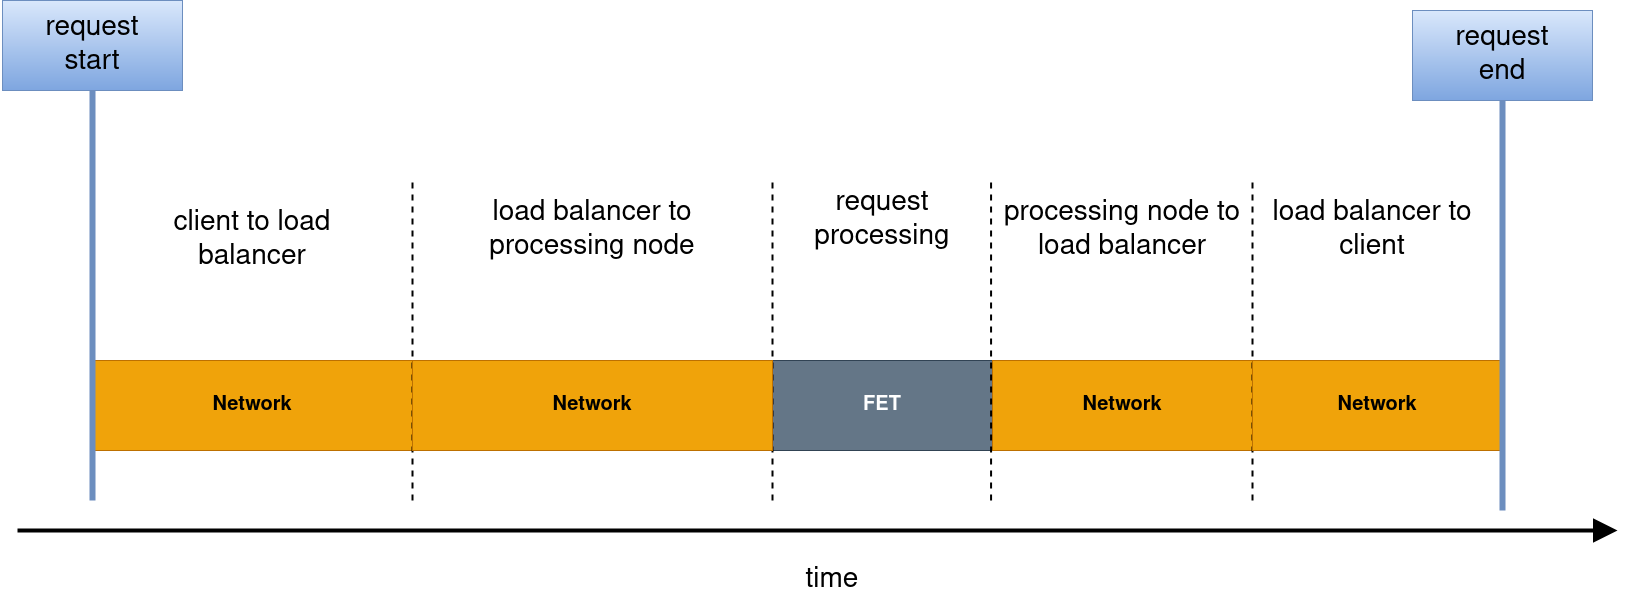
\includegraphics[width=14cm]{graphics/diagrams/request_overview.png}
    \caption{A generic view of the different parts that make up the total request processing time from the perspective of our approach}
    \label{fig:request_net_fet_overview}
\end{figure}
In Figure \ref{fig:request_net_fet_overview} we can see the different processing steps we consider for a request.
A network bound workload in this sense is one where the time taken up by the network portion of handling the request is proportionally speaking significantly larger than the portion taken by the \gls{fet}.
This is typically the case because either the request contains a lot of data that needs to be transported, or because the \gls{fet} is very short.

The primary way by which our approach improves the response times of network bound workloads is thus by reducing the amount of time spent on the network transfer portion of handling a client request.
While optimizing \glspl{fet} is not the primary objective of our approach, at least from a systems design perspective, it still has the potential to additionally reduce \glspl{fet} compared to current methods.
We consider the structure and makeup of the serverless computing system to be a given factor. As a result our approach aims to reduce network times not by changing the network makeup itself, but by utilizing the existing resources as effectively as possible. From a network-optimization perspective this means that each request should take an optimal path from  the client to the node where the request is ultimately processed. 

\begin{figure}
    \centering
    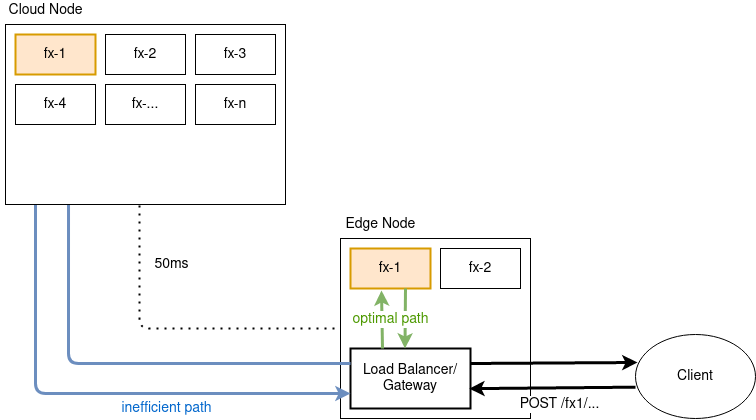
\includegraphics[width=12cm]{graphics/diagrams/efficient_path_example.png}
    \caption{Example diagram showing efficient and inefficient request routing based on network delay. "fx-1" through "fx-2" denote different types of function, and the dotted line denotes a network link between the cloud and edge node with a latency of 50ms}
    \label{fig:efficient_path}
\end{figure}

As can be understood quite intuitively in Figure \ref{fig:efficient_path}, round robin load balancing will in many cases lead to clearly suboptimal choices in terms of incurred network delay. The figure also shows the three key components we consider when trying to make network location based decisions: The client, the load balancer, and the node. Because our approach solely considers application level load balancers, since serverless platforms typically require these for their advanced routing decisions, any given request takes a path from the client to the load balancer, then to the selected upstream node, and back the same way.

Subsequently we want to incur the minimal amount of delay possible from both the hop between the client and load balancer, as well as between the load balancer and upstream node. Our proposed approach handles these two kinds of hops separately, at least for the most part. Since the scope of this work does not include optimizing the location of the serverless function instances themselves, this means we can improve performance through the following methods:
\begin{enumerate}
    \item \textbf{Intelligent load balancing decisions:} load balancers should choose upstream nodes that are both close in the network, and have \glspl{fet} short enough as not to negate the performance won through network proximity
    \item \textbf{Effective placement of load balancers:} the scheduler of the serverless system should place load balancers at locations in the network where they are in close proximity to clients and serverless function instances requested by these clients
    \item \textbf{Efficient scaling of load balancers:} the amount of load balancers should be high enough to provide the needed performance improvement, but not so high that the resources consumed by the load balancers diminish or even negate that effect
\end{enumerate}
In our approach the first method is provided by the load balancer itself. It is continuously updated with information where function instances, typically also referred to as \textit{replicas}, are located. Based on this and other information gathered by the load balancer, it tries to make decisions that lead to faster overall request responsiveness by selecting upstreams that are close and provide fast \glspl{fet}.

The other two methods are handled by the osmotic joint scaling and scheduling component of our approach. While the different methods of improvement are split between these two components of our proposed solution, this does not mean that they are completely separate from each other. Naturally the scheduling and scaling decisions will influence the way in which the placed load balancers work, while these in-turn affect the data gathered for and available to the scaling and scheduling component. The specifics of these two components will be discussed in the next two sections. 

It is also important to note that a significant amount of the approaches' implementation details are not chosen arbitrarily, but are rather the result of continuous cycle of experimentation and evaluation. While not detailed in the approach, the evaluation, result, and discussion chapters of this thesis include some of these experiments, in particular those that give additional insight into the problem domain and yielded results useful beyond informing this specific approach.
% Target: 8 pages with figures
\section{Least Response Time Load Balancing}
In this section we describe the role the load balancer plays in the context of our approach, how it is related to the underlying serverless platform, and the details of how it is implemented.

\subsection{Load Balancing Concepts}
While load balancing might at first appear as a rather simple problem, venturing outside cloud-centric scenarios, where resource homogeneity can be assumed, makes it much more complex of a challenge.
Since we feel the changes implied by resource heterogeneity are often only implicitly covered in literature, or an understanding of the problem is assumed, we believe that it is beneficial to describe it in more detail. This not only helps form a basis on which subsequent research can build, but also gives a lot of contextual information on how our approach relates to the underlying formal problem.

For our formulation of the load balancing problem we consider two types of resources: nodes, and network links. Nodes are the compute nodes in the cluster, and are characterized by the compute capabilities they possess and the function instances they host. Network links are characterized by their latency, and their bandwidth.
\begin{figure}
    \centering
    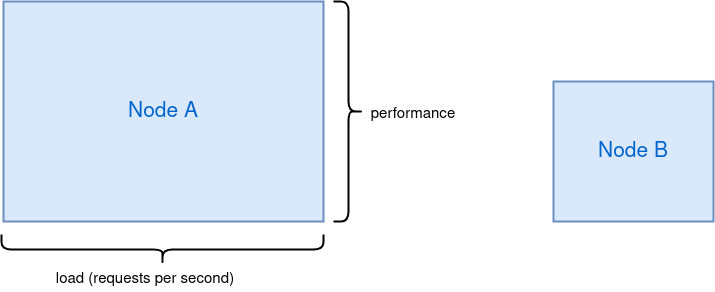
\includegraphics[width=12cm]{graphics/diagrams/load_balancer_squares.png}
    \caption{Rectangles representing a resource in our problem visualization}
    \label{fig:lb_squares_basic}
\end{figure}
To get a more intuitive understanding of the problem we developed a visualization, where resources are depicted as rectangles, where their dimensions correspond to their characterizing attributes. Figure \ref{fig:lb_squares_basic} shows an example of this. The width of the rectangle corresponds to the \textit{load} of the system, in our case measured in \gls{rps}, and the height corresponds to the performance, which since we are concerned about response times is the response time in milliseconds. One should note that, even though maybe counter intuitive, a greater height corresponds to higher performance, which in turn means \textit{lower} response times.
A core concept of this visualization is the capability of resources to \textit{stretch} or \textit{compress}. This means increasing or decreasing width or height of the resource, while doing the inverse to the other side. The condition is that the total area of the resource, i.e. the product of width and height, must be consistent throughout this process. This is effectively the way in which performance regression is modeled in this visualization, but one should not that this way only works under the condition that performance regression is linear with respect to the load. Luckily this is close to observed real world behaviour, %todo cite this
meaning that at least for understanding the underlying problem this visualization holds.
There are, however, limits to this stretching or compressing resources. From a visual perspective there is a bounding box around each resource, which cannot be exceeded in either height or width. This corresponds to the real world behaviour of workloads not getting faster beyond a certain point, even if resources would be available one one side, and requests simply timing out once responses exceed a certain time limit.
\begin{figure}
    \centering
    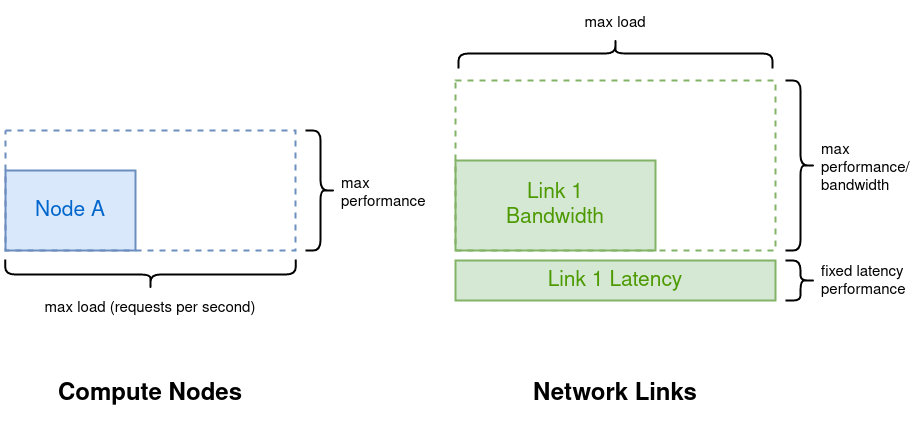
\includegraphics[width=14cm]{graphics/diagrams/lb_squares_real.png}
    \caption{Rectangles representing Node and Network Link resources, including their respective bounding boxes showing maximum load and performance capabilities}
    \label{fig:lb_squares_real}
\end{figure}
Network link resources work slightly differently, as they have a fixed component, dictated by the latency of the link, and a variable component set by the bandwidth. The variable component works as just described, while the static component is constant. Figure \ref{fig:lb_squares_real} shows the variable and static components along with their limits.

Resources can be conditionally linked. This maps the real world conditions of nodes being attached to the cluster via network links. Just like in actual clusters multiple nodes can be dependent on the same network link, and network links in turn can depend on another network link. 

\begin{figure}
    \centering
    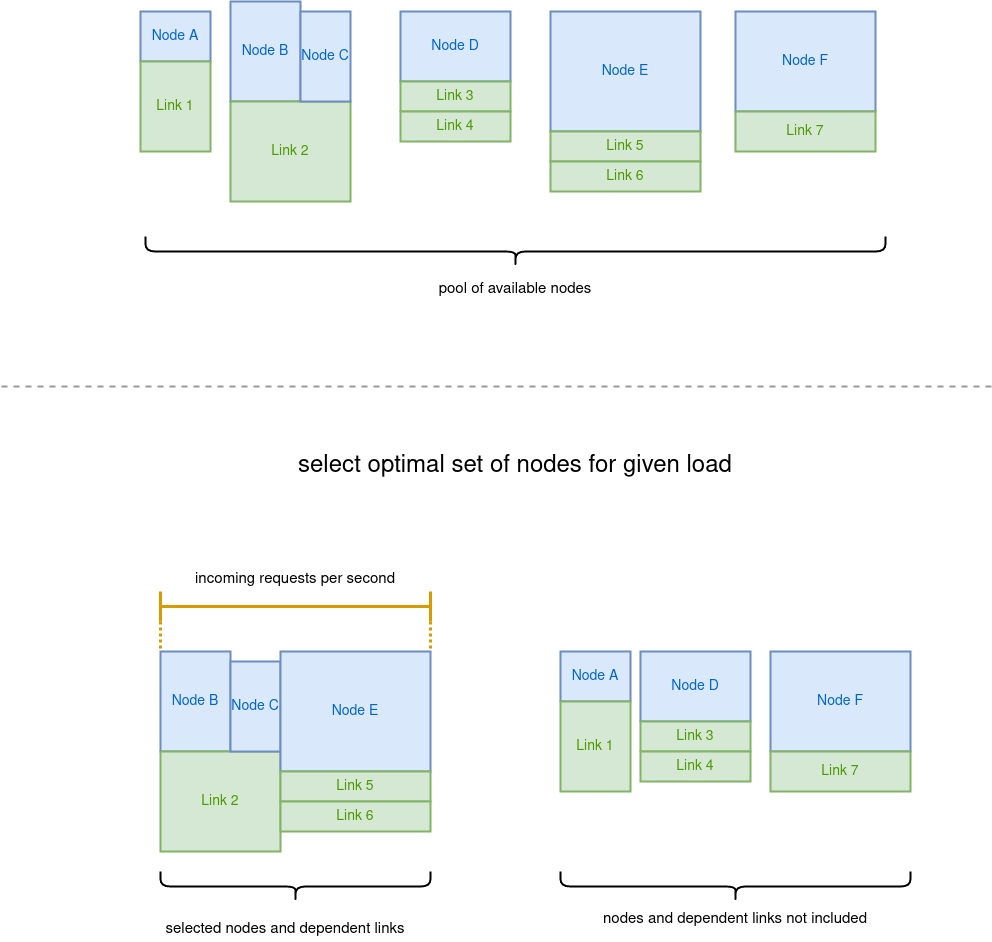
\includegraphics[width=14cm]{graphics/diagrams/lb_optimal_selection.png}
    \caption{Example visualization of an optimal selection of nodes, including their network links, for a given request load. Bounding boxes showing min/max load/performance, and fixed network latency performance parts are not displayed to keep the example simple.}
    \label{fig:lb_optimal_load}
\end{figure}

With this definition we can define the optimization problem an effective edge load balancer is trying to solve. The input to this problem is the given request load arriving from clients. In our visualization his corresponds to a set width. The objective is then to select nodes which when combined have the same width as the incoming client node, while at the same time maximizing the area of the nodes and network links selected. One needs to keep in mind that network links are not selected directly, but are implicitly included if selected nodes depend on them. Figure \ref{fig:lb_optimal_load} shows an example of such an optimal selection.

If the area is maximized in this optimization problem, response time is minimized, which is the goal a load balancer is trying to achieve.


While this visualization and problem is still relatively straightforward, there are other significant factors that we omitted until now:
\begin{enumerate}
    \item There are multiple functions, meaning that there are multiple "widths" or bins that need to be filled
    \item Functions share compute capabilities of nodes, meaning that performance regression, i.e. stretching and compression, needs to be considered over all functions running on a node
    \item Dependencies between network links and nodes aren't necessarily known
    \item Some network links necessarily handle traffic from outside the system, making performance regression assessment harder
    \item Actual performance profiles, i.e. dimensions, of nodes and functions aren't known
    \item Performance profiles, capabilities, client load, and function deployments change dynamically over time
\end{enumerate}

Considering these factors, load balancing in this context is a much higher-dimensional and thus more complex problem, where it is intuitively not clear whether an optimal solution is possible or if explicitly pursuing it in practise is even computationally feasible.


Since the true performance and regression characteristics of the nodes and network links are unknown, a load balancing solution needs to consider how this lack of information can be addressed. 
The simplest way to gather this information is by sending requests to nodes and observing response times. While this can yield insight into performance characteristics, these observations are merely a statistical sample, making them at least somewhat prone to misinterpretation. Especially when it comes to more complex behaviours such as functions sharing compute resources of nodes, or multiple nodes sharing network links.

Depending on the goals of the load balancer there is a risk/reward dynamic at play when it comes to sending requests to nodes in order to learn more about their performance characteristics. On one hand this can lead to "discovering" nodes that offer high performance and are able to handle a large number of requests, but on the other hand it could also lead to poor performance for those very requests in case network or compute capabilities are sub par.
There is no single correct answer to this dilemma, since the efficacy of any given solution would depend on the specific goals and tolerances of the application in question. In case \glspl{sla} exist that stipulate a certain response time for a minimum percentage of requests the risks might outweigh potential rewards, while an application that is somewhat tolerant to a fraction of requests being slow might experience a great performance uplift overall.
For our approach we consider \glspl{sla} to be out of scope, and therefore do not further address ways to address them. At the same time we want to point out that these are potentially relevant aspects for bringing serverless edge computing towards production readiness in the industry, and therefore highlight the areas where further study is needed.

\begin{figure}
    \centering
    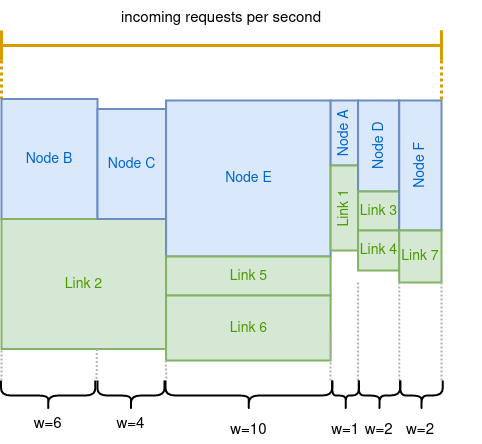
\includegraphics[width=10cm]{graphics/diagrams/lb_weights.png}
    \caption{Our approach as seen through the described visualization. All nodes are included in the "solution", and their load is determined by the load balancer assigning weights}
    \label{fig:lb_weights}
\end{figure}

Considering the myriad of potentially complicating factors for load balancing, in particular if one were to attempt to directly model the problem algorithmically, we decided to take a comparatively simple approach for our load balancing method.
In our approach we base our load balancing decisions solely on the total response time as it is observed by the load balancer. This means that we do not differentiate between times incurred from \gls{fet} and the times incurred from the networking portion. In this way we treat the total response time as a \textit{black box metric} to the overall system.
Our approach is to always include every single node in the "solution" to selecting appropriate nodes for the given width. This means that over the long term our approach gathers information about every potential node for every function replica that gets requested.
The disadvantage of this approach is that it dispatches requests to nodes that would not be included in a mathematically optimal solution, meaning that is will never reach the optimal performance possible assuming perfect knowledge of the system.
To counteract the performance penalty of including all nodes in the solution we assign them weights based on the response time they achieve.
This allows the load balancer to strike a balance between gathering information about the performance of the nodes available to the cluster, and processing requests as fast as possible.
Figure \ref{fig:lb_weights} shows the view of our approach on the system as described in the visualization. Note that the networking portion is not present, as our approach only considers the total response time in relation to the node it was sent to. Our approach also views each function replica separately, meaning that joint performance degradation of co-located function replicas is not modeled explicitly, only implicitly via the degraded performance observable through total request response times on that node.

There are a number of important considerations about the practical realization of our approach, which we will discussed next.


\subsection{Implementation}
As was just outlined our approach uses the response time as a black box metric to get insights into the system, and thus make load balanced decisions based on that information.
Since this basic idea does not constitute a concrete and testable approach we need to define the implementation details.

A well-known and simple implementation of this idea is the \textit{least response time} method of load balancing.
In this approach the server with the lowest average response time gets chosen whenever a request needs to be processed.
While this certainly works in general there are a few issues with this approach when it comes to serverless edge computing.
First, this approach can be problematic when it comes to co-located functions, as the load is not distributed among upstreams equally.
This leads to the fastest node being selected until its performance degrades enough for the next best node to be chosen.
Since there is no coordination that ensures some kind of balance, other functions that happen to be deployed on that node could experience severely hampered performance unexpectedly.
Second, this method does not take into account that the performance of nodes is, at least at first, unknown, and that it can change. A node that generally performs exceptionally well could be permanently excluded if at one point, for a spurious reason, performance was poor. A naive least response time load balancer would then likely rotate between a small handful of nodes that at one point performed well, effectively ignoring potentially better solutions.
These reasons point to the need of a more sophisticated approach than a naive implementation of least response time load balancing.

\subsubsection{Metrics Collection}
As explained, in our approach the metric used for load balancing decisions is the response time, specifically the time it takes between the load balancer forwarding the request to the selected upstream, and the load balancer receiving the response to the request.

Based on the response time data there are a number of performance metrics that could be calculated. Since our goal is to reduce the average total response time, we also chose the average response time as the key metric for load balancing decisions.
Depending on the requirements the load balancer needs to fulfill, other metrics could be used. A load balancer that is supposed to ensure a type of \gls{sla} might, for example, benefit from a percentile based metric instead.

In addition to effectively summarizing the performance of nodes, the metric needs to be time sensitive. Considering the performance of nodes can change over time, more recent values are more important as an indication of performance than those that lie farther back.
To address this, our approach makes use of a moving average with fixed window size.
We chose to use an exponential moving average since it has a number of advantages over more typical implementations.


\[\text{Given the previous average value } \mathbf{\bar{r}_{0}}\text{, the most recent response time } \mathbf{r}{,}\]
\[\text{the time passed since the last request }\mathbf{\Delta t} \text{, and the window size }\mathbf{w}\]
\[\text{The new average value }\mathbf{\bar{r}_{1}} \text{ is}\]
\[\bar{r}_{1} = (1 - e^{\frac{-\Delta t}{w}}) \cdot r + e^{\frac{-\Delta t}{w}} \cdot \bar{r}_{0}\]

The most significant advantage of this implementation over ones that use a buffer or a similar data structure, is precisely that complex data structures are not required. For each upstream only two values need to be recorded:
\begin{enumerate}
    \item The time the moving average was last updated
    \item The current value of the moving average itself
\end{enumerate}
While there are situations, where this can be less accurate, it is far easier to implement than buffer based solutions, since with these the required buffer size is unknown thus leading to frequent memory allocations and de-allocations.
Using an exponential moving average ensures minimal memory consumption, while at the same time being easy to understand and implement.

\subsubsection{Choosing Upstreams}
With the metrics collected what remains is deciding on upstreams based on those values. As previously outlined, naively choosing the upstream with the lowest average response time is potentially problematic.
For this reason our approach uses weighted round robin to decide which upstream should service a given request, where the response time metrics determine the weight assigned to each upstream.

The decision how exactly this weighted round robin gets implemented is surprisingly important, since the load balancing decisions affect the accuracy and volume of performance data gathered on each node, thus creating a feedback cycle that can, depending on the situation, lead to sub optimal performance.
For our approach we decided to use the same method employed by NGINX\cite{nginx}, a popular web-server and request proxy.
We chose this approach after experimenting with other solutions, and analyzing their performance profiles and characteristics with regard to the unique challenges posed by serverless edge computing environments.
Compared to other approaches is has the advantage of being deterministic, leading to all nodes being chosen eventually, which gives the load balancer sufficient data to make informed decisions, while at the same time distributing traffic in a mixed fashion between upstreams of different weights.
The evaluation methodology and experiment results of these experiments can be found alongside the general evaluation in the subsequent chapters.

\begin{algorithm}
  \KwIn{Set of available nodes $n_{0},n_{1},n_{...} \in N$}
  \KwIn{Weights for each of the nodes $w_{n_{0}}, w_{n_{1}}, ... \in W$}
  \KwIn{Current counter value for each node. $c_{n_{0}}, c_{n_{0}}, ... \in C$}
  \KwOut{The node the next request should go to}
    \For{$n \in N$}
    {
        $c_{n} \leftarrow c_{n} + w_{n}$ \Comment{add node weight to its counter}
    }
    $\text{selectedNode} \leftarrow n: c_{n} = max\{c: c \in C\}$ \Comment{select node with highest counter value}\\
    $c_{\text{selectedNode}} \leftarrow c_{\text{selectedNode}} - \sum_{w \in W}w$\\
    
  \Return{selectedNode}

  \caption{Smooth Weighted Round Robin}
  \label{alg:smooth-wrr}
\end{algorithm}
%todo: maybe rework this to be a bit more elegant
% currently a bit too much of a mashup between, math, set theory, code

\begin{table}[]
\centering
\begin{tabular}{llll}
Node          & \textbf{A}                & \textbf{B}                & \textbf{C}                \\
Weight        & \textbf{4}                & \textbf{2}                & \textbf{1}                \\ \hline
Iteration \#1 & \cellcolor[HTML]{FFCE93}4 & 2                         & 1                         \\
              & -3                        & 2                         & 1                         \\ \hline
Iteration \#2 & 1                         & \cellcolor[HTML]{FFCE93}4 & 2                         \\
              & 1                         & -3                        & 2                         \\ \hline
Iteration \#3 & \cellcolor[HTML]{FFCE93}5 & -1                        & 3                         \\
              & -2                        & -1                        & 3                         \\ \hline
Iteration \#4 & 2                         & 1                         & \cellcolor[HTML]{FFCE93}4 \\
              & 2                         & 1                         & -3                        \\ \hline
Iteration \#5 & \cellcolor[HTML]{FFCE93}6 & 3                         & -2                        \\
              & -1                        & 3                         & -2                        \\ \hline
Iteration \#6 & 3                         & \cellcolor[HTML]{FFCE93}5 & -1                        \\
              & 3                         & -2                        & -1                        \\ \hline
Iteration \#7 & \cellcolor[HTML]{FFCE93}7 & 0                         & 0                         \\
              & 0                         & 0                         & 0                        
\end{tabular}
\caption{An example of weighted round robin iteration results when using Algorithm \ref{alg:smooth-wrr} as we do in our approach. Colored cells indicate the selected node at the iteration.}
\label{tab:smooth-wrr-demo}
\end{table}

Algorithm \ref{alg:smooth-wrr} shows a pseudo-code implementation of our weighted round robin component using the approach also used in the NGINX source code \cite{nginx-wrr}.
Table \ref{tab:smooth-wrr-demo} shows how this implementation of weighted round robin distributes requests between upstreams of different weights. Note that the proportions between the weights are considered when choosing upstreams without using a fixed ordering based on weight, meaning that choices of upstreams with lower weights are interleaved between choices of upstreams with higher weights. %todo rewrite this. It's super unclear what is meant by this.

The only part of our load balancing approach that is not yet described is how the average response time recorded is mapped to the weight used by our weighted round robin implementation.
There are a number of ways in which values like this can get mapped to weights.
There is, unfortunately, no single correct answer since the lack of precise information on the state and performance of nodes and the network prevents us from reliably making globally optimal load balancing decisions.
There are two factors that determine how response times are mapped to weights:
\begin{enumerate}
    \item The weight range response times should be mapped to
    \item The function by which they are mapped to these weights
\end{enumerate}

In our approach we chose to use a fixed range of weights, since this makes sure every upstream is assigned at least a fixed fraction of traffic.
This guarantees that the response times of all upstreams are sampled eventually, preventing a situation where a significant change in the performance of an upstream goes unnoticed forever.
The weight of each upstream is determined by it's average response time in the last value and calculated using the following formula:
\[ \text{Let } \bar{r} \in R \text{ be the set of response time averages, and }\]
\[ w_{\text{min}} \text{ the minimum weight, } w_{\text{max}} \text{ the maximum weight, then}\]
\[ \text{the weight for each response time average } w(\bar{r})\text{ is defined as}\]
\[ w(\bar{r}) = max\{w_{\text{min}}, \frac{w_{\text{max}}}{(\frac{\bar{r}}{min\{\bar{r}: \bar{r} \in R\}})^{s}}\} \]
\[ \text{where } s > 0\text{ is a chosen scaling factor }\]

The scaling factor determines how weights correlate to response time. A scaling factor of 1 means that there is a linear relationship between the average performance and the weight.
Figure \ref{fig:weight_mapping_example} shows the effect different scaling factors have on weight mappings in the weight range of 1-10. Both continuous and integer values are shown, since it depends on the weighted round robin implementation which of the two can be used.
Based on grid-search experiments we chose a weight range of 1-25, and a scaling factor of 2. (//note to me: these experiments should be expanded a bit and values updated if necessary).
The experiments that determined this choice will be described in detail in subsequent chapters.

% idea: factor (i.e. deciding on linearity) depends on how strong the link between performance and capacity is. i.e. if strong performance means high capacity, we can assign super high relative weights. Is this even important? Since on paper overload etc. should eventually lead to a balance being achieved, no?
% idea: spread (i.e. size of weight range) depends on how dynamic the system is and how high we value information gain, since high spread -> more optimal in static condition. low spread -> discovers changes faster in dynamic conditions.

\begin{figure}
    \centering
    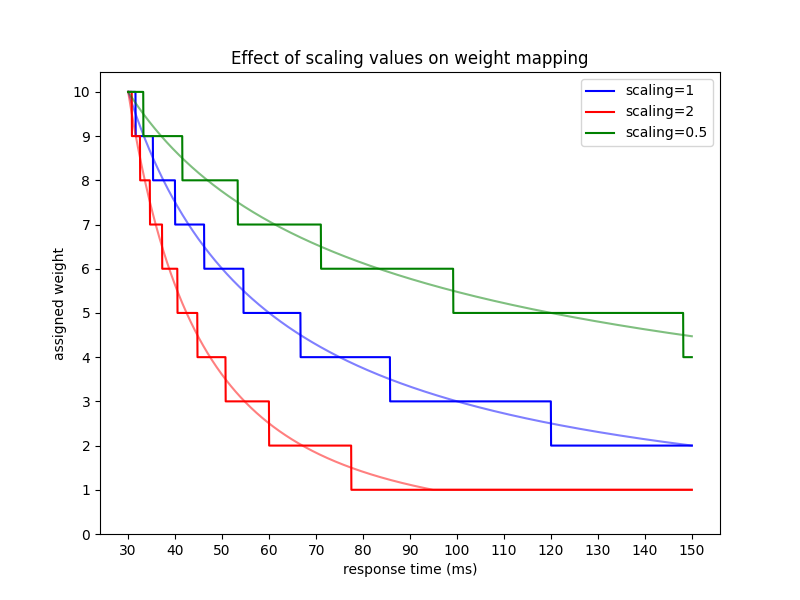
\includegraphics[width=10cm]{graphics/graphs/weight_mapping_scaling_example.png}
    \caption{Plot showing the effects of different scaling factors on how response time averages are mapped to weights.}
    \label{fig:weight_mapping_example}
\end{figure}


\subsubsection{Framework Integration}
In our approach the load balancers are assumed to be integrated into the serverless framework.
This means that load balancers are notified of changes to function replicas, meaning that they are always aware which functions exist, and which exact replicas are available for each function.
From a practical perspective this is simple to achieve in a production implementation as serverless frameworks already provide this information in some way, and the underlying technologies, typically some kind of container orchestration, also have means to retrieve the necessary data.

Apart from the available functions and their respective replicas, new load balancer instances are initialized with response time values and weights of already running load balancer instances nearby.
While the load balancer still needs to adapt its weights based on its specific client load and position in the network, this initial pre-loading of values allows it to converge on a stable configuration faster, thus resulting in quicker performance gains.


% Target: 8 pages with figures
\section{Osmotic Scaling and Scheduling}
In this section we describe our approach to scaling, and scheduling load balancer replicas, meaning the process by which we decide how many load balancer instances are in the system, and on which nodes they are placed.

\subsection{Osmotic scaler and scheduler}
To determine the number of replicas and their location we opted for an approach based on \textit{osmotic pressure}.
Like we outlined in previous chapters, osmotic pressure is a high level concept supposed to facilitate elastic diffusion, elastic diffusion being the process by which a central starting configuration, typically in the cloud, is extended to the edge dynamically based on request load with the goal of providing low latency communication for edge clients\cite{osmotic-middleware-rausch}. 
The general idea of this approach is that client requests generate pressure on nodes that are close to the clients, meaning that they could potentially host a load balancer instance, and then using this pressure in conjunction with a set threshold to determine both the number of load balancer instances and their locations.
If pressure at a node exceeds a certain level, because there are a lot of client requests originating close by, a load balancer will the, be placed at the node, thus lowering the pressure.
Conceptually this approach is supposed to create an equilibrium of pressure throughout the system, which results in a well-chosen set of load balancer instances.
This means that by using an osmotic approach, the scaling and scheduling decisions are effectively made together and cannot be controlled separately.

The main challenge of realizing an approach based on the concept of osmotic pressure is finding the method by which pressure is calculated. This can be particularly challenging when the system requires a manually set pressure threshold, since this requires the threshold value to fulfill a number of criteria:
\begin{enumerate}
    \item \textbf{Intuitive:} the threshold value should be at least somewhat intuitive to whoever determines it. It should be clear what a certain pressure threshold \textit{means}, and how it will affect the system.
    \item \textbf{Robustness:} the threshold should be reasonably robust to dynamically changing systems. A few extreme outliers in the system, for example extremely far or close nodes, should not require the threshold to be changed to still achieve the desired behaviour.
    \item \textbf{Linearity:} while not necessarily fully achievable, ideally changes in the threshold value should have a close to linear relationship with the scaling and scheduling behaviour. This is important in conjunction with its intuitiveness and is important to prevent sudden, unexpected effects such as dramatically changed system behaviour with minuscule changes in the threshold value.
\end{enumerate}

\subsection{Calculating osmotic pressure}
Building on the previously outlined requirements we can develop a pressure calculation methodology.
\subsubsection{Required data}
Because osmotic pressure based scaling and scheduling is at its core still a heuristic-driven approach, we cannot assume to have perfect global knowledge of the system.
Our approach is built with that in mind, staying close to assumptions about data availability already used for the load balancers themselves, and building on information current container orchestration platforms such as Kubernetes already provide.
For our calculation of osmotic pressure we require the following data:
\begin{itemize}
    \item Network locations of all function replicas, i.e. which nodes the instances are running on
    \item Network locations of all clients
    \item Number of all client requests, and which functions they are for
    \item Network locations of all load balancer replicas
    \item Network distances (latency) between nodes and clients
\end{itemize}
Replica information is readily available through state of the art container orchestration platforms, while network distances and exact client request numbers are relatively simple to obtain.
Because of this comparatively available set of data, we believe that our approach could easily be integrated into current serverless frameworks.
\subsubsection{Concept}
The basis of our pressure calculation is a hypothetical "what-if" scenario.
For all nodes in the system that could potentially host a load balancer, and are currently not doing so, we ask the question "what if there was a load balancer instance running on that node".
We then compare this hypothetical scenario to the current state of the system and determine whether the hypothetical addition of the load balancer on the node would constitute an improvement or deterioration in performance, and if so by how much.
For nodes that are hosting a load balancer already we do the same in reverse and ask "what if there wasn't a load balancer there", once again estimating whether performance would improve or deteriorate.

The two metrics we use to determine the impact of adding or removing load balancer replicas are the \textit{request share} and the \textbf{projected performance} of the node.
These metrics are calculated for each node on a per-function basis, and ultimately determine the pressure.

\subsubsection{Request Share}
\begin{figure}
    \centering
    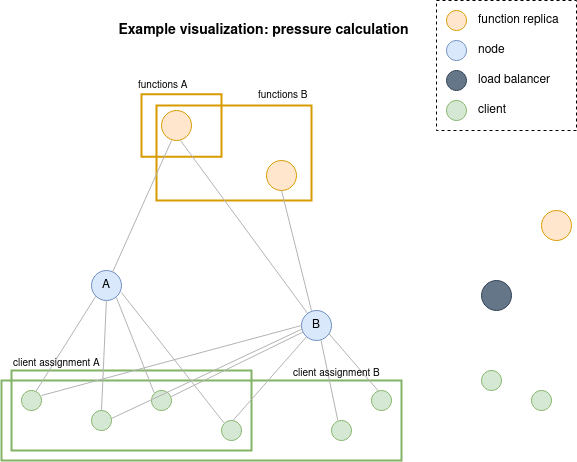
\includegraphics[width=12cm]{graphics/diagrams/client_lb_assignment.png}
    \caption{Assignment of clients and function replicas to potential load balancer nodes during pressure calculation}
    \label{fig:cl_lb_assignment}
\end{figure}
The request share is one of the central metrics we use to determine a node's pressure. In principle it shows which portion of the system's total incoming requests would be routed over that node, if it had a load balancer.
To calculate this value we need to first look at client assignment, meaning the process by which it is determined which client will send requests to which load balancer.

As we already outlined previously, one of our core assumptions is that clients will send their requests to whichever load balancer is closest from a network perspective, which is the load balancer with the shortest \gls{rtt}.
In keeping with our hypothetical scenario of "what if there was a load balancer on this node", clients will send their requests to this potential new load balancer if that node is closer to the clients than whichever load balancer instance is currently closest.
An example visualization of this client assignment for calculating request share can be seen in Figure \ref{fig:cl_lb_assignment}.
The specific number of clients our potential load balancer would service is, however, only of secondary importance. The more important and precise metric is the number of requests it will service.
We do not really care about whether there are a lot of clients sending few requests, or a low number of clients sending a large amount. What is important is only the number of requests going to the potential load balancer relative to the total amount sent.
Generally the data for this calculation is readily available, and can easily be gathered for example via existing load balancers reporting on the requests they receive.

A point to note here is that we only consider the requests sent within a certain time frame for this calculations, as they should be recent enough to be relevant for current scaling and scheduling decisions.
In our case we chose this time frame to be the last 60 seconds, which is relatively short but works within the relatively dynamic and heterogeneous systems we consider.
For real deployments this value might have to be adapted based on how dynamically the request load changes, how many requests each client typically sends in a session, and what amount of load is generally typical of the system.
The important point to consider here is that the time frame needs to be long enough to give a reasonably accurate picture, while not being so long that the data is delivers is not reflecting the current state of the system anymore.

Lastly, since there are multiple functions in the system, which we generally consider to be of equal importance, we calculate the request share the potential load balancer would receive on a per-function basis.
Thus we define the \textit{request share} as the following:
\[ \text{Let }N\text{ be the set of nodes,} \]
\[ L\text{ the set of nodes with running load balancer instances,} \]
\[ F\text{ the set of serverless functions,} \]
\[ \text{and }C\text{ the set of clients.} \]
\[ \text{Further let } dist(n,c) \text{ be the distance between a node } n \in N \text{ and client }c \in C\text{,}\]
\[ \text{ and let }requests(c, f) \text{ be the number of requests from client }c \in C \text{ for function }f \in F\]
\[ \text{Then for each node }n \in N\text{ the assigned clients are defined as} \]
\[ assignment(n) = \{c | c \in C \land dist(c,n) < min\{dist(l, c) | l \in L\}\}\]
\[ \text{Finally the request share for node } n \in N \text{ for function }f \in F \text{ is defined as } \]
\[ rqshare(n,f) = \frac{\sum_{c \in assignment(n)}requests(c,f)}{\sum_{c \in C}requests(c,f)}\]
Thus we define the request share of a node for a given function, as the fraction of all requests for that function the node would receive if it had a load balancer instance running.
\subsubsection{Projected Performance}
The second major metric that determines the pressure of a given node is what we refer to as the \textit{projected performance}.
This metric is once again based on the hypothetical scenario of "what if there was a load balancer on the given node" and is supposed to estimate the level of network performance we could expect if a load balancer is actually placed there.
Conceptually our notion of performance is rather simple.
It is determined by how close the clients are that would be assigned to that node, and by how close the function replicas are.
We once again calculate this metric for each node, and on a per-function basis.
To calculate the \textit{client distance} we use the average distance of all assigned clients, weighted by their relative share of requests among the assigned clients for the given function.

The calculation of the \textit{function distance} is somewhat more intricate.
Using a flat average over all function replicas is not a particularly suitable metric, since this would also consider the distance of function replicas that are far away, meaning that we would include the distance to function replicas we don't want the requests being sent to in the first place.
To address this issue we only consider a subsection of function replicas to calculate the function distance.
Our approach to the function distance is based on the assumption that the function scaling component correctly scales the function as required, meaning that we assume that the total number of function replicas is sufficient to serve the given number of incoming requests.
The number of function replicas we consider for a node is based on that nodes request share. We take into account the fraction of closest function replicas equal to the request share of the node for which we want to calculate the function distance.
If a node, for example, has a request share of 0.5, meaning 50\%, then its function distance is the average distance of the 50\% closest function replicas.
An example of this can once again be seen in Figure \ref{fig:cl_lb_assignment}, where nodes A and B have a differently sized share of functions assigned to them for distance calculation based on their respective request share.
Since we assume that the function replica scale is sufficient to handle the systems requests, this should mean that, not accounting for heterogeneity in function replica performance, the replicas considered for the function closeness metric are sufficient the incoming requests of the load balancer.
The reason we are not considering heterogeneity in replica performance is that this factor is not known beforehand, and in addition hard to estimate.
Finally we add the function distance and client distance together and invert them, since our subsequent calculations require the projected performance metric to have high values indicating good performance, and low values indicating poor performance.
Making this explicit we arrive at the following formulation for our projected performance:
\[\text{Let } replicas(f) \text{ be the set of replicas of a function }f \in F\]
\[\text{Then the client distance for a function }f \in F \text{ and node }n \in N \text{ is}\]
\[cldist(n,f) = \frac{\sum_{c \in assignment(n)}dist(n,c) \cdot requests(c,f)}{\sum_{c \in assignment(n)}requests(c,f)} \]
\[\text{Let }repdist_{n,f} = \langle r_{0}, r_{1}, ... \rangle \text{ be the list of replicas for a function }f \in F \text{ ordered by} \]
\[\text{their distance to }n \in N \text{ in ascending order such that for each pair } \]
\[(r_{i},r_{j}) \in repdist_{n,f}^{2}: i < j \implies dist(n, r_{i}) \leq dist(n, r_{j})\]
\[\text{Then the set of replicas considered is } \]
\[replicas(n,f) = \{r_{i} | r_{i} \in repdist_{n,f} \land i < \lfloor rqshare(n,f) \cdot |repdist_{n,r}| \rfloor\}\]
\[\text{Thus the function distance is }fndist(n,f) = \frac{\sum_{r \in replicas(n,f)}dist(n,f)}{|replicas(n,f)|} \]
\[\text{Finally the projected performance is }perf(n,f) = \frac{1}{cldist(n,f) + fndist(n,f)} \]
Needless to say slight adaptations of these formulas are necessary for a practical implementation.
For our simulator based evaluation the formulas are used exactly as we present them here, with the exception that special values are used as placeholders for undefined values, particularly those that result from a division by 0.
If a node has a request share of 0 for example, the projected performance is simply set to 0.
Likewise if the request share is > 0, the function distance calculation will take into account at least one replica, even if based on these formulas none would qualify.


\subsubsection{Pressure}
Now that we defined request shares and the projected performance we can move on to the actual pressure calculation.
In our approach we calculate what we call \textit{relative pressure}.
This means that the pressure of a given node is always in relation to the current state of the system, and not in absolutes.
This is done to ensure that the pressure calculation is not dependent on a-priori knowledge of the system.
If, for example, pressure were directly related to the number of requests per second the user would have to define what number of requests is considered high or low manually beforehand, negating precisely the kinds of advantage serverless frameworks are supposed to afford: Alleviating developers from complex configuration.

Our proposed notion of pressure is focused on the changes adding a load balancer on the node in question would bring to the system.
We start out by making an estimation of the average performance and impact of a load balancer in the system.
This notion of performance is based on the already described projected performance, and the load balancers request share.
We cannot rely purely on the projected performance, as it is also tremendously important for how many requests this performance is provided.
If we, for example, have a situation where we need to decide between two nodes which could potentially host a load balancer, that have a very high projected performance, then we most likely improve overall system performance more by selecting the node with the higher request share, since the high expected performance will affect more requests.

We call our estimation of the current system performance the \textit{status quo performance}.
To calculate it we once again rely on the projected performance, and the request share of node, although since we are interested in the current state of the system we consider these metrics only for nodes which currently host a load balancer.
The calculation of these metrics is exactly the same as for nodes that do not have load balancer instances deployed on them.
A slight difference to note is that the partition of clients onto nodes with load balancers will be without overlap, meaning that if we sum up all the request shares of a function over all nodes with a load balancer, the result would be 1, i.e. 100\%.

For our pressure metric this status quo performance is calculated using a weighted quantile.
The projected performance of the load balancer nodes are the values over which the quantile is calculated, while their respective request share is the weight.
We use the 50\% weighted quantile, also referred to as the weighted median, as our status quo performance.
In our testing the weighted median provided a robust metric that behaved predictably and similarly over different network topologies and cluster sizes.
It is, however, conceivable that there are situations in which this quantile should be set higher or lower depending on how dynamic the system changes, and how heterogeneous its structure and network topology are.
We should also note that at this point all of these metrics are still calculated on a per-function basis.
The values for each function are only combined at the very end, weighted by how important the individual functions are.
In our case the importance of individual functions is determined by which proportion of total requests are directed to it.
This means that we effectively treat each request as equally important and thus a function which gets double the traffic of another, for example, would also be considered twice as important when the individual function based metrics are combined.

% todo this should probably we rewritten a bit to be less repetitive
With this metric we can now calculate our pressure metric. For a given node we do this by calculating its impact on the system compared to the status quo performance.
Assuming that the status quo performance represents the current system performance overall, we compare the status quo performance with the performance of the system with the node added.
Since, as described earlier, the current set of load balancers services all client requests, adding a new load balancer will remove some of the traffic from existing load balancers.
This amount is represented by the potential load balancer node's request share.
To then calculate the system performance with the potential load balancer added we replace a part the size of the node's request share with the nodes performance.
Lastly we compare by how much adding a load balancer on this node changes the overall system performance, by calculating their difference in percent.
This percentage difference is the pressure value we use to make scaling and scheduling decisions in our osmotic system.
A positive pressure indicates that adding would likely improve performance, while negative pressure indicates that it would likely deteriorate overall system performance.
Thus we formally define our pressure as follows:
\[\text{For each function }f \in F \text{ it's relative importance is }\]
\[importance(f) = \frac{\sum_{c \in C}requests(c,f)}{\sum_{f' \in F}\sum_{c \in C}requests(c,f')} \]
\[\text{Let the set of tuples of a load balancer node's performance and request} \]
\[ \text{share for a function }f \in F \text{ be} \]
\[lbperf_{f} = \{(perf(l,f), rqshare(l,f)) | l \in L\} \]
\[\text{Then for a function the weighted median performance is } statusquo(f) = weightedmedian(lbperf_{f})\]
\[\text{Based on this we can estimate the system performance when adding a load balancer on node }n \in N\]
\[ addperf(n,f) = (rqshare(n,f) * perf(n,f)) + ((1 - rqshare(n,f)) * statusquo(f))\]
\[\text{which relative to the status quo performance gives us the pressure per function} \]
\[ fp(n, f) = \frac{addperf(n,f) - statusquo(f)}{statusquo(f)}\]
\[\text{Then combined the final pressure of the node is } p(n) = \sum_{f \in F}fp(n,f) \cdot importance(f)\]

\subsubsection{Downscaling Pressure}
Just like we need pressure to determine where load balancers should be scheduled, we also need to decide on conditions which trigger an existing load balancer to be removed.
Without this mechanic the osmotic scaling and scheduling component would not be able to properly adapt to changing system conditions, since load balancers that aren't placed effectively anymore cannot be removed.
During development we learned that an important property of the osmotic scaling and scheduling system is that it is consistent.
For our purposes this means that it should find a stable configuration eventually that doesn't change anymore unless the surrounding system parameters change.
In our testing the use of the exact same metric for removing load balancers as for adding them led to oscillations in their scheduling, meaning that there were cases were a load balancer would be added only to be removed again immediately.

To address this we use a slightly different measure of pressure for removing load balancer replicas.
It is also based on a hypothetical scenario, though in this case we try to estimate the consequences removing a load balancer would have on the system performance.
Compared to the pressure when adding load balancer replicas, we use a somewhat more accurate measure than for the removal process, since the original and future state of the system are more well known, considering it relies on more tangible and less hypothetical data.
First, the status quo before removal is calculated.
This is a weighted average of the projected performance of all load balancers weighted by their request share.
For the system performance once the load balancer is removed, we calculate how the system structure would change if the load balancer is removed.
The primary change this entails is that the removed load balancers clients would then send their requests to the next closest load balancer instance.
For simplicity and calculation efficiency, we assume that the clients would be assigned to whichever load balancer is closest to the one potentially getting removed.
At this point we recalculate the projected performance and request share of the load balancer that takes over the clients.
Based on this we can then calculate the system performance with the load balancer removed by again using a weighted average over the projected load balancer performances weighted by their request share, with the difference being that the load balancer we potentially remove is no longer counted, and its clients are moved to the next closest load balancer.
We then have an estimation of system performance with and without the load balancer in question, and go on to calculate their percentage difference.
This percentage difference tells us by how much removing the load balancer would affect overall system performance in percent, and based on a user defined threshold the scaler then decides to remove or keep each individual load balancer instance.
\[\text{For a function }f \in F \text{ the pre-removal status quo system performance is }\]
\[rmstatusquo(f) = \sum_{l \in L}perf(l,f) \cdot rqshare(l,f)\]
\[\text{If we then remove a load balancer }l \in L \text{ the clients are taken over by another load balancer} \]
\[l': dist(l,l') \leq min\{dist(l,l'') | l'' \in L \setminus \{l\}\} \implies assignment(l') = assignment(l') \cup assignment(l)\]
\[\text{Giving us the adapted set of load balancers }L' = L \setminus \{l\} \]
\[\text{Then the system performance without the load balancer for a function is} \]
\[rmperf(l,f) = \sum_{l' \in L'}perf(l',f) \cdot rqshare(l',f) \]
\[\text{Based on which we can calculate the removal pressure per function as}\]
\[ rmfp(l,f) = \frac{rmperf(l,f) - rmstatusquo(f)}{rmstatusquo(f)}\]
\[\text{and then combine them to the final removal pressure } rmp(l) = \sum_{f \in F}rmfp(l,f) \cdot importance(f)\]

\subsubsection{Throttled Scaling}
In our approach the scaling and scheduling components calculates pressures for all nodes and load balancers, and then makes subsequent scaling decisions, at a fixed interval.
While in theory multiple nodes could have a pressure beyond the set threshold that warrants adding a load balancer in a single interval, in our approach we artificially throttle this amount.
In our implementation of the scaling and scheduling component only a single load balancer can be added or removed per iteration.
We compensate for this comparatively slow rate of change by running the scaling and scheduling calculations at relatively short intervals.
There are two major reasons for our choice to limit the rate of change in the system in this way.

\begin{enumerate}
    \item The pressure metrics and calculation are based on the addition or removal of a single instance
    \item Since request shares potentially overlap, scheduling multiple load balancers often leads to immediate removal during the next scaling and scheduling cycle
\end{enumerate}

During development we observed faster convergence to a stable configuration when only adding or removing a single load balancer at a time.
We also considered changing our pressure calculations to optimize for a faster rate of change, but decided against it because these calculation are much less intuitive, which is detrimental to the ease of parametrization of the system, and most importantly the computational effort rises sharply with the number of load balancer instances that are considered simultaneously.
While the single node calculations we use only require calculating a maximum of 250 scenarios for a system with 250 nodes, the equivalent calculations for two nodes being scheduled simultaneously would require calculating up to 31125 scenarios for an equally sized system.
While this does limit the potential rate of change, we believe that a rate of change of about 4 load balancers per minute, which could still be increased if necessary, should be enough to handle the requirements of even comparatively dynamic systems.




% 10ish pages, about 8 in text, about 2 in figures
% Results had 18 pages, 50/50 ish split
% probably some 20ish pages here
\chapter{Evaluation}

% Stuff that goes here:
% Faas-sim: what is it, how does it work, what are its models, how does it deal with containers/kubernetes/openfaas/etc. What is simulated, what isn't? How are network flows simulated?
% Request pattern stuff.
% what types devices are there
% what functions are there, how do they perform on each device?
% image sizes, pulls, request payload sizes, all that stuff
% topologies: What are there and how are they built? real measurements from papers, etc. etc.
% -> city level, both old and modern, visualizations, etc.

% practical: how did we eval traefik
% real cluster, galileo (briefly), what devices are there? Auto-responder type app, payload size, response time, etc.

% Experiments:
% 1) Prelims
% 2) traefik resource eval
% 3) more realistic topo
% 4) load balancer count tests
% 5) LB hyperparameter tests
% 6) the osmotic stuffs?

\section{Initial Assessment}
% good 3-4 pages

\section{Load Balancer Implementation and Parametrization}
\section{Least Response Time Load Balancing Implementation}
% 2 pages
\section{Load Balancer Parametrization}
% with graphics 2 pages -> with graphics got 5-6 pages.
With this range of experiments we set out to better understand the effects different parameters have on a load balancers performance.
We then continue to use this information to make an informed decision for the load balancer parameters in subsequent experiments.

Specifically, we want to understand the relationship between the following load balancer parameters:
\begin{enumerate}
    \item \textbf{Scaling Factor:} the factor which determines how linearly observed node performance is mapped to weights
    \item \textbf{Weight Range:} the size of the weight range the load balancer can use
    \item \textbf{Current Weight Reset:} whether or not it makes sense to reset the current weights of the load balancers when the weights are changed
\end{enumerate}

\subsection{Setup}

Since previous experiments have shown that the impact parameter changes can have are at times hard to predict, we decided to perform this evaluation using a grid-search, meaning that we rely on trying a large number of permutations to find patterns in their behaviour.
To test these settings we do not rely on the full FaaS-Sim environment, but rather perform isolated tests with a single load balancer and less sophisticated function and network simulations.

Since we are trying to evaluate how well load balancers choose upstreams, the upstreams are the comparatively most accurately simulated component.
The performance model of our simulated upstreams is closely informed by our notion of a node's performance level and capacity, which we outlined in our load balancing approach.
Thus, each simulated upstream has a set level of performance, which determines how long it takes for a request to be processed.
Since our aim is to keep this simulation simple, we consider the response time determined by the upstream to represent both the network and the \gls{fet} that would be observed in a real serverless system.
Each upstream samples its response times from a set of two lognormal distribution, one of which represents the \gls{fet}, while the other represents the network time.
To simulate the effect of high load, each upstream also has a set capacity, measured in requests per second.
If an upstream receives more requests per second than is has capacity for, \glspl{fet} start to degrade linearly, meaning that response times get longer in proportion to how overloaded the upstream is.

To represent different system conditions we introduce \textit{performance spread} as an input variable to these experiments that determines the how heterogeneous the performance of the simulated upstreams is.
The assumed system scenario is closely aligned with the one of our initial evaluation.
Relative to the load balancer a node can fall into one of four location categories, which determine the network distance from the load balancer: \textit{local}, \textit{city}, \textit{nation}, and \textit{global}.
Like it would  be in a real scenario, the probabilities of nodes falling into each of the categories gets progressively higher, meaning that a very low number of nodes will be local, while the majority will be \textit{global} and thus rather far away form a network perspective.
Apart from their location, nodes can fall into three performance categories, which are \textit{small}, \textit{medium}, and \textit{large}.
This performance category determines both the typical \gls{fet} of that node and its capacity.
Small and medium nodes are more likely to be located close to the load balancer, while large nodes are likely to be farther away in the network.
This is done to represent a typical edge computing scenario where relatively weaker compute is available locally, with a large amount available farther away, e.g. in the cloud.
The performance spread then determines how big the differences between the different categories nodes can fall into are.
A performance spread of 15 for example would correspond to as scenario where \glspl{fet} range from 10ms to 150ms, capacities from 5\gls{rps} to 100\gls{rps}, and network times from 5ms to 250ms.
A higher performance spread would indicate higher performance differences, while a lower one would indicate lower differences, with a performance spread of 1 indicating complete homogeneity.


To make an informed decision on load balancer parametrization we performed three experiments.
\subsubsection{Scaling Factor and Performance Spread}
In this evaluation we examine the effect the scaling factor has on performance in a variety of different scenarios.
To this end we tested scaling factors from 0,1 to 10.
Scenarios included performance spreads from 1 to 46, and all scenarios were repeated three times with request loads of 50\gls{rps}, 250\gls{rps}, and 1000\gls{rps}.
The weight range upstreams were mapped onto in this experiment is [1;10].
The experiment covers a simulated time frame of 1000 seconds.

\begin{figure}
    \centering
    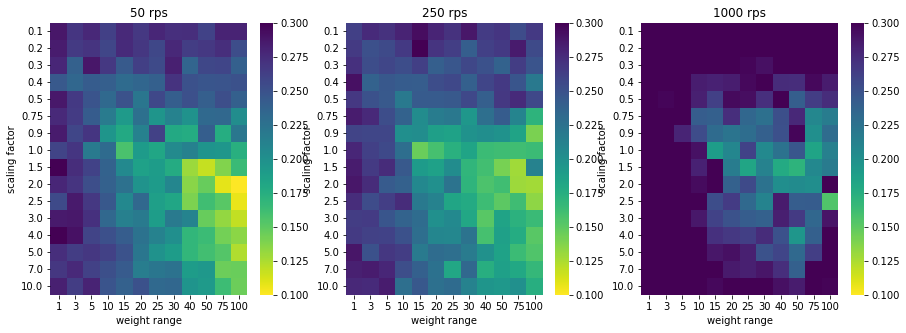
\includegraphics[width=14cm]{graphics/graphs/lb_hyper_scaling_vs_performance_spread.png}
    \caption{Mean response time over various levels of performance spread and scaling factors}
    \label{fig:lb_hyper_scaling_perfspread}
\end{figure}

The results of this experiment can be seen in Figure \ref{fig:lb_hyper_scaling_perfspread}.
Aside from showing lower performance for higher performance spreads, which is entirely to be expected since a larger performance spread means nodes are farther away and have higher \glspl{fet}, there are no significant differences between the scaling factors.

\subsubsection{Scaling Factor and Weight Range}
Analogously, we also evaluated the relationship between the scaling factor and weight range using a grid-search type experiment.
We once again tested scaling factors in the range [0,1;10] with request loads of 50\gls{rps}, 250\gls{rps}, and 1000\gls{rps}.
For the weight range the minimum weight was always set to 1, and the max weight between 1 and 100.
The performance spread was fixed over all experiments at 15, and the simulation is again run for 1000 seconds.

\begin{figure}
    \centering
    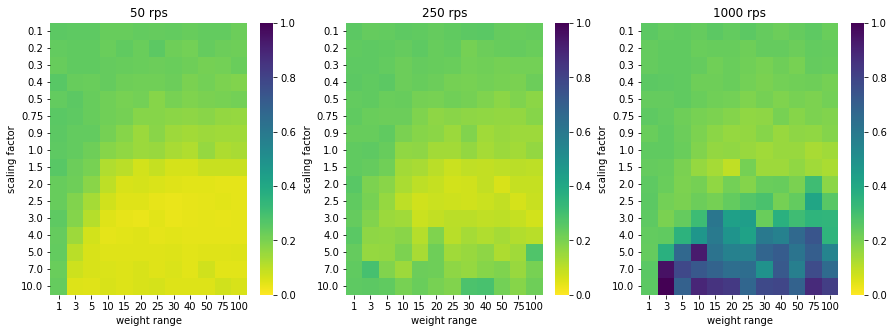
\includegraphics[width=14cm]{graphics/graphs/lb_hyper_scaling_vs_weight_range.png}
    \caption{Mean response time over different weight ranges and scaling factors}
    \label{fig:lb_hyper_weightrange_scaling}
\end{figure}

The results of this evaluation can be seen in Figure \ref{fig:lb_hyper_weightrange_scaling}.
Results show a clear trend towards higher weight ranges and scaling factors that are close to or slightly above 1, which would correspond to linear scaling.
We can also observe that higher request loads lead to worse performance on average, as one would expect, and also seem to shrink the set of configurations that provide good performance.

\subsubsection{Resetting Weights on Updates and Weight Update Intervals}
Our implementation of weighted round robin described earlier has a set of two weights for each upstream: the weight, and the current weight.
Once the weight of an upstream changes, we can choose to also reset the current weight or leave it as is.
Since intuitively there was no clear answer as to which choice is better, and the testing infrastructure around this was already in place, we chose to perform an experiment to measure the impact of this choice.
Apart from whether or not weights should be reset on updates, one also needs to decide at which interval weight updates should occur.
To evaluate this choice we performed these experiments using a variety of different update intervals.
Since we expected that resetting weights will have an outsized effect for scenarios with a low request rate, we performed experiments over a wider range of request loads than before, and also tested over different weight ranges.
Request load ranges from 2\gls{rps} to 1000\gls{rps}, weight update frequency from 5 seconds to 200 seconds, and maximum weight once again from 1 to 100.
Lastly, all experiments simulated a timeframe of 1000 seconds.

\begin{figure}
    \centering
    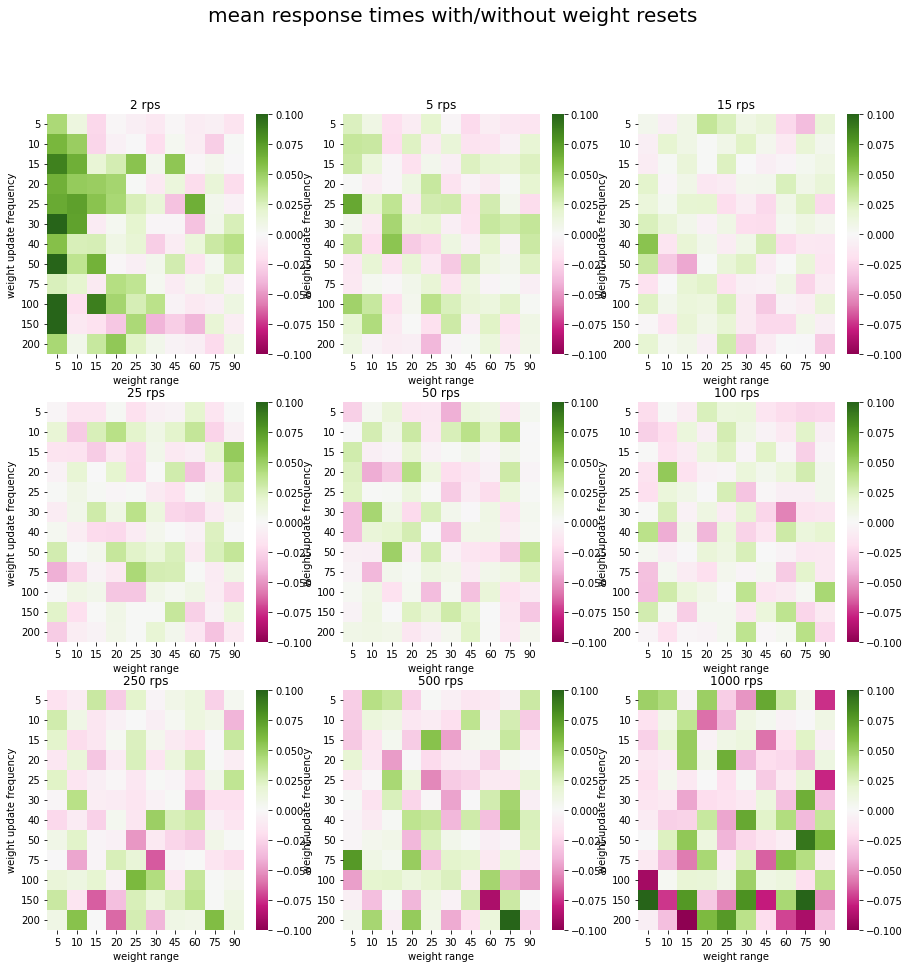
\includegraphics[width=14cm]{graphics/graphs/lb_hyper_weight_reset_delta.png}
    \caption{Difference between resetting and not resetting weights on update. Positive values indicate not resetting performs better, while negative values indicate the opposite.}
    \label{fig:lb_hyper_reset_delta}
\end{figure}

\begin{figure}
    \centering
    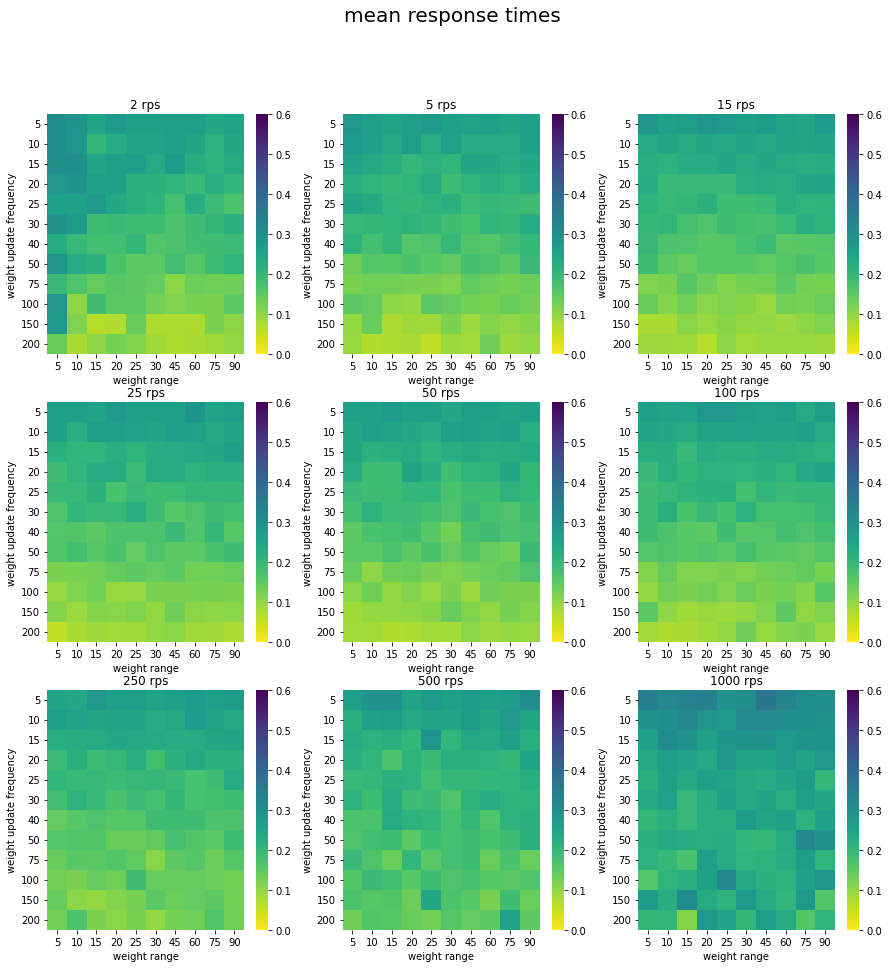
\includegraphics[width=14cm]{graphics/graphs/lb_hyper_mean_with_reset.png}
    \caption{Mean response times over different weight ranges and weight update times. Current weights are reset on update.}
    \label{fig:lb_hyper_reset_mean}
\end{figure}

\begin{figure}
    \centering
    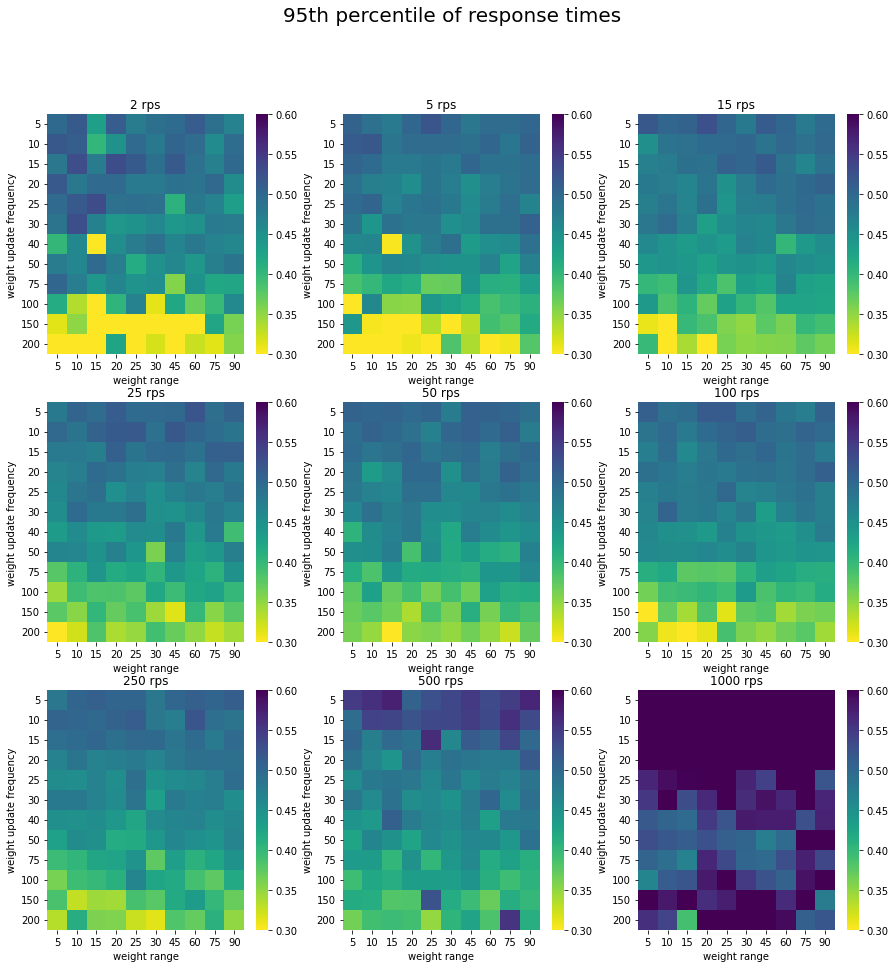
\includegraphics[width=14cm]{graphics/graphs/lb_hyper_95th_percentile_with_reset.png}
    \caption{95th percentile of response times over different weight ranges and update times. Current weights are reset on update.}
    \label{fig:lb_hyper_reset_q95}
\end{figure}

Figure \ref{fig:lb_hyper_reset_delta} shows the difference between the mean values of resetting or not resetting current weights.
In the results there is no clear indication resetting or not resetting is clearly superior.
There is a slight trend for not resetting performing better with low request rates, and resetting leading to better results in very high \gls{rps} scenarios.

Figure \ref{fig:lb_hyper_reset_mean} shows a trend towards longer intervals for weight updates performing better, irrespective of the weight range.
Figure \ref{fig:lb_hyper_reset_q95}, which shows the 95th percentile of the same data generally indicates the same tendency, although not for all request levels.
While at low request rates long update intervals perform better, they perform worse than shorter update intervals for high request rates.
Lastly we advise that care should be taken when comparing these visualizations, as the scale sometimes differs.
This is always indicated on the side of the visualization, and was necessary to better show relative differences within the same experiment run.


% Notes for discussion:
% QoS issue where one setting might be good under certain conditions, but bad under others e.g. 95th percentile type stuff
% extremes seem not to do so well for the most part
% behavious is to a large degree as expected: for low RPS super steep scaling works fine, but it becomes less good once capacity of the best nodes is reached
% No super clear point for or against weight resetting, once again depends on situation -> this points to a further investigation of the role of node discovery.
% to a degree weight resets perform a bit as expected in that low rps strongly prefer not resetting, and high rps preferring resets
% explanation why is quite intuitive, especially w.r.t. 

\section{Resource Usage and Load Balancer Scale}
\section{Load Balancer Resource Usage}
% 2 pages
\subsection{Performance Impact of Load Balancer Scale}
% 1 page
With this experiment we evaluate the effect different load balancer scales have on the system.
As we already described the quality and thus resulting end user performance of load balancer decisions only stabilizes after a while, since the load balancer first has to evaluate the available upstreams by sending requests to them.
Because of this, having larger numbers of load balancers present in the system might lead to delayed convergence, and thus suboptimal performance.
Having too few load balancers, on the other hand, might lead to lost performance through overly long routes.

To find out how different scales affect the overall system, we test the system performance with fixed percentages of nodes hosting load balancers.
We test a ranges between 5\% and 100\% of nodes hosting load balancers, which in our scenarios across three cities and 400 nodes means between 20 and 400 load balancer instances.
Scheduling load balancer replicas in these scenarios is still left to the Kubernetes scheduler, which means that the location of the node in the topology is not taken into account.

When testing ratios where less than 5\% of nodes hosted load balancers, we ran into frequent occurrences of the simulation not terminating within a feasible time window.
Upon investigation it turned out that if a load balancer was the only one in the city, or otherwise handled a lot of traffic, but happened to be placed onto a node with very limited bandwidth, the network simulation would take an exceedingly long time, because the bandwidth bottleneck resulted in each request only receiving a minuscule amount of bandwidth.
Requests that did go through took so long, that in real-life it would be considered a failed request by timeout.
We take this as an indication of the inherent problematic of current replica scheduling methods in edge computing, and that the usage of current techniques would simply require an outsized number of load balancers to mitigate the risk of such dysfunctional configurations.

The topologies tested are structurally similar to those of the initial evaluation.
Our two testing scenarios are three cities distributed across the United States, and three cities distributed across the globe.
The cities are identical to the ones from the initial evaluation, and feature identical network latencies between them.
The difference between these and the ones of the initial evaluation is that these feature a different internal topology, which is more closely related to edge intelligence\cite{rauschEdgeIntelligenceConvergence2019} and edge computing in general.
The cities in this evaluation have their compute capabilities, i.e. the cluster nodes, either in the city's local cloud data center, on a smart pole, or next to a cellular base station.
Clients are attached either to smart poles or directly to cellular base stations.
Cellular base stations themselves have a high-speed, high-bandwidth uplink to the wider network and feature a lower bandwidth and higher latency wireless connection to the clients.
These wireless properties depend on whether the cellular tower is LTE or 5G based, as both types are present in our scenario and their network properties are based on real world data\cite{braudMulticarrierMeasurementStudy2019}.
Not all cellular towers have directly attached compute capabilities.
In addition, one of the three cities does not feature a data center.

We simulate the cluster over the course of 2000 seconds, once with 25 \gls{rps}, once with 75\gls{rps}.

\begin{table}[]
\begin{tabular}{lrrrr}
\hline
                                                                             & \multicolumn{4}{c}{mean}                                                                                                                                                                                                                                              \\
\textbf{\begin{tabular}[c]{@{}l@{}}Nodes with\\ Load Balancers\end{tabular}} & \textbf{\begin{tabular}[c]{@{}r@{}}Global\\ 75rps\end{tabular}} & \textbf{\begin{tabular}[c]{@{}r@{}}Global\\ 25rps\end{tabular}} & \textbf{\begin{tabular}[c]{@{}r@{}}Nation\\ 75rps\end{tabular}} & \textbf{\begin{tabular}[c]{@{}r@{}}Nation\\ 25rps\end{tabular}} \\ \hline
\textbf{5\%}                                                                 & 210ms                                                           & 132ms                                                           & 220ms                                                           & 141ms                                                           \\
\textbf{10\%}                                                                & 149ms                                                           & 128ms                                                           & 158ms                                                           & 133ms                                                           \\
\textbf{20\%}                                                                & 134ms                                                           & 127ms                                                           & 147ms                                                           & 128ms                                                           \\
\textbf{30\%}                                                                & 132ms                                                           & 124ms                                                           & 141ms                                                           & 127ms                                                           \\
\textbf{40\%}                                                                & 130ms                                                           & 126ms                                                           & 135ms                                                           & 126ms                                                           \\
\textbf{50\%}                                                                & 128ms                                                           & 125ms                                                           & 134ms                                                           & 125ms                                                           \\
\textbf{60\%}                                                                & 129ms                                                           & 126ms                                                           & 133ms                                                           & 126ms                                                           \\
\textbf{70\%}                                                                & 129ms                                                           & 125ms                                                           & 128ms                                                           & 126ms                                                           \\
\textbf{80\%}                                                                & 128ms                                                           & 128ms                                                           & 131ms                                                           & 125ms                                                           \\
\textbf{90\%}                                                                & 129ms                                                           & 125ms                                                           & 129ms                                                           & 125ms                                                           \\
\textbf{100\%}                                                               & 127ms                                                           & 125ms                                                           & 129ms                                                           & 126ms                                                           \\ \hline
\end{tabular}
\caption{Mean \gls{trt} values of different load balancer scales, once they have converged to a stable value}
\label{tab:lb_scaling_converged_trt}
\end{table}

\begin{figure}
    \centering
    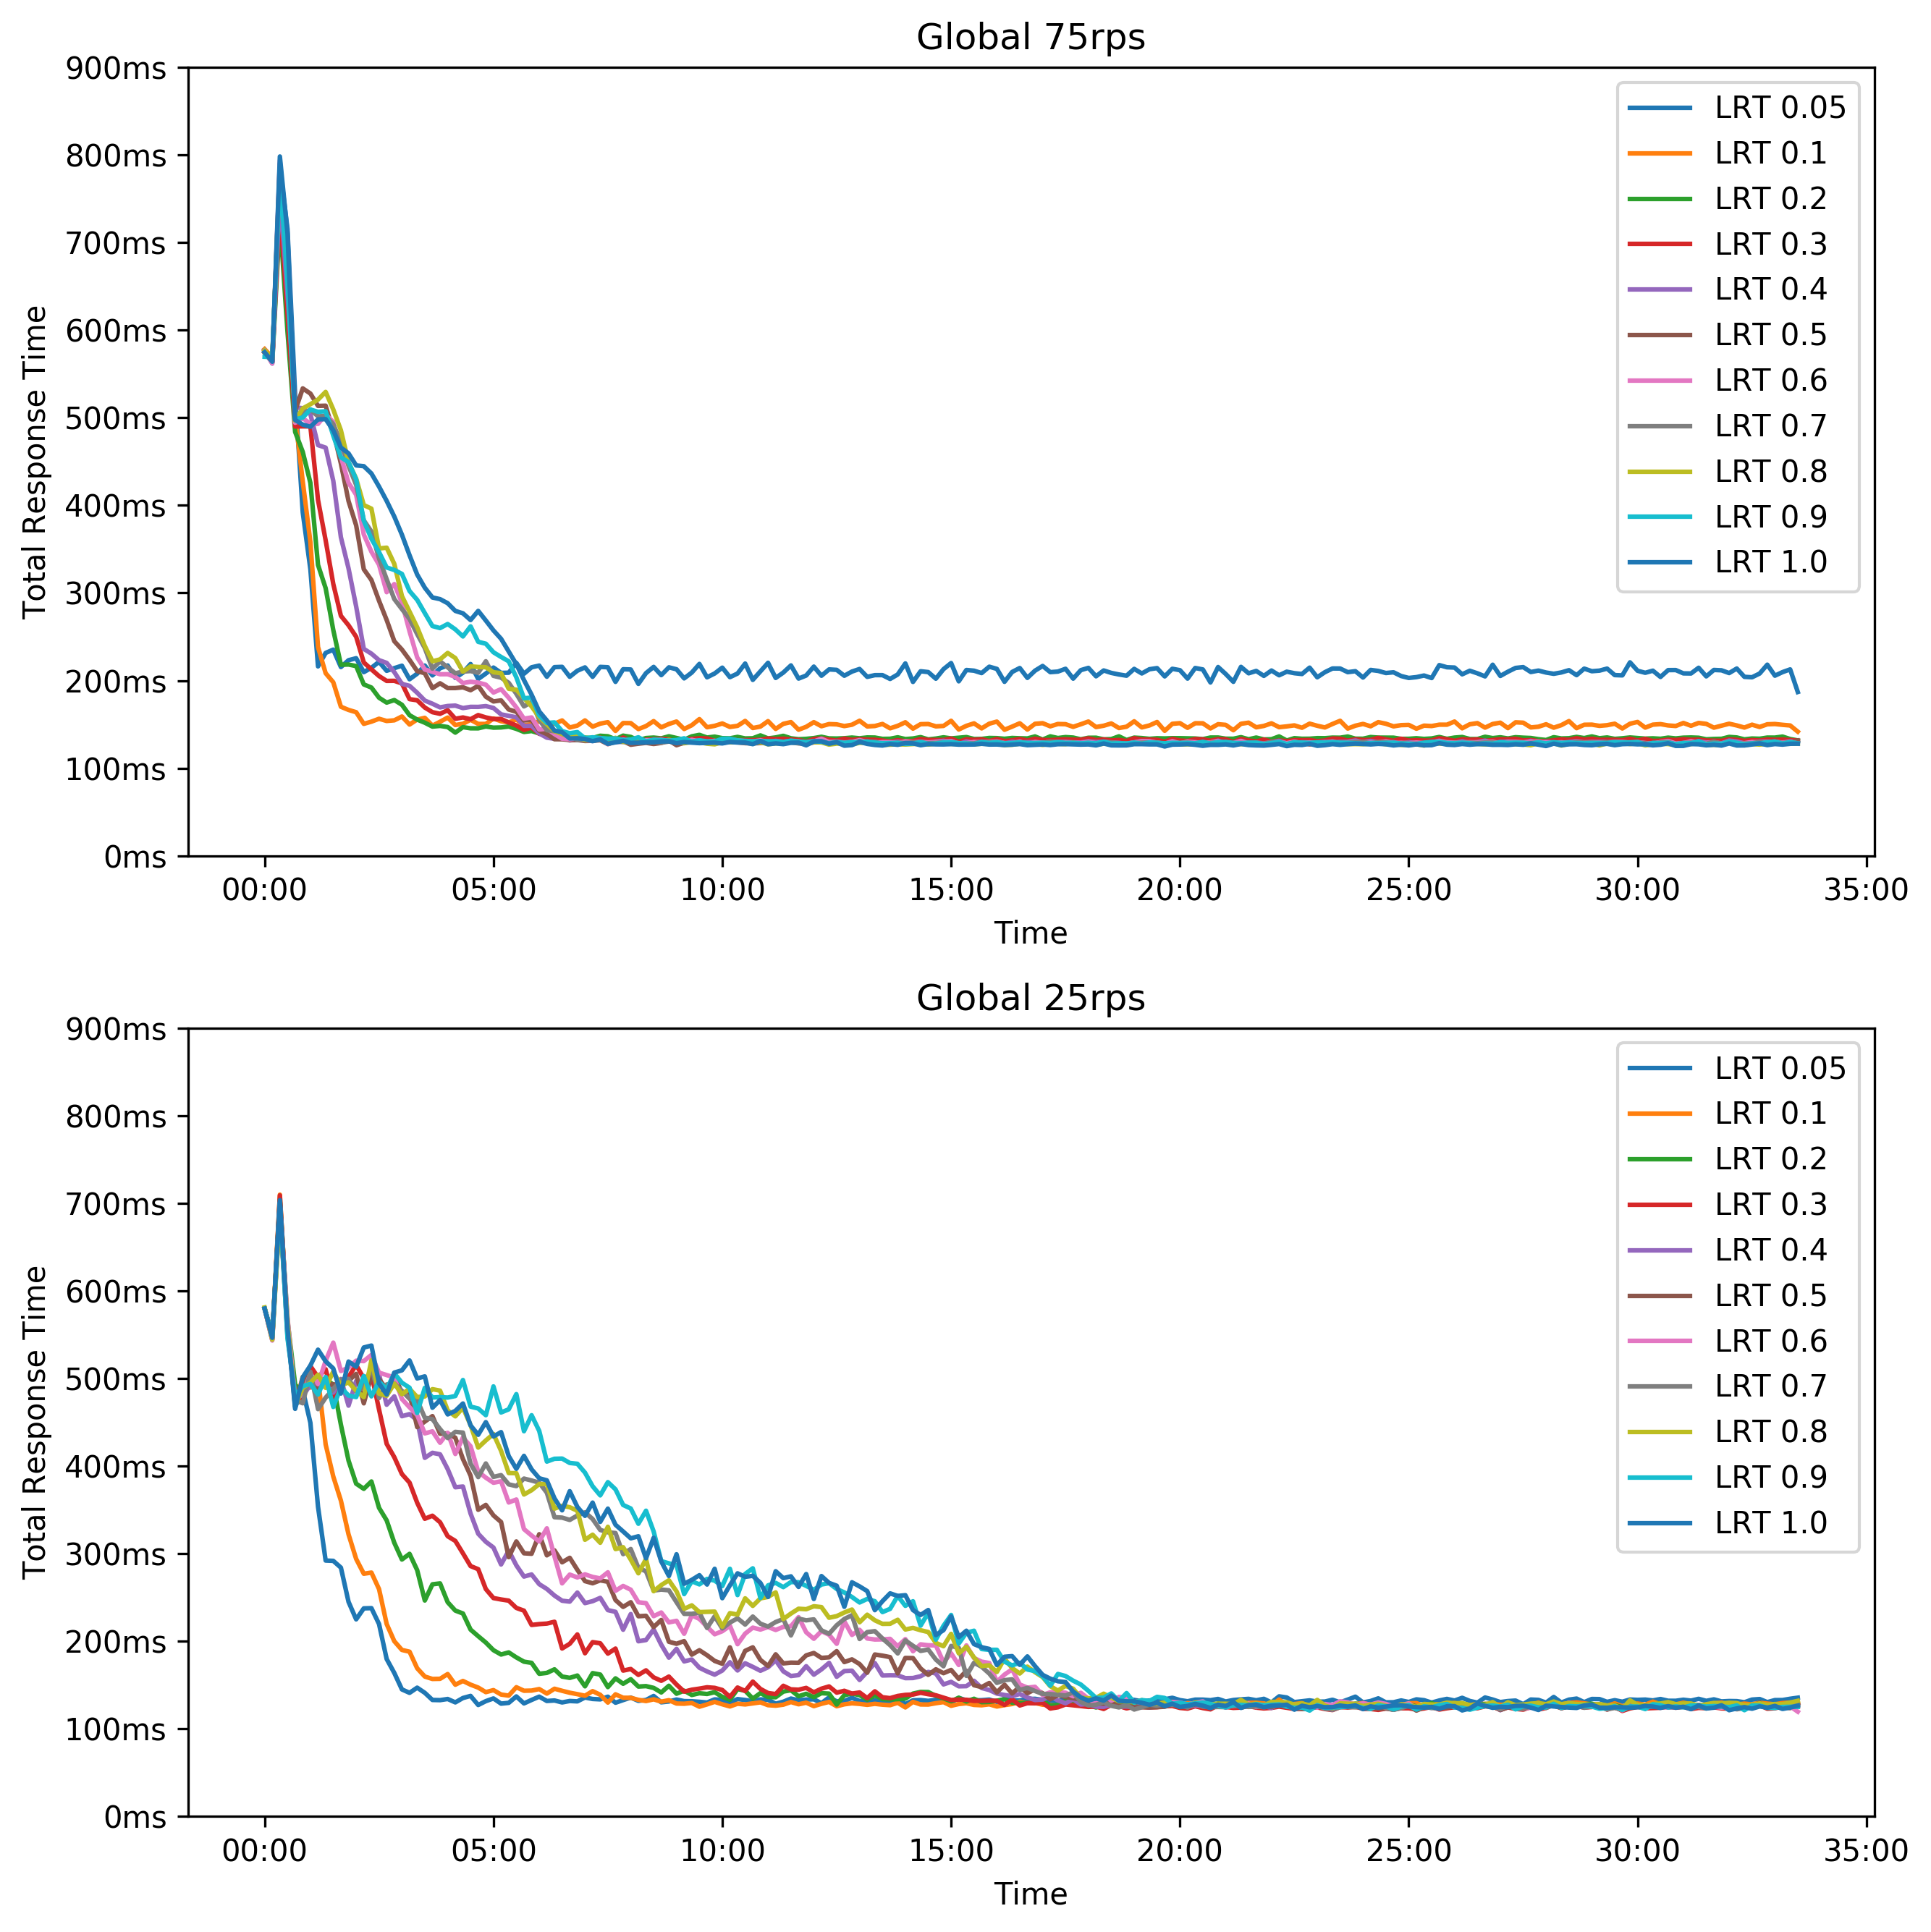
\includegraphics[width=\linewidth]{graphics/graphs/global_lb_scale_corrected.png}
    \caption{\glspl{trt} of different load balancer scales in the global scenario. For legibility a 10 second moving average is applied.}
    \label{fig:lb_scale_global}
\end{figure}

\begin{figure}
    \centering
    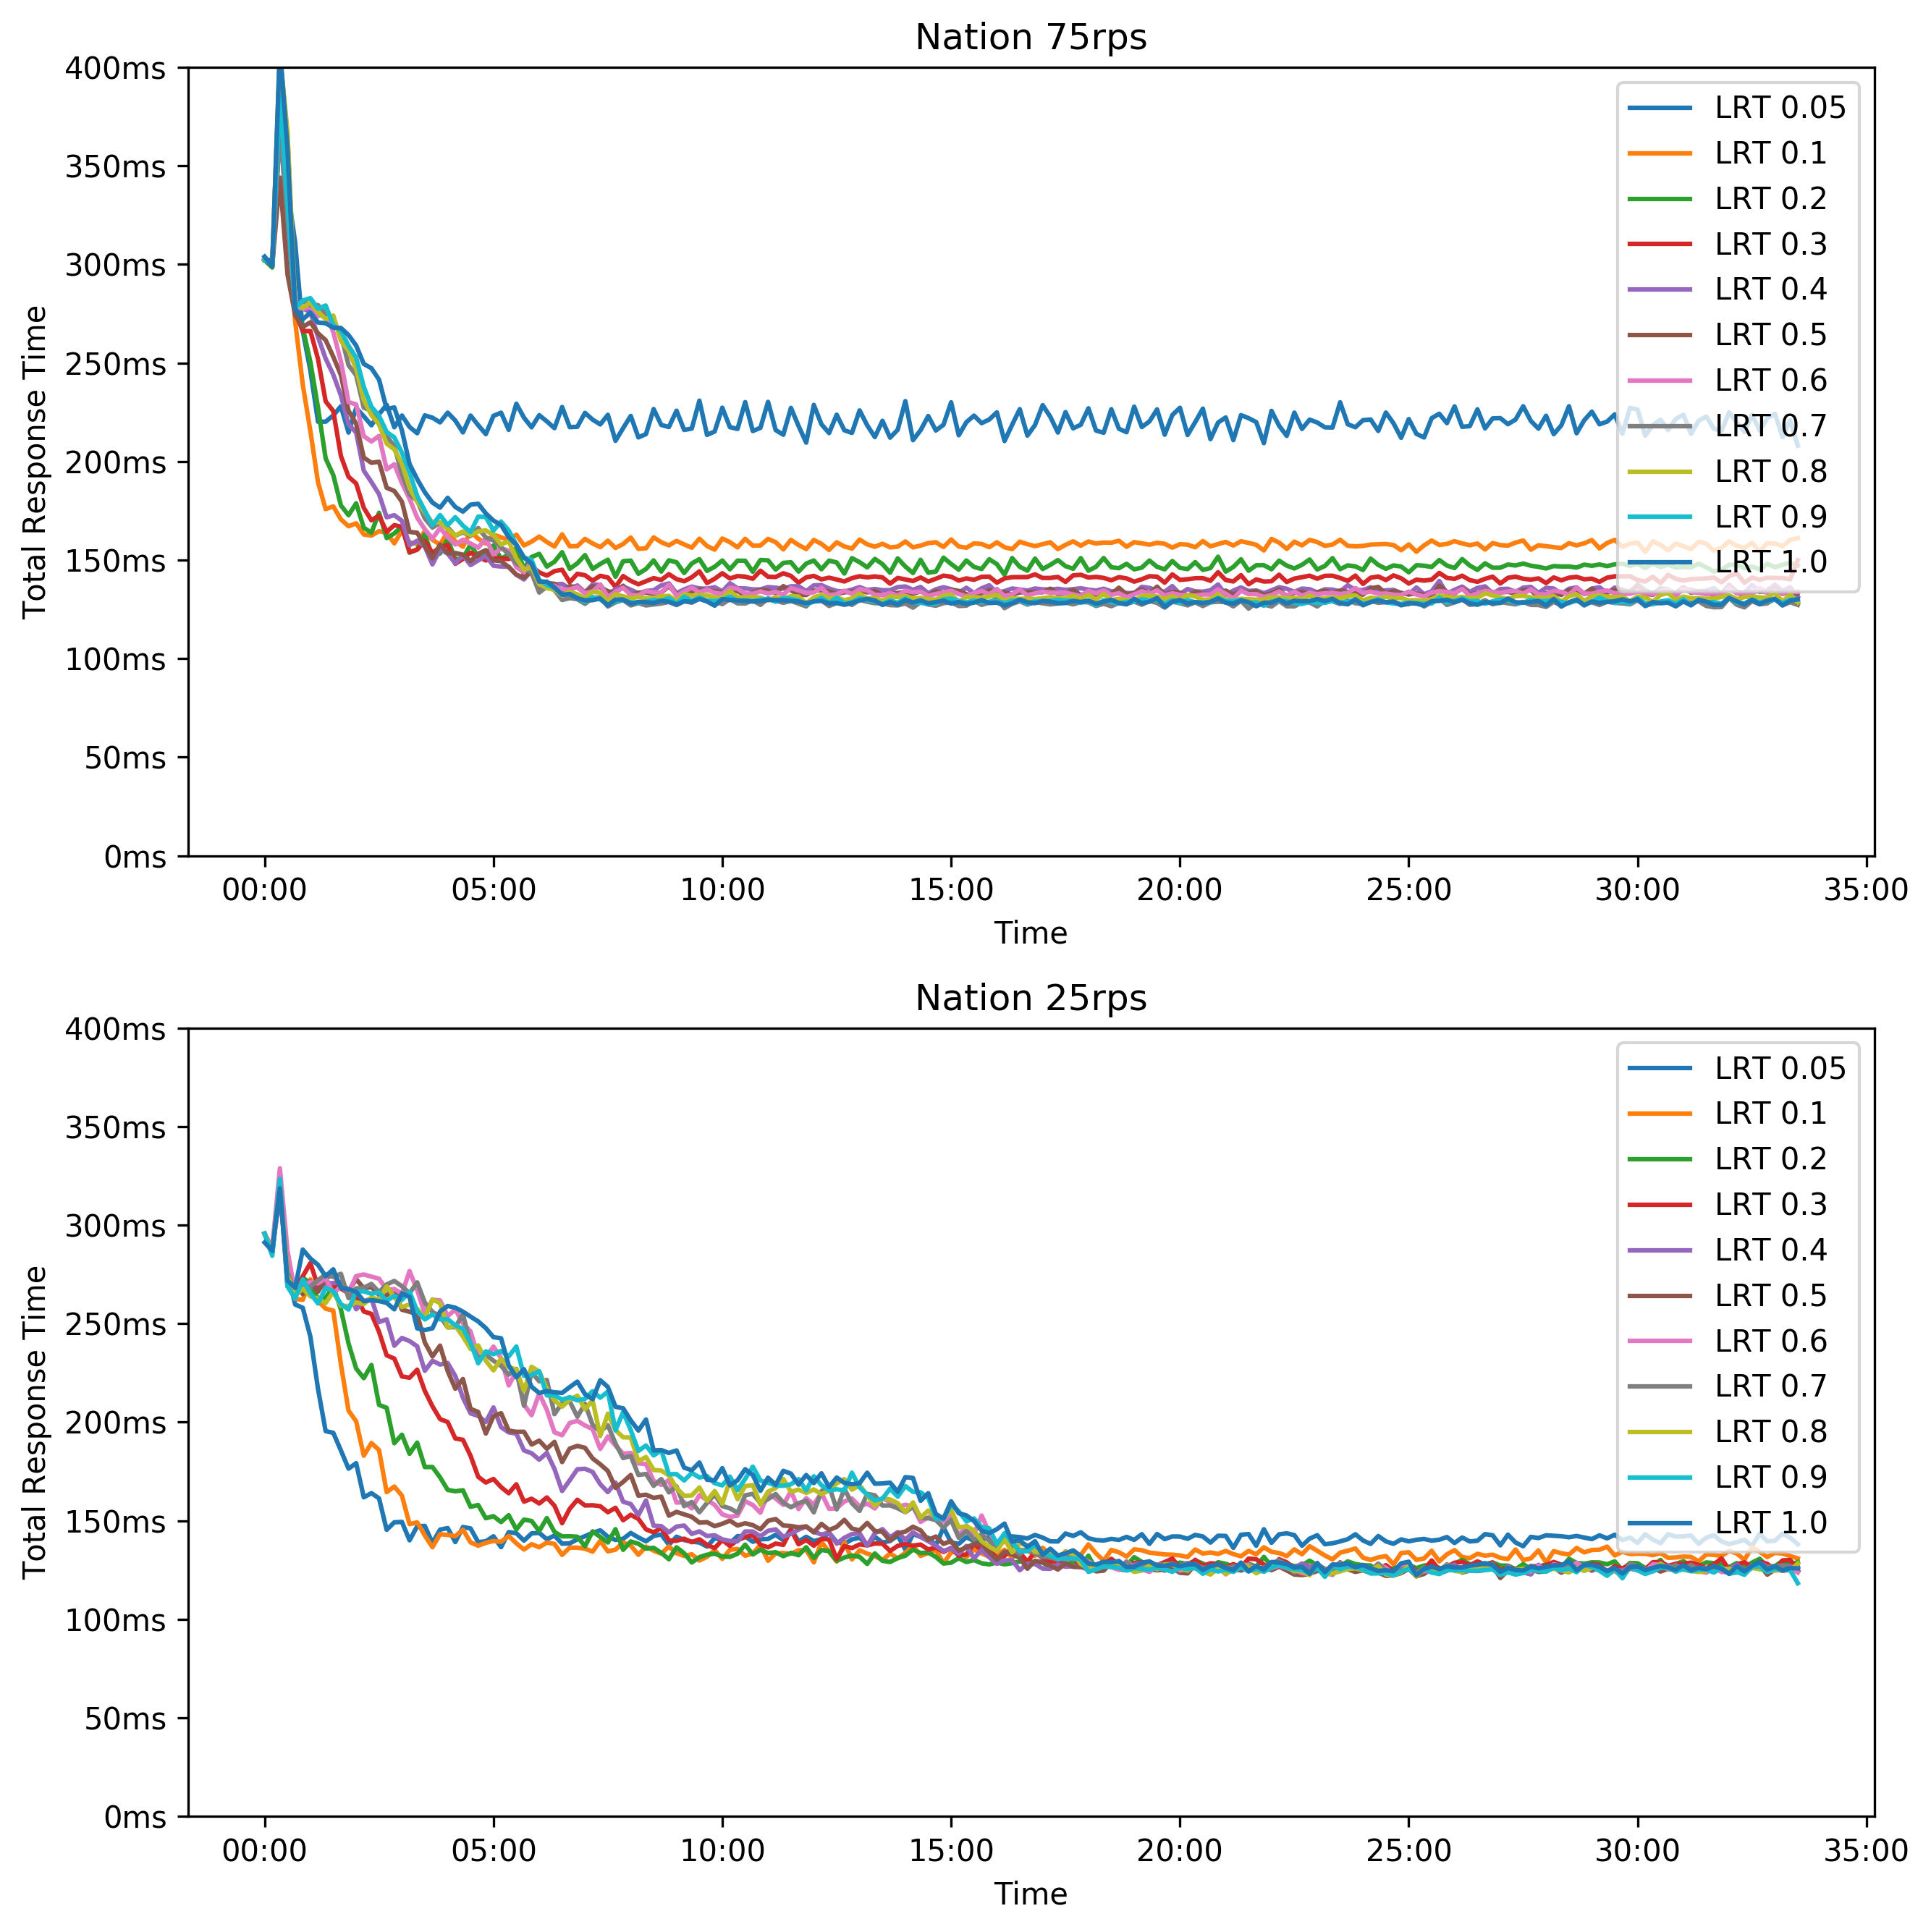
\includegraphics[width=\linewidth]{graphics/graphs/nation_lb_scale_corrected.png}
    \caption{\glspl{trt} of different load balancer scales in the nation scenario. For legibility a 10 second moving average is applied.}
    \label{fig:lb_scale_nation}
\end{figure}

Our results show consistent patterns across both topologies, but differ across the request rate.
While in scenarios with a request rate of 75 \gls{rps} higher numbers of load balancers lead to improved mean response time, in scenarios with 25 \gls{rps} lower numbers perform better.
Figures \ref{fig:lb_scale_global} and \ref{fig:lb_scale_nation} show explanations for this behaviour.
With lower numbers of load balancers the request rate per load balancer is higher, and thus leads to faster convergence towards a stable and efficient response time.

Table \ref{tab:lb_scaling_converged_trt} shows the mean response times of different load balancer scales once response times have stabilized.
Once only stabilized values are considered higher numbers of load balancers lead to improved performance.
Figures \ref{fig:lb_scale_global} and \ref{fig:lb_scale_nation} show this too, where lower numbers of load balancers stabilize earlier, but at higher \gls{trt} values.
From Table \ref{tab:lb_scaling_converged_trt} we also see that between the different load balancer scales, differences in response time become negligible at a certain point, with load balancers on 50\% of nodes converging to almost the same mean response time as having load balancers on 100\% of nodes.

Lastly, we observe that the absolute difference between the time when the system performs best, and when the system performs worst is dependent on topology make up.
The globally distributed scenario has the potential to perform worse, as there is a greater likelihood of poor request routing decisions resulting in longer network distances.

The results of this experiment are closely related to the pressure threshold for load balancer scaling in our approach.
Subsequent evaluations explore how different thresholds result in different load balancer scales and thus different system performance with our osmotic scaling.



\section{Osmotic Scaling and Scheduling}
\subsection{Performance of Osmotic Scaling and Load Balancing}
% 2 pages
With this experiment we want to provide baseline performance data for the osmotic scaling and scheduling method we propose. The goal is to show how our proposed solution operates without fine-tuning of parameters, or any other conditions. The experiment should also show how the osmotic scaling and scheduling of load balancers affects other parts of the serverless system, most notably the scaling decisions of regular functions.
\subsubsection{Setup}
Our experiment setup for these evaluations is once again based on the serverless edge computing simulator we also used for the initial evaluations. To stay consistent we used the same network topologies from the previous experiment that investigated the impact of load balancer scale on the system, meaning we assume clients to typically be connected via a mobile network, and compute resources to be distributed on the edge. The three topologies we tested are once again one scenario with a single city, one with three cities on the same continent, and one with three cities distributed across the globe. The cities chosen, along with the network latencies between them are the same as in the initial evaluation namely Chicago, New York, and Seattle for the nation-distibuted and New York, London, and Sydney for the globally-distributed experiment. The network latencies between them can be seen in tables \ref{tab:initial_nation_pings} and \ref{tab:initial_global_pings} respectively.

To stay consistent with the other experiments, and partially due to performance limitations, we once again tested each topology scenario with 25\gls{rps}, 50\gls{rps}, and 75\gls{rps}. As for the osmotic scaling and scheduling component, we set the pressure threshold for scaling up to 0.025 and the downscaling threshold to 0.03, which can roughly be read as the system requiring an expected \gls{trt} improvement of 2.5\% and 3\% to add or remove a load balancer instance on a given node. Bear in mind that this idea of required estimated performance improvement is a mental model to get a more intuitive understanding for the parameters, and is not equivalent to the actual implementation.

The last way in which the experiment setup differs from the previous experiments is that there is a function scheduling component active. While the other experiments purposefully set a fixed scale for each of the serverless functions in the system to avoid it as a confounding variable, these experiments use a dynamic function scaler to show how this type of load balancer scaling and scheduling affects the overall system.
In concrete terms, we set the simulator up to use a set rate of average requests per function replica.
The reasoning behind this choice is that OpenFaaS uses the same methodology as a default configuration, which we use as a stand-in example of serverless computing frameworks in general.
For the osmotic scaling and scheduling parameters we used 0.03 as a scale-up threshold and 0.05 as a scale-down threshold.

\subsubsection{Results}

\begin{table}[]
\begin{tabular}{lrrrrrr}
\hline
\textbf{Experiment}  & \textbf{\begin{tabular}[c]{@{}r@{}}LB\\ replicas\end{tabular}} & \textbf{\begin{tabular}[c]{@{}r@{}}Converged\\ Total \\ Function\\ Replicas\end{tabular}} & \textbf{\begin{tabular}[c]{@{}r@{}}Cross-City\\ Request\\ Share\end{tabular}} & \textbf{\begin{tabular}[c]{@{}r@{}}Mean\\ TRT\end{tabular}} & \textbf{\begin{tabular}[c]{@{}r@{}}Median\\ TRT\end{tabular}} & \textbf{\begin{tabular}[c]{@{}r@{}}Q90\\ TRT\end{tabular}} \\ \hline
25rps City LRT       & 6                                                              & 88                                                                                        & 0.0\%                                                                         & 121ms                                                       & 121ms                                                         & 157ms                                                      \\
25rps City Osmotic   & 24                                                             & 89                                                                                        & 0.0\%                                                                         & 117ms                                                       & 119ms                                                         & 149ms                                                      \\
25rps City RR        & 6                                                              & 90                                                                                        & 0.0\%                                                                         & 168ms                                                       & 136ms                                                         & 275ms                                                      \\ \hline
25rps Nation LRT     & 14                                                             & 89                                                                                        & 17.0\%                                                                        & 154ms                                                       & 131ms                                                         & 254ms                                                      \\
25rps Nation Osmotic & 3                                                              & 88                                                                                        & 32.5\%                                                                        & 224ms                                                       & 208ms                                                         & 386ms                                                      \\
25rps Nation RR      & 14                                                             & 90                                                                                        & 65.4\%                                                                        & 274ms                                                       & 266ms                                                         & 432ms                                                      \\ \hline
25rps Global LRT     & 14                                                             & 94                                                                                        & 0.4\%                                                                         & 142ms                                                       & 126ms                                                         & 210ms                                                      \\
25rps Global Osmotic & 5                                                              & 90                                                                                        & 1.7\%                                                                         & 152ms                                                       & 128ms                                                         & 224ms                                                      \\
25rps Global RR      & 14                                                             & 99                                                                                        & 65.4\%                                                                        & 501ms                                                       & 410ms                                                         & 937ms                                                      \\ \hline
50rps City LRT       & 6                                                              & 249                                                                                       & 0.0\%                                                                         & 127ms                                                       & 124ms                                                         & 177ms                                                      \\
50rps City Osmotic   & 13                                                             & 249                                                                                       & 0.0\%                                                                         & 123ms                                                       & 123ms                                                         & 164ms                                                      \\
50rps City RR        & 6                                                              & 249                                                                                       & 0.0\%                                                                         & 162ms                                                       & 141ms                                                         & 248ms                                                      \\ \hline
50rps Nation LRT     & 14                                                             & 179                                                                                       & 17.7\%                                                                        & 153ms                                                       & 129ms                                                         & 270ms                                                      \\
50rps Nation Osmotic & 5                                                              & 177                                                                                       & 24.3\%                                                                        & 165ms                                                       & 135ms                                                         & 283ms                                                      \\
50rps Nation RR      & 14                                                             & 181                                                                                       & 65.0\%                                                                        & 271ms                                                       & 264ms                                                         & 430ms                                                      \\ \hline
50rps Global LRT     & 14                                                             & 190                                                                                       & 1.2\%                                                                         & 147ms                                                       & 128ms                                                         & 213ms                                                      \\
50rps Global Osmotic & 4                                                              & 181                                                                                       & 3.8\%                                                                         & 159ms                                                       & 128ms                                                         & 238ms                                                      \\
50rps Global RR      & 14                                                             & 197                                                                                       & 65.1\%                                                                        & 494ms                                                       & 410ms                                                         & 922ms                                                      \\ \hline
75rps City LRT       & 6                                                              & 249                                                                                       & 0.0\%                                                                         & 127ms                                                       & 123ms                                                         & 175ms                                                      \\
75rps City Osmotic   & 14                                                             & 249                                                                                       & 0.0\%                                                                         & 122ms                                                       & 122ms                                                         & 162ms                                                      \\
75rps City RR        & 6                                                              & 249                                                                                       & 0.0\%                                                                         & 168ms                                                       & 140ms                                                         & 275ms                                                      \\ \hline
75rps Nation LRT     & 14                                                             & 269                                                                                       & 14.9\%                                                                        & 150ms                                                       & 129ms                                                         & 260ms                                                      \\
75rps Nation Osmotic & 5                                                              & 264                                                                                       & 24.1\%                                                                        & 169ms                                                       & 138ms                                                         & 287ms                                                      \\
75rps Nation RR      & 14                                                             & 269                                                                                       & 65.2\%                                                                        & 273ms                                                       & 269ms                                                         & 433ms                                                      \\ \hline
75rps Global LRT     & 14                                                             & 278                                                                                       & 0.1\%                                                                         & 141ms                                                       & 128ms                                                         & 214ms                                                      \\
75rps Global Osmotic & 5                                                              & 268                                                                                       & 1.9\%                                                                         & 152ms                                                       & 129ms                                                         & 223ms                                                      \\
75rps Global RR      & 14                                                             & 285                                                                                       & 65.2\%                                                                        & 497ms                                                       & 406ms                                                         & 928ms                                                      \\ \hline
\end{tabular}
\caption{Osmotic baseline evaluation results}
\label{tab:osmotic_base}
\end{table}

\begin{figure}
    \centering
    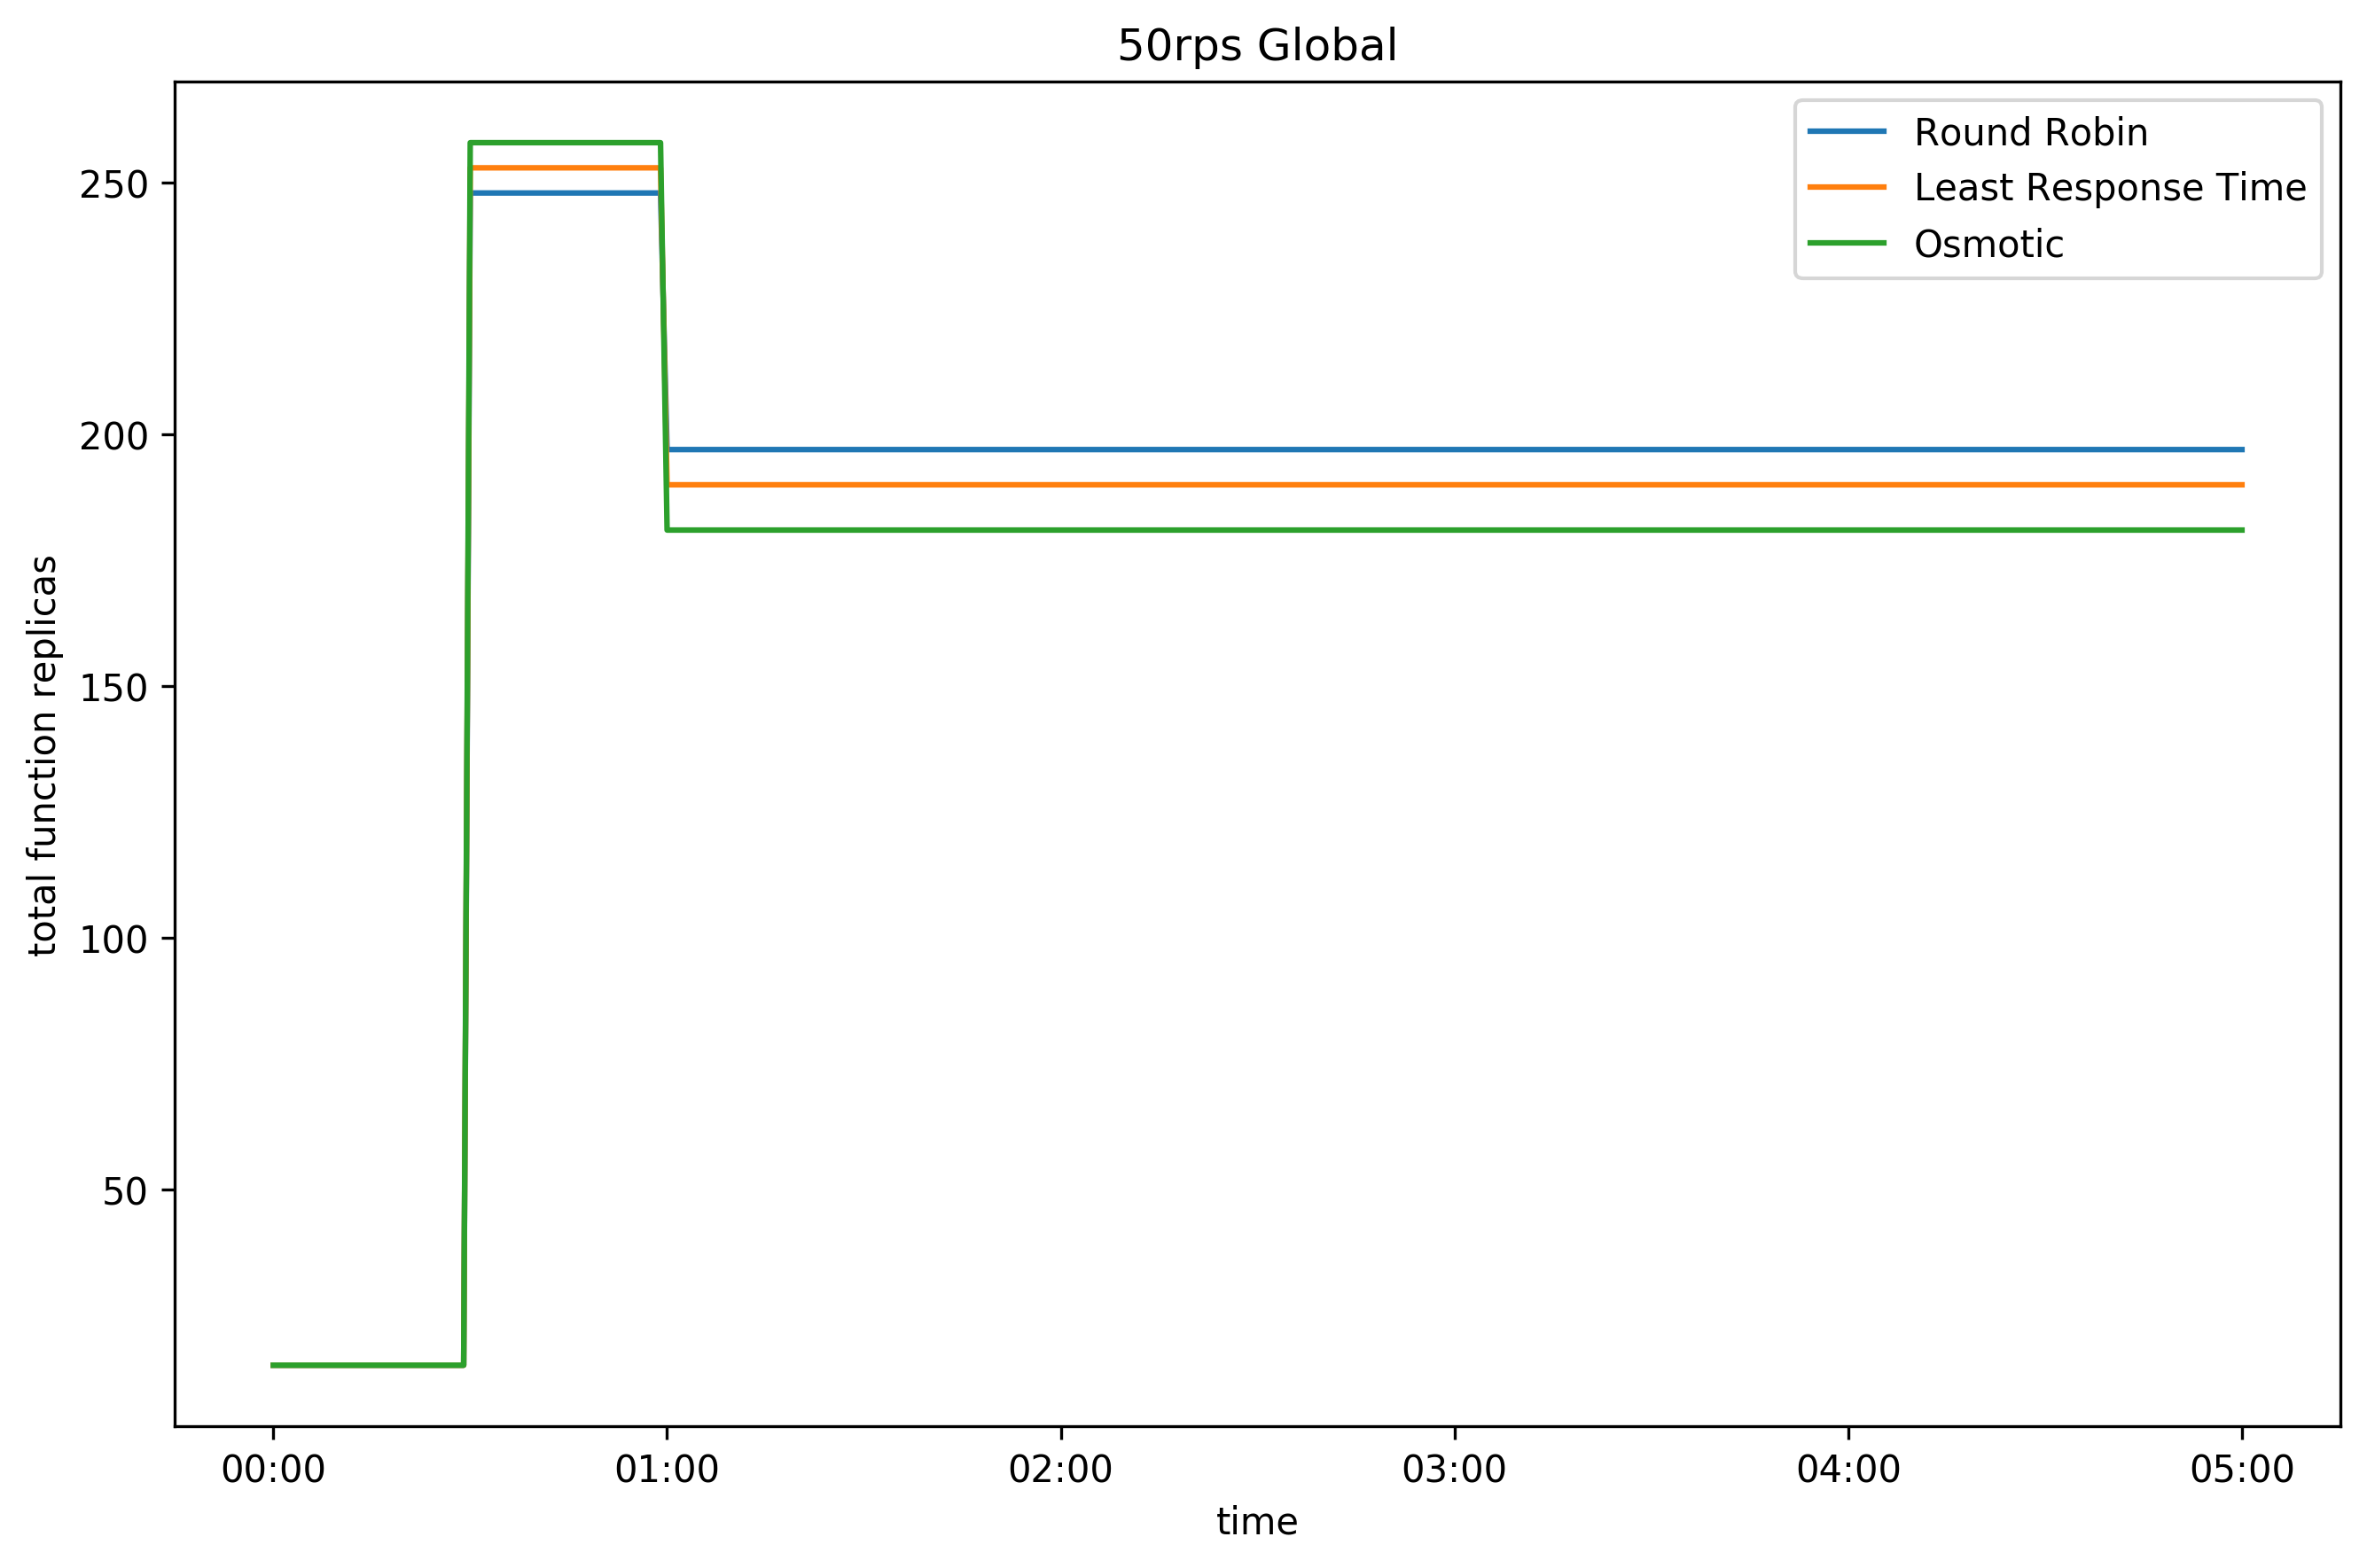
\includegraphics[width=12cm]{graphics/graphs/osmotic_base_function_scale_by_lb.png}
    \caption{Total scale of all functions for each load balancer scaling/schedulilng method}
    \label{fig:osmotic_fx_scale_by_scaling}
\end{figure}

Table \ref{tab:osmotic_base} shows the results of the experiment.
In terms of mean \gls{trt} performance the results of our proposed osmotic scaling and scheduling method are similar to those of the fixed scaling LRT reference setup, albeit between 1\% and 45\% worse with most scenarios only between 2\% and 8\% worse.
Differences between least response time static, and osmotic scaling are less pronounced in the median and 90th percentile \glspl{trt} as can also be seen in Table \ref{tab:osmotic_base}.
The statically scaled round robin load balancing is, as one would expect, significantly worse.
It does, however, give a good impression of the performance improvements possible based on our approach in a more complex and realistic deployment scenario than the initial evaluation.

We can also observe that in the city scenario the osmotic scaling and scheduling ends up deploying the more load balancer instances than the static scaling, but that for the nation- and globally-distributed network topology scenarios this patterns is reversed. There the osmotic scaler deploys only about a third of the replicas of the static scaling.

A similar pattern can be seen with regard to function scaling.
The osmotic scaling leads to between 1\% and 6\% fewer function replicas being deployed. Figure \ref{fig:osmotic_fx_scale_by_scaling} shows how the timing and frequency of scaling decisions are not different between the scaling methods, but osmotic scaling results in slightly fewer function replicas. 
\subsection{Optimization Aggressiveness with Osmotic Scaling}
We already learned from the experiment about load balancer scale that there is a tendency for a higher scale of load balancers to ultimately result in better performance.
With this experiment we want to test the interplay of this phenomenon with the osmotic load balancing and scaling we propose. With our osmotic approach we can set the scale-up threshold to more or less arbitrary values to influence how quickly or slowly the system scales up the number of load balancers, and how many load balancers will thus ultimately end up being deployed.

\subsubsection{Setup}
To test the performance we simulate a number of different configuration scenarios. For the rest of the system environment we choose to reuse the globally distributed topology from previous experiments with a request rate of 75\gls{rps} being simulated over the course of 2000 seconds.

For the parameters of the osmotic scaling and scheduling we run experiments for a range of scale-up thresholds ranging from 0.02 to 0.1.
The scale down threshold is always set to 0.2, which is relatively high, because we explicitly want to test how the scale-up threshold can be used to determine how many load balancers the system will deploy to optimize response times.

\subsubsection{Results}

\begin{table}[]
\begin{tabular}{lrrrrr}
\hline
\textbf{\begin{tabular}[c]{@{}l@{}}Upscaling\\ Pressure\\ Threshold\end{tabular}} & \textbf{\begin{tabular}[c]{@{}r@{}}LB\\ Replicas\end{tabular}} & \textbf{\begin{tabular}[c]{@{}r@{}}Mean\\ TRT\end{tabular}} & \textbf{\begin{tabular}[c]{@{}r@{}}Mean\\ FET\end{tabular}} & \textbf{\begin{tabular}[c]{@{}r@{}}Mean\\ LB\_FX\end{tabular}} & \textbf{\begin{tabular}[c]{@{}r@{}}Mean\\ CL\_LB\end{tabular}} \\ \hline
0.1                                                                               & 4                                                              & 155.8ms                                                     & 29.1ms                                                      & 33.5ms                                                         & 92.7ms                                                         \\
0.09                                                                              & 4                                                              & 152.5ms                                                     & 29.7ms                                                      & 30.1ms                                                         & 92.2ms                                                         \\
0.08                                                                              & 6                                                              & 152.1ms                                                     & 29.5ms                                                      & 30.0ms                                                         & 92.2ms                                                         \\
0.07                                                                              & 5                                                              & 152.5ms                                                     & 29.3ms                                                      & 30.4ms                                                         & 92.4ms                                                         \\
0.06                                                                              & 5                                                              & 148.5ms                                                     & 29.6ms                                                      & 26.6ms                                                         & 91.6ms                                                         \\
0.05                                                                              & 5                                                              & 147.5ms                                                     & 29.9ms                                                      & 25.3ms                                                         & 91.3ms                                                         \\
0.04                                                                              & 5                                                              & 148.5ms                                                     & 29.8ms                                                      & 26.5ms                                                         & 91.5ms                                                         \\
0.03                                                                              & 7                                                              & 136.8ms                                                     & 26.4ms                                                      & 19.6ms                                                         & 91.2ms                                                         \\
0.02                                                                              & 20                                                             & 139.0ms                                                     & 24.8ms                                                      & 25.3ms                                                         & 90.2ms                                                         \\ \hline
\end{tabular}
\caption{Response time performance metrics for different upscaling pressure thresholds}
\label{tab:osmotic_scaling_aggressiveness}
\end{table}





\begin{figure}
    \centering
    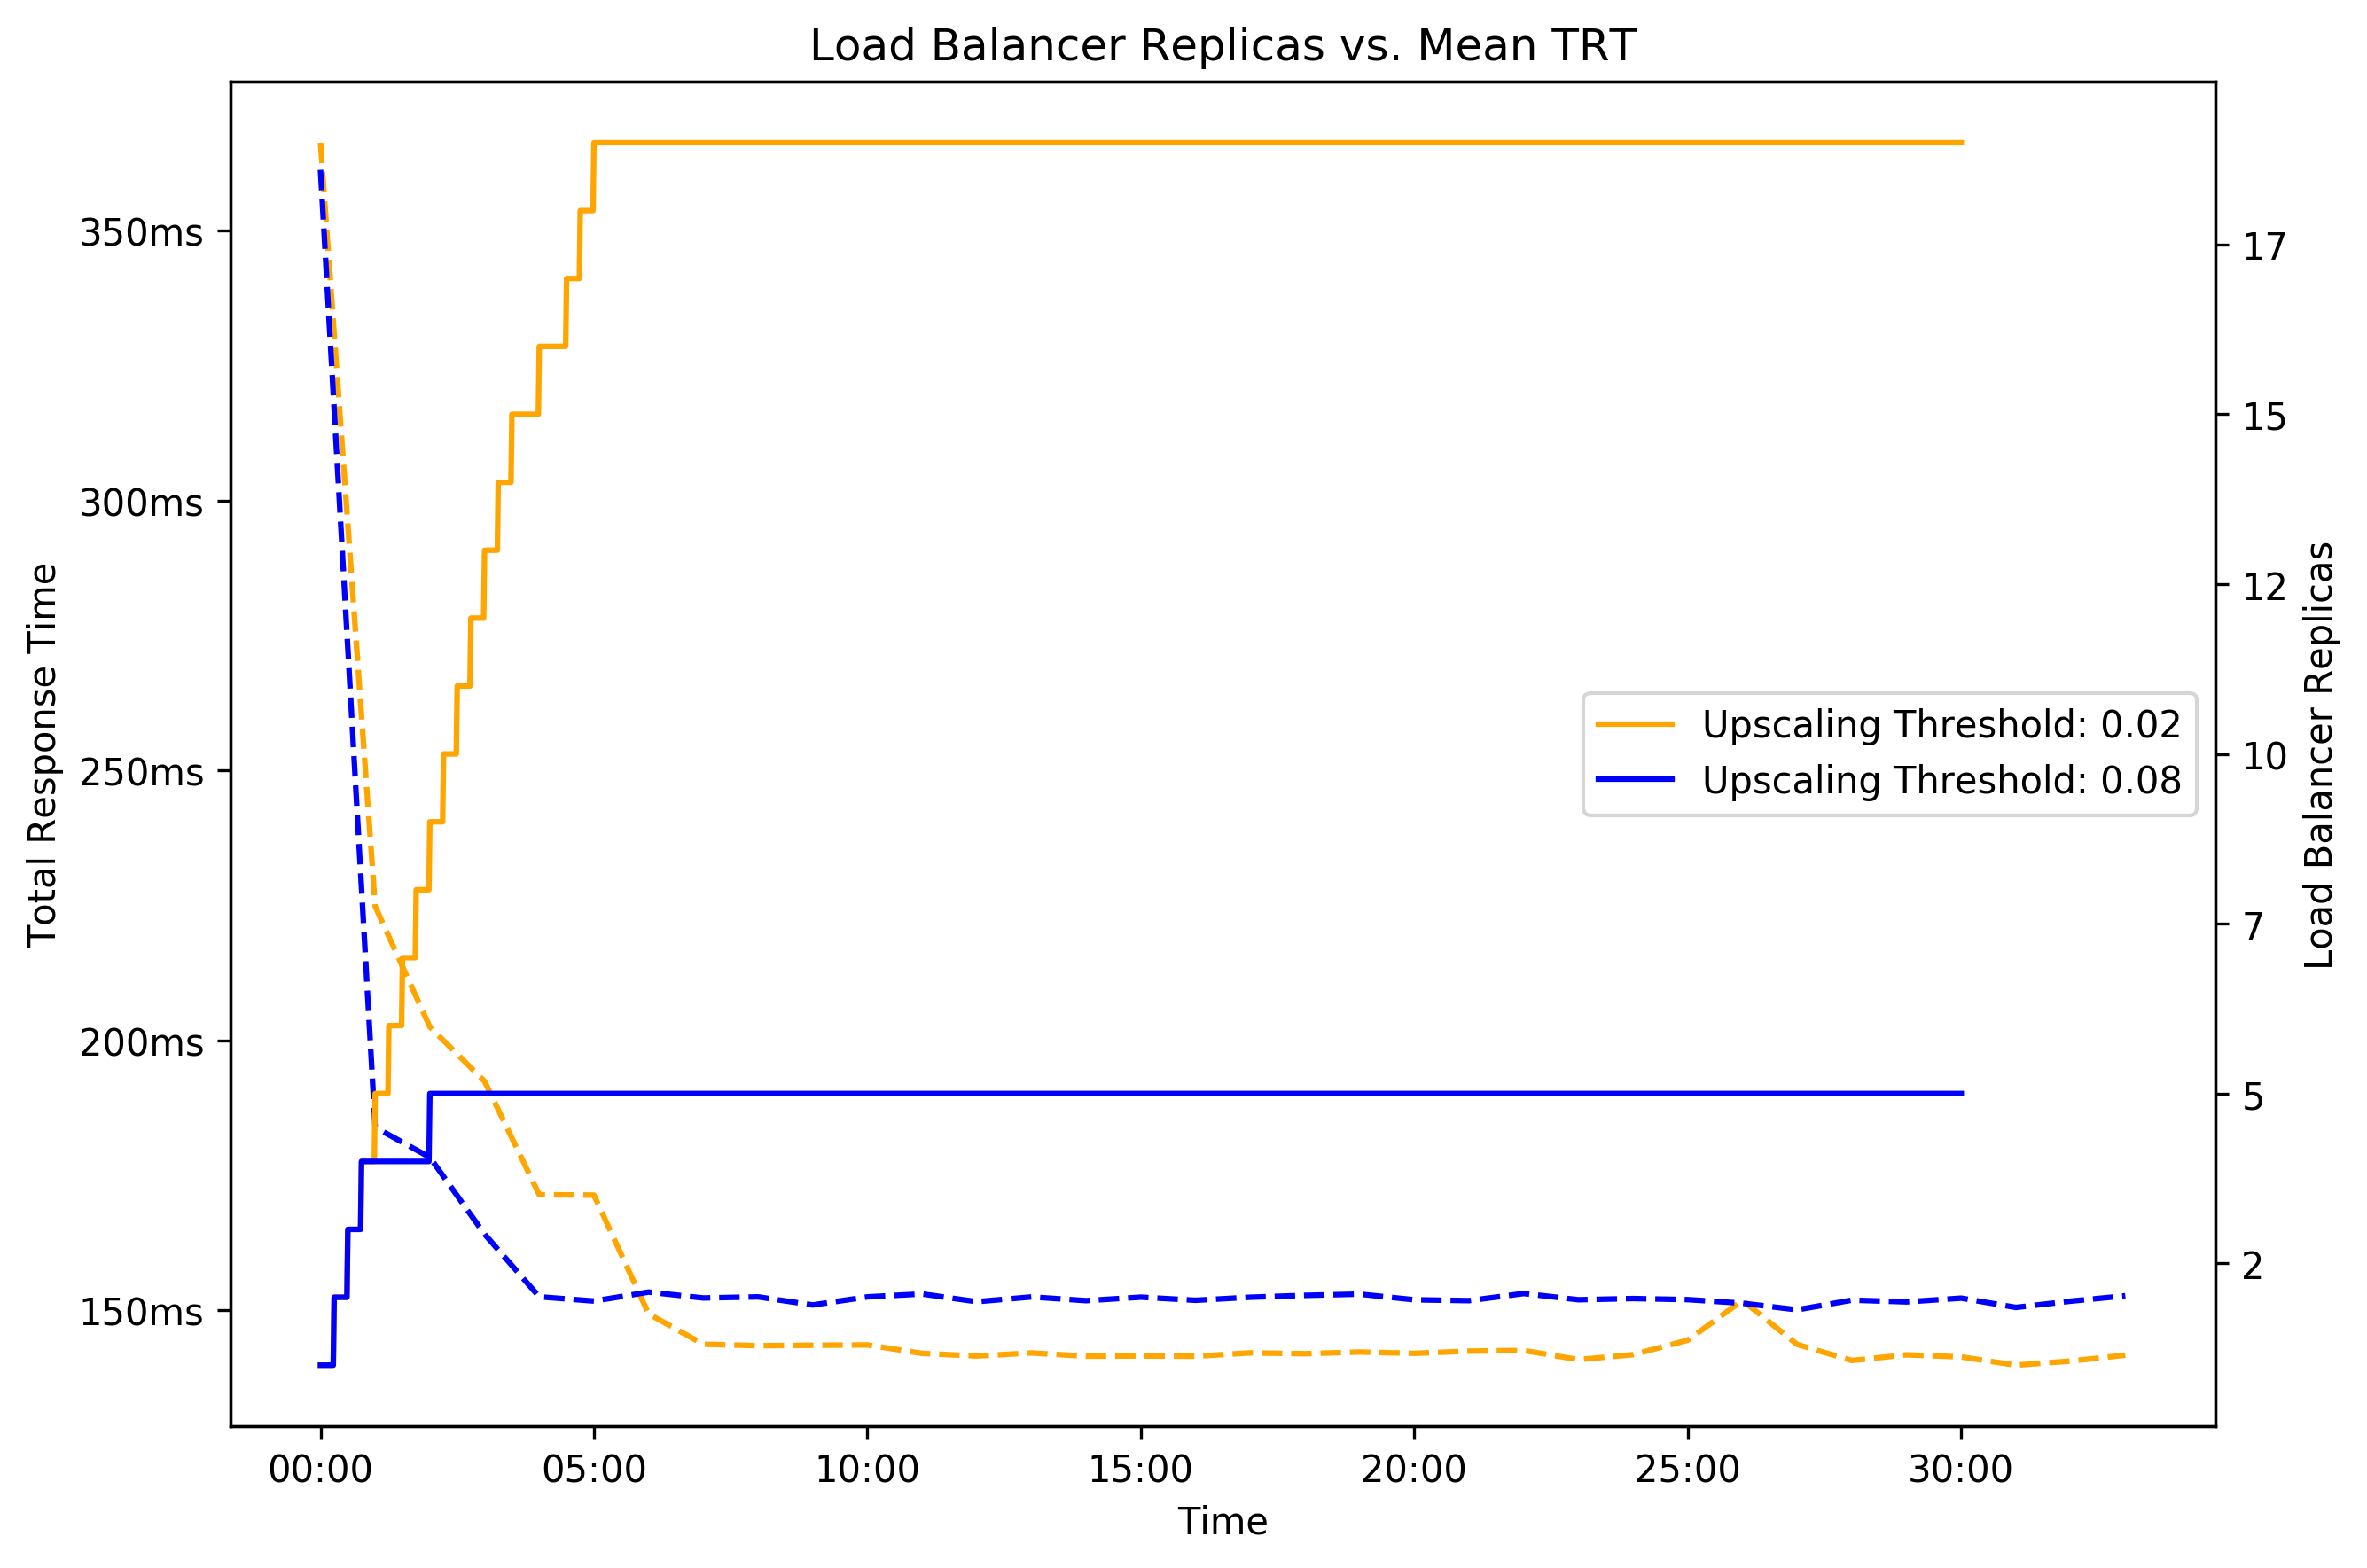
\includegraphics[width=12cm]{graphics/graphs/osmotic_optim_thres_vs_trt_corrected.png}
    \caption{\gls{trt} compared to current load balancer scale for two different osmotic scaling parametrizations}
    \label{fig:osmotic_trt_vs_replica_scale}
\end{figure}

The results show two clear trends.
First that will lower upscaling pressure thresholds more load balancer replicas are being deployed by the osmotic scaling component, and second that the mean response time improves with higher number of load balancer replicas.
As Table \ref{tab:osmotic_scaling_aggressiveness} shows, there is a diminishing return with higher numbers of load balancers, at least in the topology scenario tested.
The results also show that while higher numbers of load balancers provide better performance once the load balancers have gathered enough information about available replicas, this process is faster the fewer load balancers there are, thus giving better performance early on.
The behaviour can be observed easily in the graph in Figure \ref{fig:osmotic_trt_vs_replica_scale}.
\subsection{Osmotic Scheduling in Dynamic Systems}
% 3+ pages (complicated setup, no?)
In this last experiment we test the behaviour of our osmotic scaling and scheduling method in a dynamic system.
Since dynamic changes of the system make-up are a core part of edge computing, and our approach is explicitly constructed with these dynamic factors in mind, we believe it is important to test the efficacy of our approach in such a scenario.
Because a lot of components have already been analyzed in-depth, and results are most clear when only one factor is tested at any given time, we choose to use the request origin as the dynamic  system component.
With the experiment we test how our proposed approach handles requests originating from different regions of the overall system over time.
\subsubsection{Setup}
For this experiment we once again use the globally distributed scenario as our network topology, and apply a constant request rate of 25\gls{rps}.
Each of the three cities present in the topology additionally has a probability function associated with it, which determines the chance of a request originating from that city.
These probability functions for the cities are set up in such a way that most of the requests originate from only one of the cities for a given time period.
After some time the active city changes and the requests gradually start to come from another city.
The periods and changes are set up in such a way that over the course of the 2000 second long simulation each of the cities is the main originator of requests at one point.

\subsubsection{Results}

\begin{figure}
    \centering
    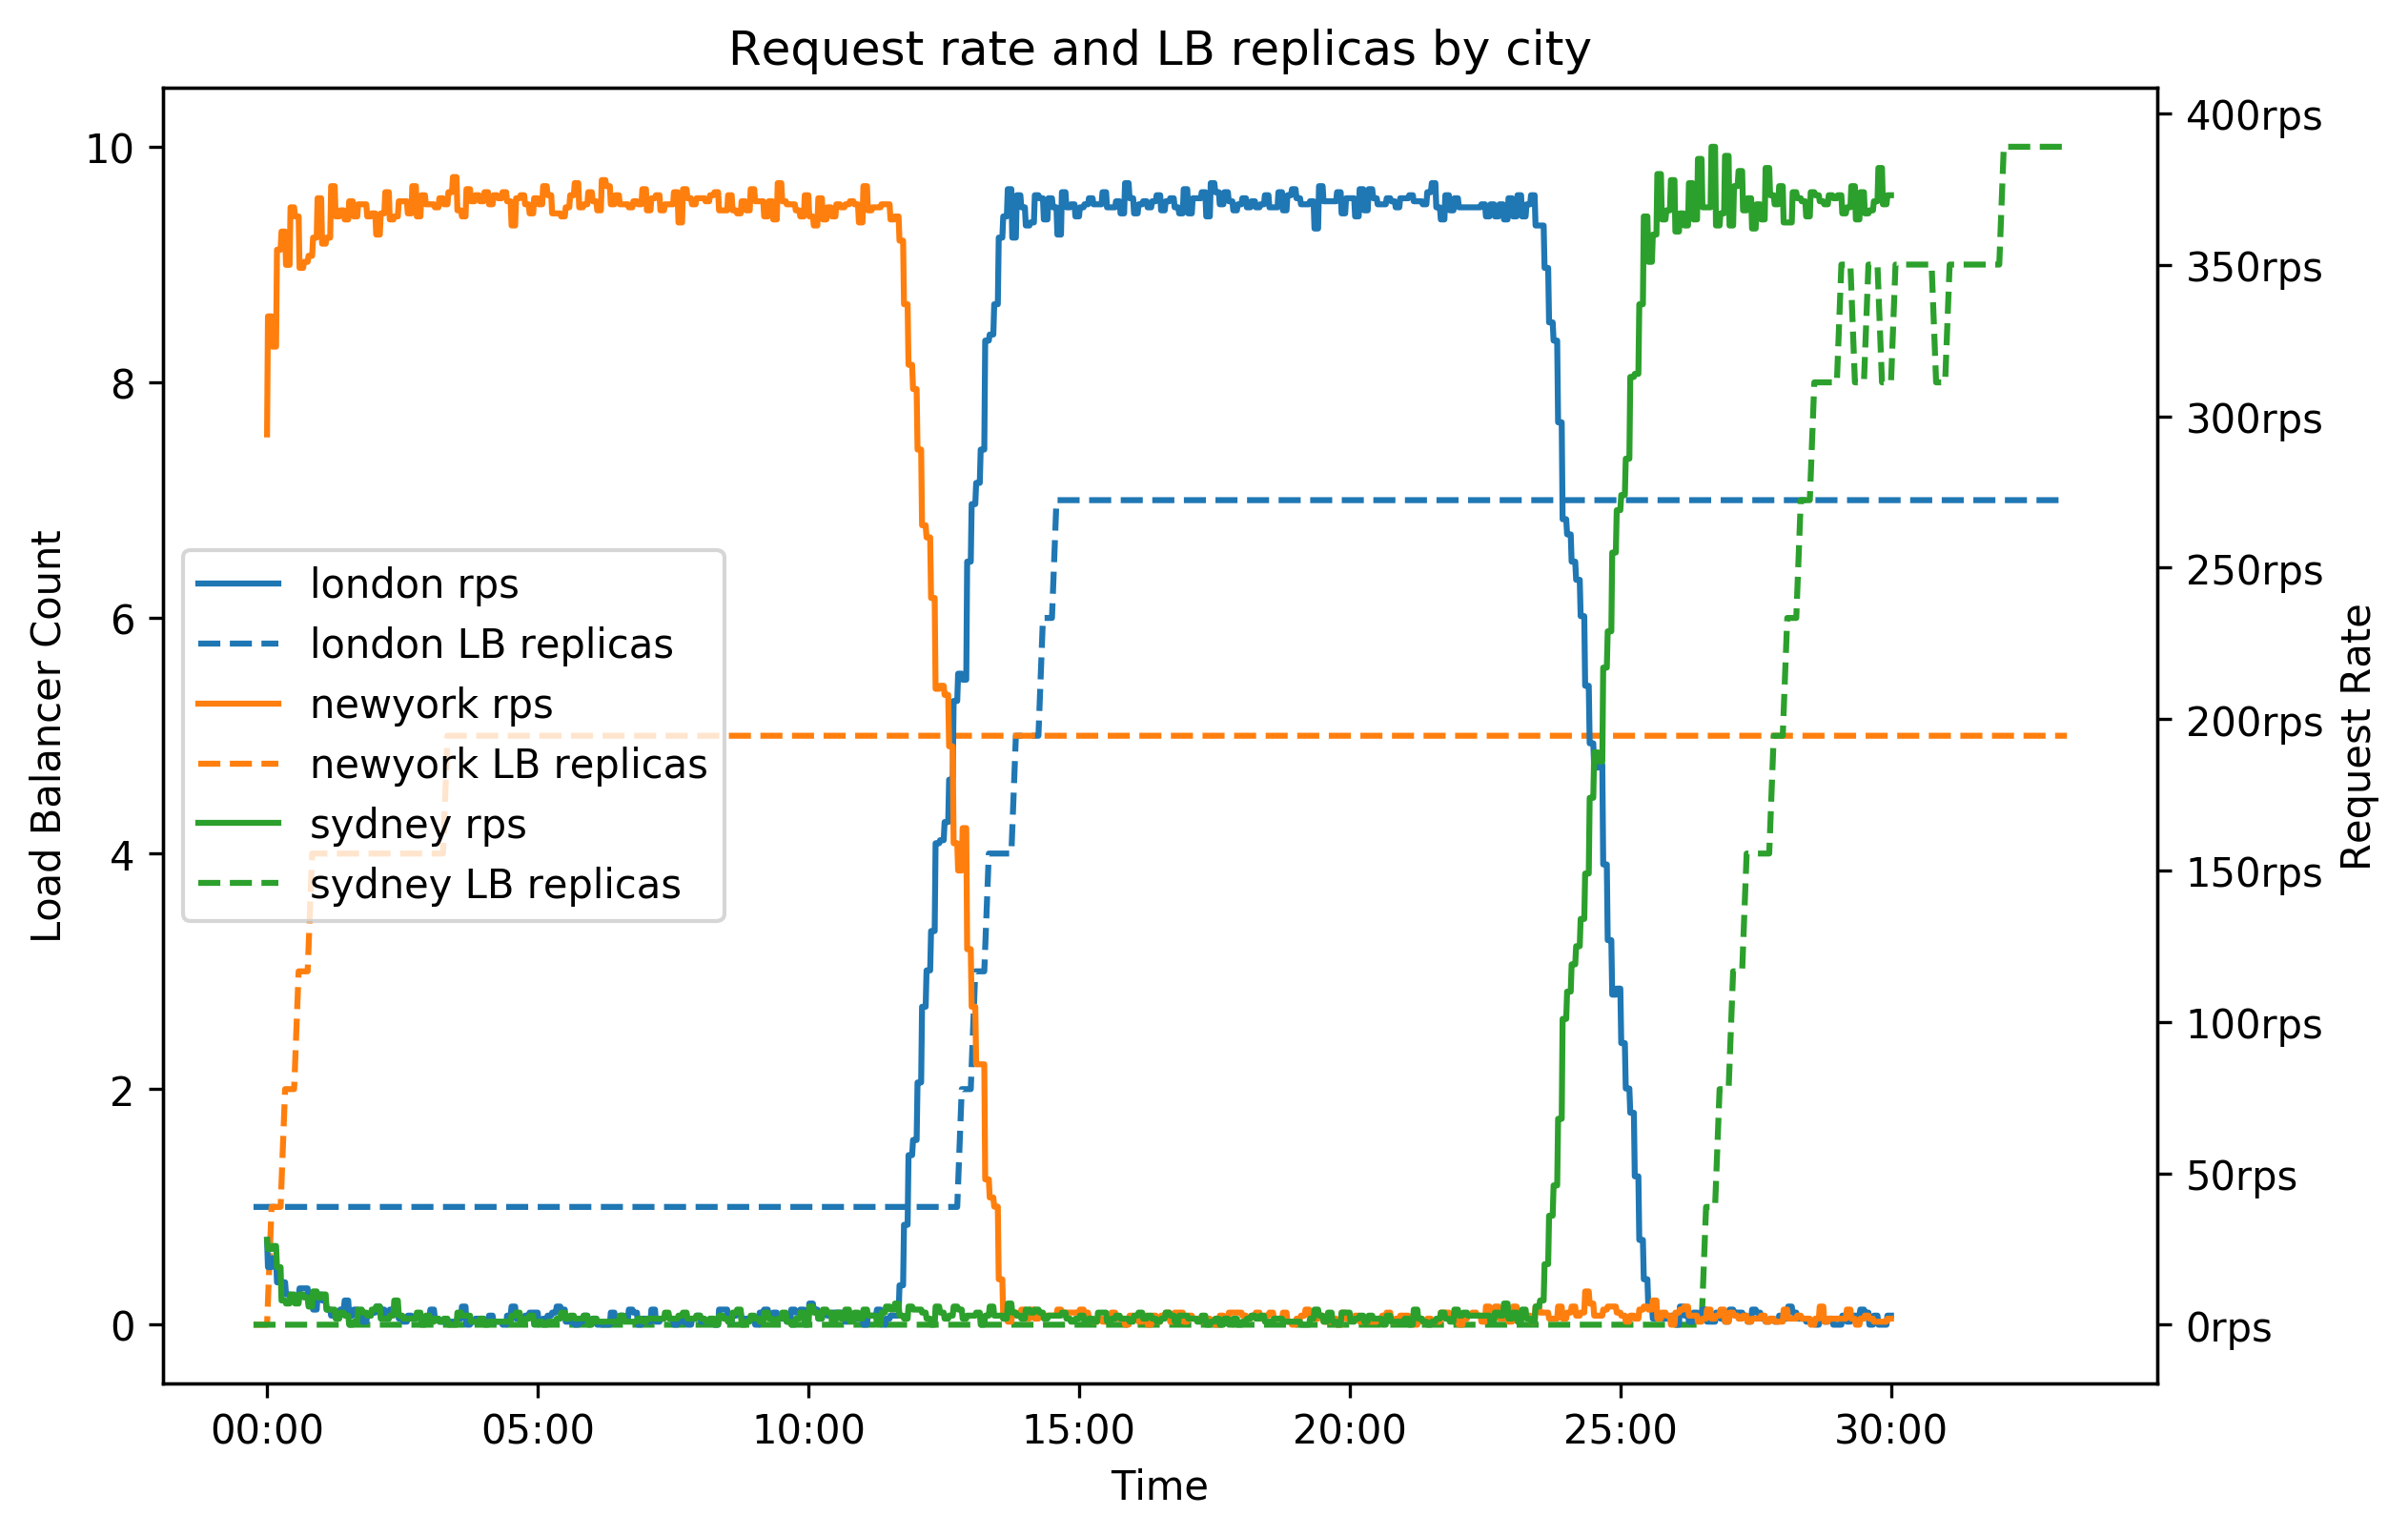
\includegraphics[width=14cm]{graphics/graphs/osmotic_dynamic_region_rps_lb_relicas_corrected.png}
    \caption{Load balancer replica count per city over changing request origins}
    \label{fig:osmotic_dynamic_lb_replicas}
\end{figure}

\begin{figure}
    \centering
    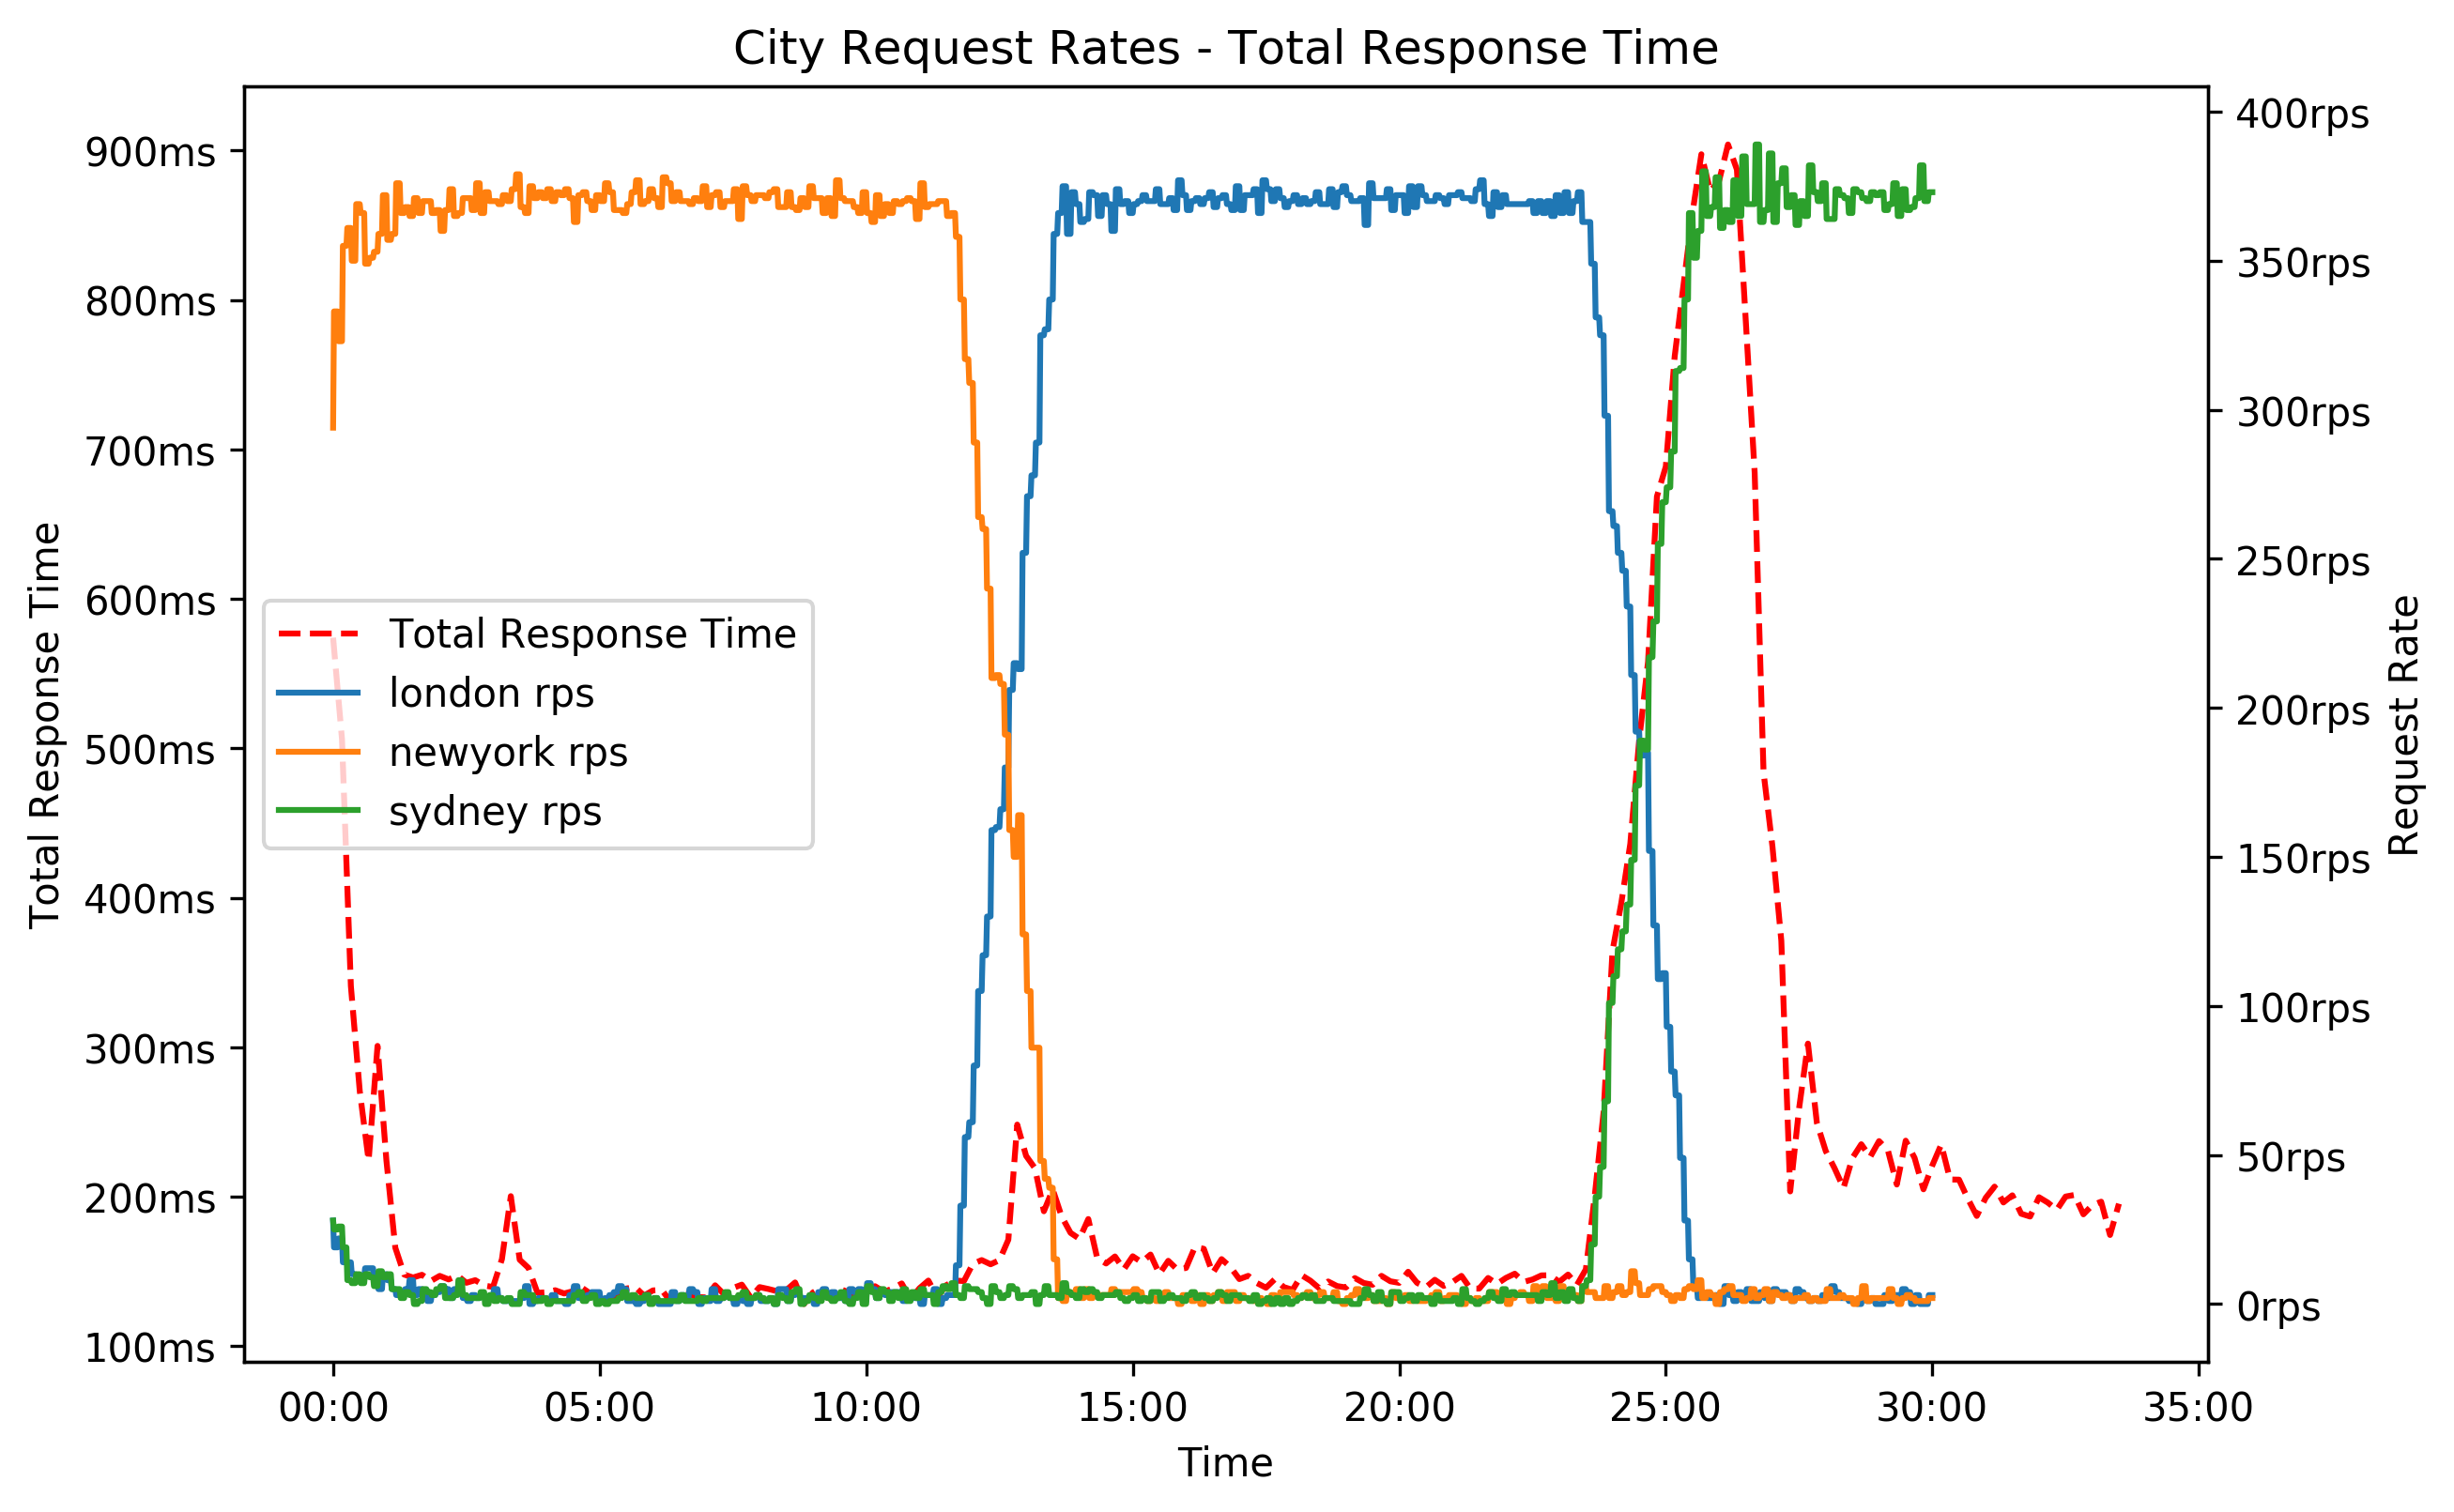
\includegraphics[width=14cm]{graphics/graphs/osmotic_dynamc_region_rps_trt_corrected.png}
    \caption{Total response time over changing request origins}
    \label{fig:osmotic_dynamic_trt}
\end{figure}

\begin{figure}
    \centering
    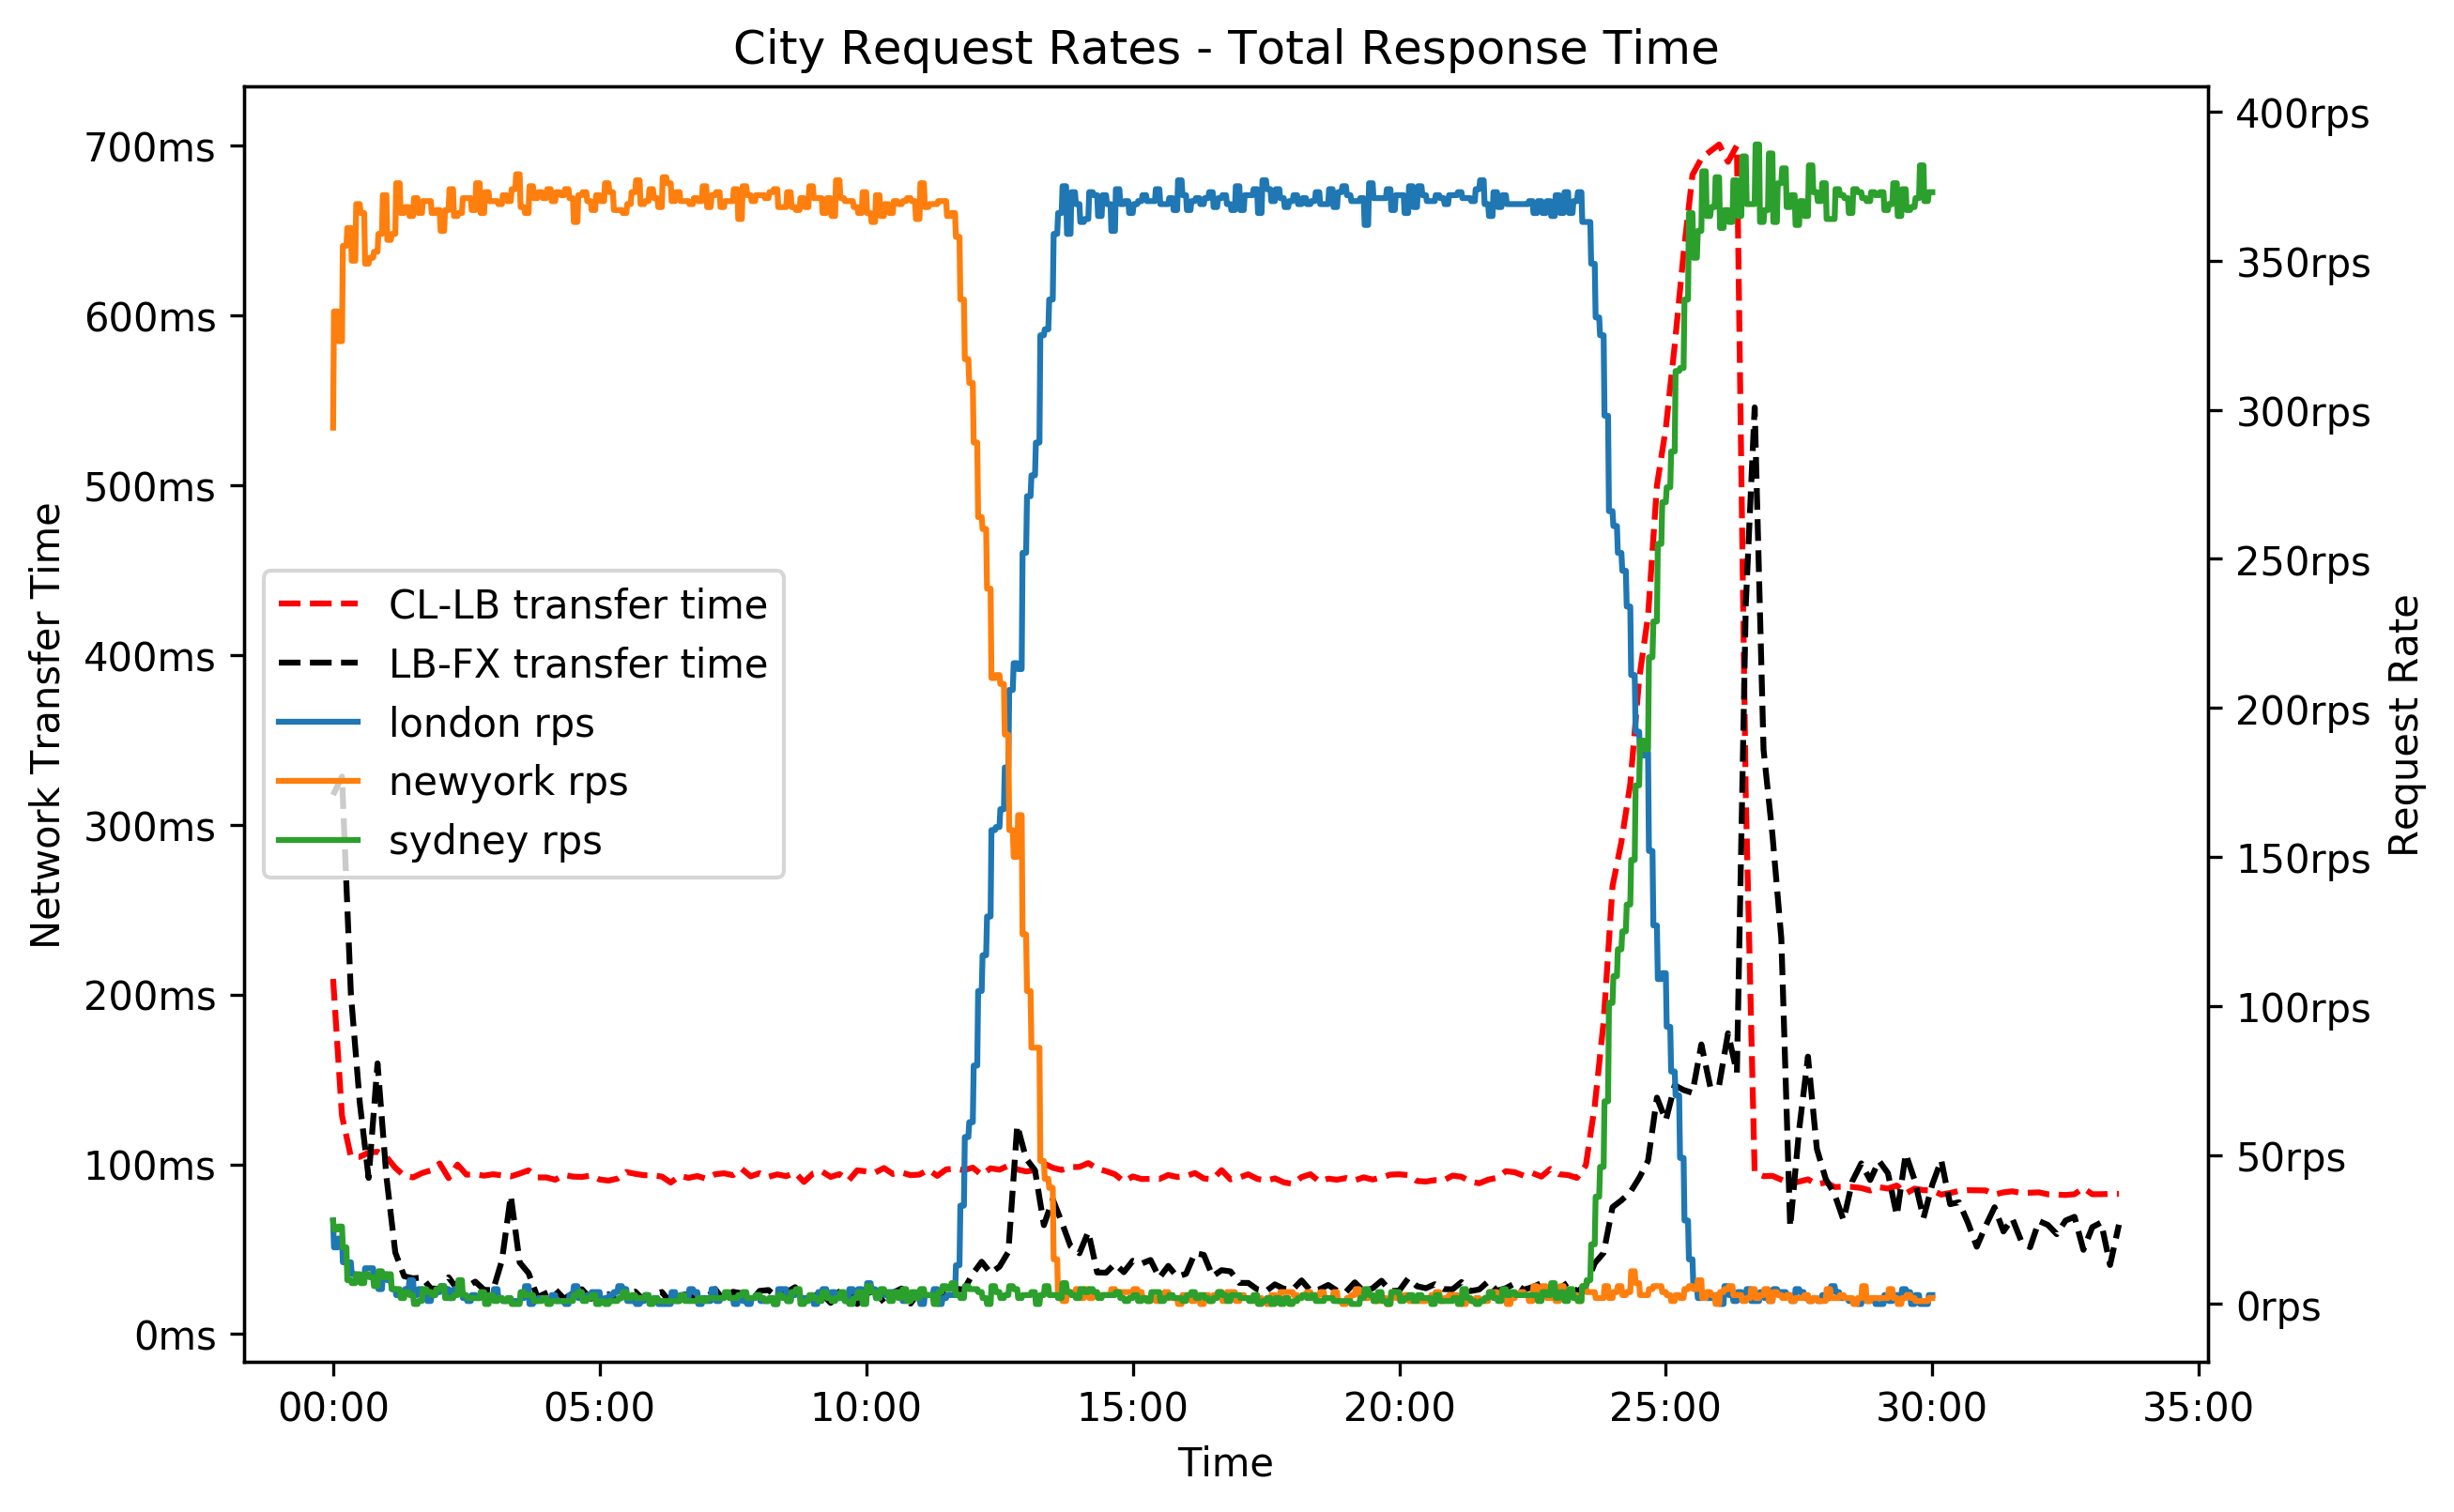
\includegraphics[width=14cm]{graphics/graphs/osmotic_dynamic_region_tx_times_corrected.png}
    \caption{Client to load balancer, and load balancer to function transfer times over changing request origins}
    \label{fig:osmotic_dynamic_tx}
\end{figure}

First of all, the results show that the osmotic scaling and scheduling component does indeed take the request origin into account when deciding on the number and location of new load balancer replicas.
Figure \ref{fig:osmotic_dynamic_lb_replicas} shows this in action.
While originally load balancers are only spawned in one city, because all requests originate from it, once requests start coming from another city, another load balancer instance is deployed in that city, as can be seen around timestamps 00:12 and 00:25 in Figure \ref{fig:osmotic_dynamic_lb_replicas}.

The effect this has on the system at large can also be observed easily, as Figure \ref{fig:osmotic_dynamic_trt} shows.
Here we can see that while the total response time of the system spikes once requests start to originate from another city, it starts to stabilize and come down to previous levels again once load balancers are present in the new city.
Please note that the \gls{trt} values shown in Figure \ref{fig:osmotic_dynamic_trt} are a moving average over a 10 second window, since this removes noise from the plot, making it more readable.
Likewise the request rate per city in Figures \ref{fig:osmotic_dynamic_lb_replicas}, \ref{fig:osmotic_dynamic_trt}, and \ref{fig:osmotic_dynamic_tx} is a moving average over a 5 second window, and displays the request rate for all functions deployed in the system.

Just like with the \gls{trt}, Figure \ref{fig:osmotic_dynamic_tx} shows that the request transfer time between client and load balancer, as well as between load balancer and function replica also spike when traffic originates from a different city.
There too, though we see that it returns to previous levels once load balancer replicas become available near the request origin.

% target: 9ish pages
\chapter{Discussion}
% target: 4ish pages

% Philipps DA: 1p intro, 1p per RQ, 1p future work
\chapter{Conclusion}
Edge computing has been proposed as a new computing paradigm to address the computational needs of new applications such as real-time cognitive assistance, large scale analytics from \gls{iot} sensors, or deep learning based image analysis on resource constrained devices.
Edge computing brings with it a number of significant implementation challenges.
In particular, edge computing environments are heterogeneous in hardware, software and networking conditions, featuring drastically different hardware, various operating systems, and a wide range of network conditions.
In addition to the system itself being heterogeneous, the surrounding conditions can be highly dynamic with request rates, clients, running applications, and the very structure of the system changing over time, in some scenarios even very quickly.

Currently, this complexity needs to be resolved by system developers themselves, which is not only very difficult, but is typically implementation-specific and thus not efficient in the long run.
Serverless computing has been proposed as an abstraction layer on top of edge computing systems with the goal of alleviating the need to deal with this complexity for developers.
Instead, the serverless edge computing framework is supposed to handle the tasks of scheduling and scaling functions, as well as routing them in such a way that the requirements of the application are fulfilled.
While serverless systems have been adapted to be edge-capable, there are some challenges that remain.
Network bound workloads in particular are an area where the performance of serverless edge computing systems was not in line with expectations.

This is the area of serverless edge computing this work aims to improve upon.
We perform an initial analysis of the load balancing component of the serverless system, which we suspect is the key component that needs to be adapted for network bound workloads to perform better.
Based on these results we propose to improve load balancing for serverless edge computing through two adaptations.
First, our approach changes the operating logic of the load balancer itself, moving away from the simple round robin load balancing current systems default to, towards a weighted response time implementation that tunes and adapts weights dynamically based on a least response time logic.
Second, we propose an osmotic pressure based approach to scaling and scheduling load balancer replicas, giving load balancers their own scaling and scheduling logic separate from the one regular serverless functions use, which allows the load balancer scheduling to consider the location of both function replicas and clients.

Results show that our approach not only significantly improves response times and network traffic of network bound workloads, but that it also opens up future opportunities for sophisticated deployment scenarios that have more differentiated performance requirements.

\section{Research Questions}
\section{Future Work}

% future work idea: it is relatively obvious that there is a non-linear relationship between load balancer scale and the performance limit they provide. The question now is how the linearity and scales here are influenced by the network itself. Can there, based on the network structure, be a way to determine the "optimal" number, or predict the impact sufficiently accurately that one can derive the "correct" scale given certain SLA requirements?

% how does information sharing between load balancerns contribute to their performance, and how can this be solved on an engineering-level to avoid exponential growth in data transfer sizes? also: how would the stochastic congestion game idea factor into this?

Our work provides a basis on which future work can be built, both to address limitations of our approach, as well as to further the capabilities of serverless edge computing.
This section provides a list of some of the most important areas for future work.
\begin{itemize}
    \item A continued evaluation of our approach in different deployment scenarios and network topologies could give further insight into its advantages and limitations. Based on this our approach could be changed to bring it closer to a state where it can reliably be used in real-world deployments.
    \item Building on our results, that show how response time percentiles and general service levels are influenced by load balancer scaling and implementation, a more sophisticated approach could be developed that takes into account and optimizes for different \gls{qos} levels on a per-function basis.
    \item In keeping with the previous point about different \gls{qos} levels, our approach could be modified to explicitly model the requirements of functions and then automatically tune its parameters accordingly. This would stand in contrast to current, statically configured implementations. In addition the need to do so is indicated by our experimental results, which show that for different environments different configurations are required to achieve optimal performance.
    \item Joint scheduling and scaling of functions and load balancers offers the potential for additional performance gains, where the information about required resources gathered by the load balancer could help make more informed decisions about function replica scale and location.
    \item Lastly, the topic of standardized edge computing scenarios for benchmarking remains a worthwhile area to improve upon. While there is effort to develop systematic benchmarks for edge computing, for example EdgeBench\cite{edgebench}, there is much to be done in terms of modelling network topologies and dynamically changing environments. Such a suite of standardized benchmarks and deployment scenarios would help to make competing approaches more directly comparable, and results more transparent.
    
\end{itemize}   
% \chapter{Introduction}
% \todo{Enter your text here.}

% \chapter{Additional Chapter}
% \todo{Enter your text here.}

% Remove following line for the final thesis.
% %% intro.tex
%% Copyright (C) 2014-2020 by Thomas Auzinger <thomas@auzinger.name>
%
% This work may be distributed and/or modified under the
% conditions of the LaTeX Project Public License, either version 1.3
% of this license or (at your option) any later version.
% The latest version of this license is in
%   http://www.latex-project.org/lppl.txt
% and version 1.3 or later is part of all distributions of LaTeX
% version 2005/12/01 or later.
%
% This work has the LPPL maintenance status `maintained'.
%
% The Current Maintainer of this work is Thomas Auzinger.
%
% This work consists of the files vutinfth.dtx and vutinfth.ins
% and the derived file vutinfth.cls.
% This work also consists of the file intro.tex.


\newacronym{ctan}{CTAN}{Comprehensive TeX Archive Network}
\newacronym{faq}{FAQ}{Frequently Asked Questions}
\newacronym{pdf}{PDF}{Portable Document Format}
\newacronym{svn}{SVN}{Subversion}
\newacronym{wysiwyg}{WYSIWYG}{What You See Is What You Get}

\newglossaryentry{texteditor}
{
  name={editor},
  description={A text editor is a type of program used for editing plain text files.}
}

\chapter{Introduction to \LaTeX}

Since \LaTeX\ is widely used in academia and industry, there exists a plethora of freely accessible introductions to the language.
Reading through the guide at \url{https://en.wikibooks.org/wiki/LaTeX} serves as a comprehensive overview for most of the functionality and is highly recommended before starting with a thesis in \LaTeX.

\section{Installation}

A full \LaTeX\ distribution\index{distribution} consists not only of the binaries that convert the source files to the typeset documents, but also of a wide range of packages and their documentation.
Depending on the operating system, different implementations are available as shown in Table~\ref{tab:distrib}.
\textbf{Due to the large amount of packages that are in everyday use and due to their high interdependence, it is paramount to keep the installed distribution\index{distribution} up to date.}
Otherwise, obscure errors and tedious debugging ensue.

\begin{table}
  \centering
  \begin{tabular}{cccc}
    \toprule
    Distribution & Unix         & Windows      & MacOS        \\
    \midrule
    TeX Live     & \textbf{yes} & yes          & (yes)        \\
    MacTeX       & no           & no           & \textbf{yes} \\
    MikTeX       & (yes)        & \textbf{yes} & yes          \\
    \bottomrule
  \end{tabular}
  \caption{\TeX/\LaTeX\ distributions for different operating systems. Recomended choice in \textbf{bold}.}
  \label{tab:distrib} % \label has to be placed AFTER \caption to produce correct cross-references.
\end{table}

\section{Editors}

A multitude of \TeX\ \glspl{texteditor} are available differing in their editing models, their supported operating systems and their feature sets.
A comprehensive overview of \glspl{texteditor} can be found at the Wikipedia page  \url{https://en.wikipedia.org/wiki/Comparison_of_TeX_editors}.
TeXstudio (\url{http://texstudio.sourceforge.net/}) is recommended.
Most editors support a synchronization of the generated document and the \LaTeX\ source by \verb|Ctrl| clicking either on the source document or the generated document.

\section{Compilation}

Modern editors usually provide the compilation programs to generate \gls{pdf} documents and for most \LaTeX\ source files, this is sufficient.
More advanced \LaTeX\ functionality, such as glossaries and bibliographies, needs additional compilation steps, however.
It is also possible that errors in the compilation process invalidate intermediate files and force subsequent compilation runs to fail.
It is advisable to delete intermediate files (\verb|.aux|, \verb|.bbl|, etc.), if errors occur and persist.
All files that are not generated by the user are automatically regenerated.
To compile the current document, the steps as shown in Table~\ref{tab:compile} have to be taken.


\begin{table}
  \centering
  \begin{tabular}{rl}
    \toprule
    & Description \\
    \midrule
    1 & Scan for refs, toc/lof/lot/loa items and cites \\
    2 & Build the bibliography     \\
    3 & Link refs and build the toc/lof/lot/loa \\
    4 & Link the bibliography \\
    5 & Build the glossary \\
    6 & Build the acronyms \\
    7 & Build the index \\
    8 & Link the glossary, acronyms, and the index \\
    9 & Link the bookmarks \\
    \midrule
    & Command \\
    \midrule
    1 & \verb|pdflatex.exe  example| \\
    2 & \verb|bibtex.exe    example| \\
    3 & \verb|pdflatex.exe  example| \\
    4 & \verb|pdflatex.exe  example| \\
    5 & \verb|makeindex.exe -t example.glg -s example.ist| \\
      & \verb|              -o example.gls example.glo| \\
    6 & \verb|makeindex.exe -t example.alg -s example.ist| \\
      & \verb|              -o example.acr example.acn| \\
    7 & \verb|makeindex.exe -t example.ilg -o example.ind example.idx| \\
    8 & \verb|pdflatex.exe  example| \\
    9 & \verb|pdflatex.exe  example| \\
    \bottomrule
  \end{tabular}
  \caption{Compilation steps for this document. The following abbreviations were used: table of contents (toc), list of figures (lof), list of tables (lot), list of algorithms (loa).}
  \label{tab:compile} % \label has to be placed AFTER \caption to produce correct cross-references.
\end{table}


\section{Basic Functionality}

In this section, various examples are given of the fundamental building blocks used in a thesis.
Many \LaTeX\ commands have a rich set of options that can be supplied as optional arguments.
The documentation of each command should be consulted to get an impression of the full spectrum of its functionality.

\subsection{Floats}

Two main categories of page elements can be differentiated in the usual \LaTeX\ workflow: \textit{(i)} the main stream of text and \textit{(ii)} floating containers that are positioned at convenient positions throughout the document.
In most cases, tables, plots, and images are put into such containers since they are usually positioned at the top or bottom of pages.
These are realized by the two environments \verb|figure| and \verb|table|, which also provide functionality for cross-referencing (see Table~\ref{tab:intro} and Figure~\ref{fig:intro}) and the generation of corresponding entries in the list of figures and the list of tables.
Note that these environments solely act as containers and can be assigned arbitrary content.

\subsection{Tables}

A table in \LaTeX\ is created by using a \verb|tabular| environment or any of its extensions, e.g., \verb|tabularx|.
The commands \verb|\multirow| and \verb|\multicolumn| allow table elements to span multiple rows and columns.

\begin{table}[h] % placement specifier
  \centering
  \begin{tabular}{lll}
    \toprule
    \multicolumn{2}{c}{Position} \\
    \cmidrule{1-2} % partial horizontal rule
    Group & Abbrev & Name \\
    \midrule
    Goalkeeper & GK & Paul Robinson \\
    \midrule
    \multirow{4}{*}{Defenders} & LB & Lucus Radebe \\
                               & DC & Michael Duburry \\
                               & DC & Dominic Matteo \\
                               & RB & Didier Domi \\
    \midrule
    \multirow{3}{*}{Midfielders} & MC & David Batty \\
                                 & MC & Eirik Bakke \\
                                 & MC & Jody Morris \\
    \midrule
    Forward & FW & Jamie McMaster \\
    \midrule
    \multirow{2}{*}{Strikers} & ST & Alan Smith \\
                              & ST & Mark Viduka \\
    \bottomrule
  \end{tabular}
  \caption{Adapted example from the \LaTeX guide at \url{https://en.wikibooks.org/wiki/LaTeX/Tables}. This example uses rules specific to the \texttt{booktabs} package and employs the multi-row functionality of the \texttt{multirow} package.}
  \label{tab:intro} % \label has to be placed AFTER \caption to produce correct cross-references.
\end{table}

\subsection{Images}

An image is added to a document via the \verb|\includegraphics| command as shown in Figure~\ref{fig:intro}.
The \verb|\subcaption| command can be used to reference subfigures, such as Figure~\ref{fig:intro:full width} and~\ref{fig:intro:half width}.

\begin{figure}[h]
  \centering
  \begin{subfigure}[b]{0.45\columnwidth}
    \centering
    
\includegraphics[width=\textwidth]{Logo-schwarz.pdf}
    \subcaption{The header logo at text width.}
    \label{fig:intro:full width}
  \end{subfigure}
  \begin{subfigure}[b]{0.45\columnwidth}
    \centering
    
\includegraphics[width=0.5\textwidth]{Logo-schwarz.pdf}
    \subcaption{The header logo at half the text width.}
    \label{fig:intro:half width}
  \end{subfigure}
  \caption[Optional caption for the figure list (often used to abbreviate long captions)]{The header logo at different sizes.} % Remove the [...] argument if the original caption should be used in the figure list.
  \label{fig:intro} % \label has to be placed AFTER \caption (or \subcaption) to produce correct cross-references.
\end{figure}

\subsection{Mathematical Expressions}

One of the original motivation to create the \TeX\ system was the need for mathematical typesetting.
To this day, \LaTeX\ is the preferred system to write math-heavy documents and a wide variety of functions aids the author in this task.
A mathematical expression can be inserted inline as $\sum_{n=1}^{\infty} \frac{1}{n^2} = \frac{\pi^2}{6}$ outside of the text stream as \[ \sum_{n=1}^{\infty} \frac{1}{n^2} = \frac{\pi^2}{6} \] or as numbered equation with
\begin{equation}
\sum_{n=1}^{\infty} \frac{1}{n^2} = \frac{\pi^2}{6}.
\end{equation}

\subsection{Pseudo Code}

The presentation of algorithms can be achieved with various packages; the most popular are \verb|algorithmic|, \verb|algorithm2e|, \verb|algorithmicx|, or \verb|algpseudocode|.
An overview is given at \url{https://tex.stackexchange.com/questions/229355}.
An example of the use of the \verb|alogrithm2e| package is given with Algorithm~\ref{alg:gauss-seidel}.

\begin{algorithm}
  \SetKw{BreakFor}{break for}
  \KwIn{A scalar~$\epsilon$, a matrix $\mathbf{A} = (a_{ij})$, a vector $\vec{b}$, and an initial vector $\vec{x}^{(0)}$}
  \KwOut{$\vec{x}^{(n)}$ with $\mathbf{A} \vec{x}^{(n)} \approx \vec{b}$}
  \For{$k\leftarrow 1$ \KwTo maximum iterations}
  {
     \For{$i\leftarrow 1$ \KwTo $n$}
     {
        $x_i^{(k)} = \frac{1}{a_{ii}} \left(b_i-\sum_{j<i} a_{ij} x_j^{(k)} - \sum_{j>i} a_{ij} x_j^{(k-1)} \right)$\;
     }
     \If{$\lvert\vec{x}^{(k)}-\vec{x}^{(k-1)}\rvert < \epsilon$}
     {\BreakFor\;}
  }
  \Return{$\vec{x}^{(k)}$\;}
  \caption{Gauss-Seidel}
  \label{alg:gauss-seidel} % \label has to be placed AFTER \caption to produce correct cross-references.
\end{algorithm}

\section{Bibliography}

The referencing of prior work is a fundamental requirement of academic writing and well supported by \LaTeX.
The \textsc{Bib}\TeX\ reference management software is the most commonly used system for this purpose.
Using the \verb|\cite| command, it is possible to reference entries in a \verb|.bib| file out of the text stream, e.g., as~\cite{Turing1936}.
The generation of the formatted bibliography needs a separate execution of \verb|bibtex.exe| (see Table~\ref{tab:compile}).

\section{Table of Contents}

The table of contents is automatically built by successive runs of the compilation, e.g., of \verb|pdflatex.exe|.
The command \verb|\setsecnumdepth| allows the specification of the depth of the table of contents and additional entries can be added to the table of contents using \verb|\addcontentsline|.
The starred versions of the sectioning commands, i.e., \verb|\chapter*|, \verb|\section*|, etc., remove the corresponding entry from the table of contents.

\section{Acronyms / Glossary / Index}

The list of acronyms, the glossary, and the index need to be built with a separate execution of \verb|makeindex| (see Table~\ref{tab:compile}).
Acronyms have to be specified with \verb|\newacronym| while glossary entries use \verb|\newglossaryentry|.
Both are then used in the document content with one of the variants of \verb|\gls|, such as \verb|\Gls|, \verb|\glspl|, or \verb|\Glspl|.
Index items are simply generated by placing \verb|\index|\marg{entry} next to all the words that correspond to the index entry \meta{entry}.
Note that many enhancements exist for these functionalities and the documentation of the \verb|makeindex| and the \verb|glossaries| packages should be consulted.

\section{Tips}

Since \TeX\ and its successors do not employ a \gls{wysiwyg} editing scheme, several guidelines improve the readability of the source content:
\begin{itemize}
\item Each sentence in the source text should start with a new line.
      This helps not only the user navigation through the text, but also enables revision control systems (e.g. \gls{svn}, Git) to show the exact changes authored by different users.
      Paragraphs are separated by one (or more) empty lines.
\item Environments, which are defined by a matching pair of \verb|\begin{name}| and \verb|\end{name}|, can be indented by whitespace to show their hierarchical structure.
\item In most cases, the explicit use of whitespace (e.g. by adding \verb|\hspace{4em}| or \verb|\vspace{1.5cm}|) violates typographic guidelines and rules.
      Explicit formatting should only be employed as a last resort and, most likely, better ways to achieve the desired layout can be found by a quick web search.
\item The use of bold or italic text is generally not supported by typographic considerations and the semantically meaningful \verb|\emph{|\texttt{$\dots$}\verb|}| should be used.
\end{itemize}

The predominant application of the \LaTeX\ system is the generation of \gls{pdf} files via the \textsc{Pdf}\LaTeX\ binaries.
In the current version of \textsc{Pdf}\LaTeX, it is possible that absolute file paths and user account names are embedded in the final \gls{pdf} document.
While this poses only a minor security issue for all documents, it is highly problematic for double blind reviews.
The process shown in Table~\ref{tab:ps2pdf} can be employed to strip all private information from the final \gls{pdf} document.

\begin{table}[h]
  \centering
  \begin{tabular}{rl}
  \toprule
  & Command \\
  \midrule
  1 & Rename the \gls{pdf} document \verb|final.pdf| to \verb|final.ps|. \\
  2 & Execute the following command: \\
    & \verb|ps2pdf -dPDFSETTINGS#/prepress ^| \\
    & \verb| -dCompatibilityLevel#1.4 ^| \\
    & \verb| -dAutoFilterColorImages#false ^| \\
    & \verb| -dAutoFilterGrayImages#false ^| \\
    & \verb| -dColorImageFilter#/FlateEncode ^| \\
    & \verb| -dGrayImageFilter#/FlateEncode ^| \\
    & \verb| -dMonoImageFilter#/FlateEncode ^| \\
    & \verb| -dDownsampleColorImages#false ^| \\
    & \verb| -dDownsampleGrayImages#false ^| \\
    & \verb| final.ps final.pdf| \\
  \bottomrule
  \end{tabular}

  On Unix-based systems, replace \verb|#| with \verb|=| and \verb|^| with \verb|\|.
  \caption{Anonymization of \gls{pdf} documents.}
  \label{tab:ps2pdf}
\end{table}

\section{Resources}

\subsection{Useful Links}

In the following, a listing of useful web resources is given.
\begin{description}
\item[\url{https://en.wikibooks.org/wiki/LaTeX}] An extensive wiki-based guide to \LaTeX.
\item[\url{http://www.tex.ac.uk/faq}] A (huge) set of \gls{faq} about \TeX\ and \LaTeX.
\item[\url{https://tex.stackexchange.com/}] The definitive user forum for non-trivial \LaTeX-related questions and answers.
\end{description}

\subsection[Comprehensive TeX Archive Network]{\gls{ctan}}

The \gls{ctan} is the official repository for all \TeX\ related material.
It can be accessed via \url{https://www.ctan.org/} and hosts (among other things) a huge variety of packages that provide extended functionality for \TeX\ and its successors.
Note that most packages contain \gls{pdf} documentation that can be directly accessed via \gls{ctan}.

In the following, a short, non-exhaustive list of relevant \gls{ctan}-hosted packages is given together with their relative path.
\begin{description}[itemsep=0ex]
\item[\href{https://www.ctan.org/pkg/algorithm2e}{algorithm2e}] Functionality for writing pseudo code.
\item[\href{https://www.ctan.org/pkg/amsmath}{amsmath}] Enhanced functionality for typesetting mathematical expressions.
\item[\href{https://www.ctan.org/pkg/amsfonts}{amssymb}] Provides a multitude of mathematical symbols.
\item[\href{https://www.ctan.org/pkg/booktabs}{booktabs}] Improved typesetting of tables.
\item[\href{https://www.ctan.org/pkg/enumitem}{enumitem}] Control over the layout of lists (\verb|itemize|, \verb|enumerate|, \verb|description|).
\item[\href{https://www.ctan.org/pkg/fontenc}{fontenc}] Determines font encoding of the output.
\item[\href{https://www.ctan.org/pkg/glossaries}{glossaries}] Create glossaries and list of acronyms.
\item[\href{https://www.ctan.org/pkg/graphicx}{graphicx}] Insert images into the document.
\item[\href{https://www.ctan.org/pkg/inputenc}{inputenc}] Determines encoding of the input.
\item[\href{https://www.ctan.org/pkg/l2tabu}{l2tabu}] A description of bad practices when using \LaTeX.
\item[\href{https://www.ctan.org/pkg/mathtools}{mathtools}] Further extension of mathematical typesetting.
\item[\href{https://www.ctan.org/pkg/memoir}{memoir}] The document class on upon which the \verb|vutinfth| document class is based.
\item[\href{https://www.ctan.org/pkg/multirow}{multirow}] Allows table elements to span several rows.
\item[\href{https://www.ctan.org/pkg/pgfplots}{pgfplots}] Function plot drawings.
\item[\href{https://www.ctan.org/pkg/pgf}{pgf/TikZ}] Creating graphics inside \LaTeX\ documents.
\item[\href{https://www.ctan.org/pkg/subcaption}{subcaption}] Allows the use of subfigures and enables their referencing.
\item[\href{https://www.ctan.org/tex-archive/info/symbols/comprehensive/}{symbols/comprehensive}] A listing of around 5000 symbols that can be used with \LaTeX.
\item[\href{https://www.ctan.org/pkg/voss-mathmode}{voss-mathmode}] A comprehensive overview of typesetting mathematics in \LaTeX.
\item[\href{https://www.ctan.org/pkg/xcolor}{xcolor}] Allows the definition and use of colors.
\end{description} % A short introduction to LaTeX.

\backmatter

% Use an optional list of figures.
\listoffigures % Starred version, i.e., \listoffigures*, removes the toc entry.

% Use an optional list of tables.
\cleardoublepage % Start list of tables on the next empty right hand page.
\listoftables % Starred version, i.e., \listoftables*, removes the toc entry.

% Use an optional list of alogrithms.
\listofalgorithms
\addcontentsline{toc}{chapter}{List of Algorithms}

% Add an index.
\printindex

% Add a glossary.
\printglossaries

% Add a bibliography.
\bibliographystyle{alphaurl}
\bibliography{main}

\end{document}